\documentclass[12pt, a4paper, liststotoc]{scrreprt}

\usepackage{ngerman}
\usepackage[utf8]{inputenc}

\usepackage{tipa}
\usepackage{here} 

%\usepackage[T1]{fontenc}

\usepackage{comment}

\usepackage{listings} 

\usepackage{blindtext}
\usepackage{fancyhdr} %Fuer Kopf und Fusszeilen
\usepackage{anysize} %Damit man Raender leicht einstellen kann
\usepackage{titlesec}

\usepackage{bookmark,hyperref}

\usepackage{tabularx}
\usepackage{rotating}
\usepackage{hhline}

%\usepackage{float}
\usepackage{floatrow}
%\usepackage[sc,center]{titlesec} %Um Kapitelnamen-Schrift zu veraendern
%\usepackage[T1]{fontenc} %ueblich
\usepackage{subfigure}

%\renewcommand{\thesubfigure}{\thefigure.\arabic{subfigure}}
%\makeatletter
%\renewcommand{\p@subfigure}{}
%\renewcommand{\@thesubfigure}{\thesubfigure:\hskip\subfiglabelskip}
%\makeatother

%\makeindex

%Paket zum importieren von Bildern
\usepackage{graphicx}
\newcommand{\HRule}{\rule{\linewidth}{0.2mm}}
\usepackage{tikz}
\usetikzlibrary{trees}

\usepackage{pageslts}
\usepackage{thumbs}
\usepackage{hyperref}

\usepackage{tabularx}

\usepackage{wrapfig} % Paket zur Positionierung einbinden

\usepackage{bibgerm}

\usepackage{amssymb} % Mathe Symbole
\usepackage{amsmath} % Mathe

\usepackage{booktabs}
\usepackage{subfigure}

\usepackage[nottoc]{tocbibind}

%Zeilenabstand ist jetzt 1.5 fach
\usepackage{setspace}
\onehalfspacing 
%Bilder werden auch im Unterverzeichnis img gesucht
\graphicspath{{img/}} 

\usepackage[Algorithmus]{algorithm}
\usepackage{algorithmic}

%Raender
%\marginsize{3.5cm}{1.5cm}{2.5cm}{2.5cm}
%\marginsize{3.5cm}{1.75cm}{2.5cm}{2.25cm}

\definecolor{haw_rot}{RGB}{160,0,0}
\definecolor{lgrey}{RGB}{240,240,240}


\newcommand{\mytoprule}{\specialrule{0.12em}{0em}{0em}}
\newcommand{\mybottomrule}{\specialrule{0.12em}{0em}{0em}} 
\renewcommand{\arraystretch}{1.2}

\usepackage{placeins}

%\renewcommand{\thesubfigure}{\thefigure.\arabic{subfigure}}
%\makeatletter
%\renewcommand{\p@subfigure}{}
%\renewcommand{\@thesubfigure}{\thesubfigure:\hskip\subfiglabelskip}
%\makeatother

%\makeindex
\usepackage{courier}
\lstset{ basicstyle=\small\ttfamily,
		 breaklines=true,}

\hyphenation{
}
\begin{document}


%pagenumbering wird benoetigt um Warnung zu beheben.
%wird wieder ueberschrieben
\pagenumbering{Roman}
\begin{titlepage}


\begin{center}


% Upper part of the page
%\begin{flushleft}
%
\includegraphics[angle=0,width=10cm]{./img/HL_WBM_de_B_300dpi.jpg}\\[3cm]    
%\end{flushleft}

%\textsc{\LARGE Hochschule Landshut}\\[1.5cm]

\includegraphics[angle=0,width=7cm]{./img/HL_WBM_de_B_300dpi.jpg}\\[2cm]


\textsc{\LARGE Masterarbeit}\\[0.6cm]

\small 

am Labor für medizinische Bildverarbeitung, Algorithmen und Krankenhaus IT \\[1cm]
zur Erlangung des akademischen Grades\\
\textbf{Master of Science (M. Sc.)} \\[1cm]

\normalsize

% Title
\HRule \\[0.4cm]
{
	
	\bfseries Entwicklung einer modularen und erweiterbaren Anwendung \\
	 zur medizinischen Bildverarbeitung
}\\[0.4cm]
\HRule \\[1.3cm]






%{\large \today}

\vfill

\footnotesize 

\begin{tabularx}{\textwidth}{Xr}
  \textbf{eingereicht von} 	& 	Rudolf Franz Siegfried Korb, 790060 \\ 
  \textbf{Erstprüfer} 		& 	Prof., Dr. Holger Timinger \\ 
  \textbf{Zweitprüferin} 	& 	Prof., Dr. Gudrun Schiedermeier \\ 
  \textbf{Abgabetermin}		&	02.03.2014
\end{tabularx}

\end{center}

%Bottom of page
% Author and supervisor
%\begin{minipage}{0.4\textwidth}
%\begin{flushleft} 
%\emph{Autor:}\\
%Rudolf Korb
%\end{flushleft}
%\end{minipage}
%\hfill
%\begin{minipage}{0.4\textwidth}
%\begin{flushright} 
%\emph{Betreuer:} \\
%Prof., Dr. Holger Timinger \\
%Prof., Dr. Gudrun Schiedermeier
%\end{flushright}
%\end{minipage}





\end{titlepage}

\pagestyle{empty}
% Das folgende braucht man, damit auch wirklich 1 Leerseite gelassen wird
\mbox{}
\clearpage

%Veraendert die Seitennummerierung zu roemischen Zeichen...
\setcounter{page}{1}

\renewcommand{\thepage}{\roman{page}}
%\pagestyle{headings}

\tableofcontents


\pagebreak

\renewcommand{\thepage}{\arabic{page}}
\setcounter{page}{1}

%Thumbverzeichnis
\addthumbsoverviewtocontents{chapter}{Kapitelübersicht}%Schreibt die Kapitelübersicht als Kapitel ins TOC
\thumbsoverview{Kapitelübersicht} 

\pagestyle{fancy} %eigener Seitenstil
\fancyhf{} %alle Kopf- und Fußzeilenfelder bereinigen
\renewcommand{\chaptermark}[1]{ \markboth{#1}{} }
\fancyhead[L]{\leftmark} %Kopfzeile links
%\fancyhead[C]{} %zentrierte Kopfzeile
%\fancyhead[R]{} %Kopfzeile rechts

%\fancyhead[R]{\textit{ \nouppercase{\leftmark}} }
%\fancyhead[L]{\textit{ \nouppercase{\rightmark}} }

\renewcommand{\headrulewidth}{0.3pt} %obere Trennlinie
\fancyfoot[C]{\thepage} %Seitennummer
\renewcommand{\footrulewidth}{0.3pt} %untere Trennlinie

\chapter{Einleitung}\label{einleitung}
\addthumb{Einleitung}{\huge{\textbf{\thechapter.}}}{white}{haw_rot} 

Ziel dieser Abschlussarbeit ist die Entwicklung einer Software zur medizinischen Bildverarbeitung. Eine modulare und flexible Architektur soll eine leichte Erweiterbarkeit sowohl für Entwickler (Erstellen eigener Werkzeuge) als auch den Anwender (Integration selbst implementierter Bildverarbeitungsalgorithmen) ermöglichen.\\
Das Programm soll für Forschung und Lehre am Labor für medizinische Bildverarbeitung, Algorithmen und Krankenhaus IT eingesetzt werden. Nach einer Vorstellung des Labors und dem zugehörigen Studiengang der biomedizinischen Technik erfolgt die Analyse der Anforderungen der Software. Aufbauend werden einige Grundlagen zur medizinischen Bildverarbeitung dargestellt. Der Fokus liegt auf dem DICOM-Standard und den Eigenschaften der medizinischen Bilddaten. Das nächste Kapitel erläutert die Softwarearchitektur sowie die Implementierung. Praktische Anwendungsbeispiele schließen die technischen Aspekte der Arbeit ab. Die folgende Diskussion zeigt Erweiterungsmöglichkeiten für die zukünftige Entwicklung auf.

\section{Der sechste Kondratieff-Zyklus}
Im Jahr 1926 veröffentlichte der Wirtschaftswissenschaftler Nikolai D. Kondratieff (* 1892, \dag 1938) die Theorie \glqq Die Langen Wellen der Konjunktur\grqq\ \cite{hensen:gesundeGesellschaft}.
Leo Nefiodow erweiterte 2006 die Theorie, damit die Entwicklung des 20. Jahrhunderts einfließen konnte.\\
Kondratieff zeigte, dass sich die gesellschaftliche Wandlung nicht willkürlich vollzog. Seit der Industrialisierung Mitte des 18. Jahrhunderts stand der Wohlstand der Gesellschaft in direkter Beziehung zu besonderen Erfindungen. Er betrachtete die Phasen des Wohlstandes und die direkt folgende Wirtschaftskrise und entdeckte die später nach ihm benannten \glqq Kondratieff-Zyklen\grqq\.
Wie in Abbildung \ref{zyklen} zu sehen ist, war die Dampfmaschine die erste Basisinnovation\footnote{Basisinnovationen müssen nach Nefiodow vier Eigenschaften erfüllen: Entstehung eines neuen Marktes mit vielen Arbeitsplätzen; Innovation bestimmt den Zyklus; Basisinnovationen haben einen Zyklus von 40 - 60 Jahren; Sie bestimmen die Entwicklungsrichtung} und revolutionierte die Textilindustrie.\cite{wieden:liquidwork}

%\begin{wrapfigure}{c}{10cm}
%\centering
%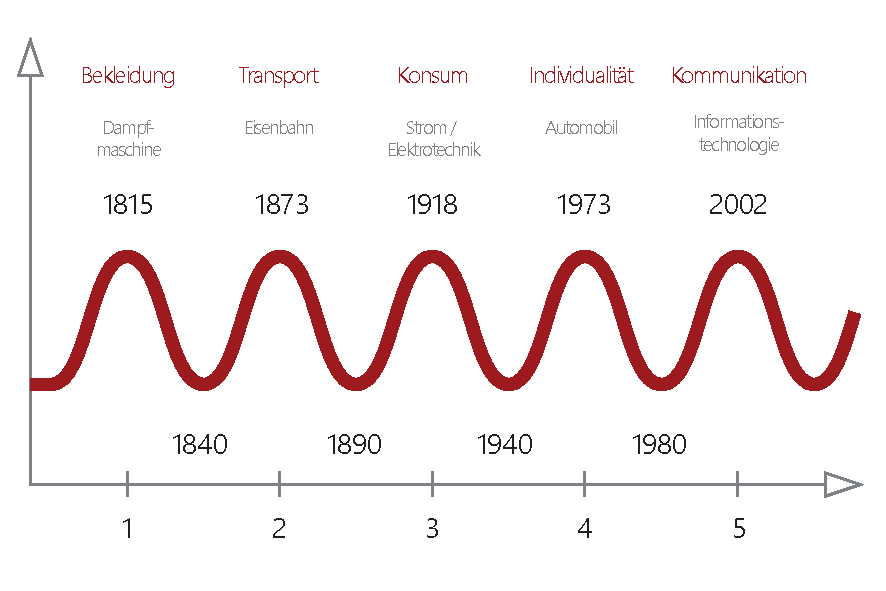
\includegraphics[width=8cm]{./img/zyklen.pdf}
%\caption{Kontratieff Zyklen}
%\label{zyklen}
%\end{wrapfigure}

\begin{figure}[htbp]
  \vspace{0.5cm}
  \centering
  \fbox{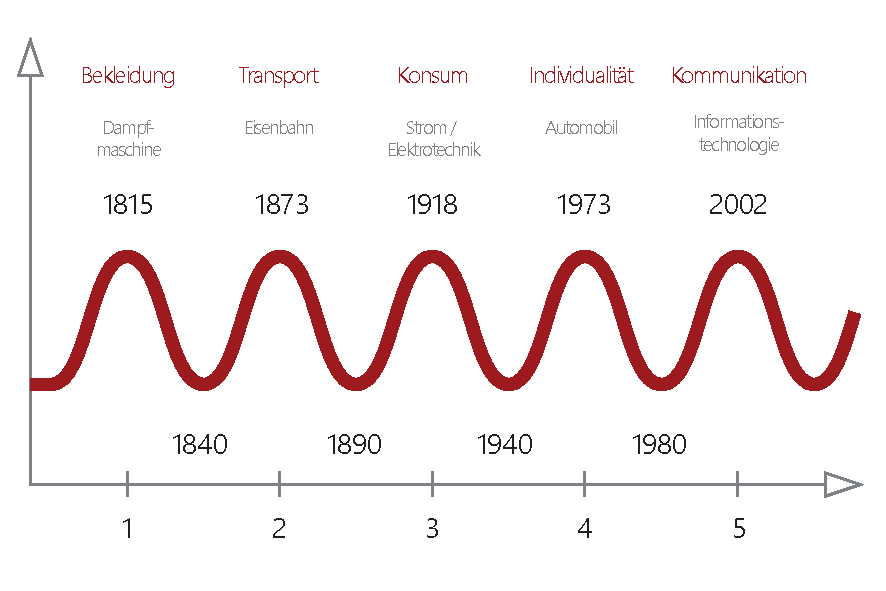
\includegraphics[angle=0,width=12cm]{./img/zyklen.pdf}}
  \caption{Kondratieff-Zyklen}
  \label{zyklen}
  \vspace{0.5cm}
\end{figure}

Diese Erfindung gilt als Beginn des ersten Kondratieff-Zyklus. Vor dem maschinellen Betrieb wurden Spinnräder noch manuell bedient und Kleidung war teuer. Die dampfbetriebenen Webstühle steigerten
die Effizienz um das 200-fache. In den 20er Jahren stagnierte die Branche, da die Rohstoffbeschaffung und Warenverteilung das Maximum der Effizienz erreicht hatte. Mit der Erfindung der Eisenbahn gelang der Übergang vom ersten in den zweiten Zyklus. In den folgenden Jahren konnte nun das Bedürfnis nach verbesserten Transportmöglichkeiten gestillt werden.\\
Dampfmaschine, Eisenbahn, Strom, Motor und der Mikrochip stehen alle für eine Basisinnovation, die zukünftige Gesellschaften geprägt haben. Im lauf der Zeit verschwinden die Erfindungen aus dem Bewusstsein der Menschen und werden zu Gegenständen des Alltags. Motor und Mikrochip sind so stark im gesellschaftlichen Leben verankert, dass sie nicht mehr direkt wahrgenommen werden. Betrachtet man eine elektrische Zahnbürste, ist es selbstverständlich, dass die Energie aus dem Stromnetz bezogen wird und der Bürstenkopf von einem Motor angetrieben wird.\\
Das Jahr 2002 gilt als Höhepunkt des fünften Kondratieff-Zyklus und die Gesellschaft befindet sich gerade im Übergang zum Sechsten. Noch fehlt die aktuelle Basisinnovation und auch das zu stillende Bedürfnis ist nach der Kommunikation noch nicht bestimmt.\\
Nach Nefiodow \cite{nefiodow:gesundheit} gibt es vier Möglichkeiten welcher Markt in Zukunft den sechsten Kondratieff prägen wird:
\begin{itemize}
  \item \textbf{Informationsmarkt} \\
  		Mobile Geräte und Soziale Netzwerke sind maßgebend für diesen Markt. So verhalf der Kurznachrichtendienst Twitter zum sogenannten \glqq Arabischen Frühling\grqq\, durch die blitzschnelle Kommunikation über das Netz\footnote{http://www.heise.de/tr/blog/artikel/Wie-funktioniert-die-Twitter-Revolution-1761481.html \\aufgerufen am 06.01.2014}.
  \item \textbf{Bio - und Nanotechnologie} \\
  		Die Erfindung des Mikroskops und die Entschlüsselung der DNA im Jahr 2000 gilt als Basisinnovation. Anfangs wurden die Erkenntnisse nur in Medizin und Pharmazie angewendet. Heute profitiert auch die Landwirtschaft und Lebensmittelindustrie davon.
  \item \textbf{Umwelttechnologie}
  		Auch der Bereich Umwelttechnologie sorgte für einen Zuwachs an Arbeitsplätzen. In Deutschland standen im Bereich der erneuerbaren Energien 170.000 Menschen in einem Beschäftigungsverhältnis\footnote{vgl. \cite{nefiodow:gesundheit} S. 107}.
  \item \textbf{Gesundheit}
  		Der Gesundheitsmarkt vereint technologische Komponenten wie die Medizintechnik und psychosoziale Gesundheit. Es erfolgt ein Wechsel vom heutigen \glqq Krankheitswesen\grqq\ zum Gesundheitswesen, angefangen von der Burnout-Prophylaxe, Gesundheitstourismus zur Bionik und künstlichen computergesteuerten Prothesen.
\end{itemize}

\section{Wachstumsmarkt Gesundheit}

Nach Granig\cite{nefiodow:gesundheit} ist der Gesundheitsbereich der derzeit am schnellsten wachsende Markt\footnote{Gemessen am Anteil der Branche am Bruttoinlandsprodukt}. Die Bevölkerung ist gewillt in die eigene Gesundheit zu investieren und die Unternehmen positionieren sich im Gesundheitsbereich (Siemens beispielweise verstärkt sich im Bereich der Medizintechnik).
Die Bio- und Nanotechnologie und die Medizintechnik ähneln sich in einigen Bereichen. Sowohl Siemon Cord \cite{cord:innovation} als auch Granig\footnote{vgl. \cite[Seite 116 f]{nefiodow:gesundheit} } sprechen davon, dass der Markt sich nur gehemmt entwickeln kann. Grund dafür sind sowohl in der Nano- als auch Medizintechnik veraltete Gesetzte und auch ethnische Hürden, die es zu überwinden gilt.\\
Cord schreibt, dass 100\% des Wissens der Biotechnik aus Hochschulwissen stammt (allerdings aufgrund der erwähnten Einschränkungen noch nicht ökonomisch verwertet werden kann). Zwar trifft diese hohe Prozentzahl nicht auf die Medizintechnik zu, da viel Entwicklung in den Unternehmen stattfindet, doch der Grundstein für Innovation wird bei den Studierenden der Hochschulen und Universitäten gelegt. Die Bildungseinrichtungen werden ein zentrales Standbein für den kommenden sechsten Kondratieff mit einem Schwerpunkt Bio-, Medizintechnik und Gesundheit sein.

\section{Der Studiengang Biomedizinische Technik}\label{einleitung:biomedTechnik}
In einem Onlineartikel vom Februar 2012\footnote{https://www.haw-landshut.de/aktuelles/news/news-archiv/news-detailansicht/article/neuer-studiengang-biomedizinische-technik-vielfaeltige-berufschancen.html \\ abgerufen am 10.01.2014} veröffentlichte die Hochschule Landshut, dass ab dem Wintersemester 2012 der neue Bachelorstudiengang \glqq Biomedizinische Technik\grqq\ angeboten wird. Auch der Artikel beschreibt, ähnlich wie Granig, die Medizintechnik als Wachstumsmarkt und bestätigt, auch durch die Einführung des Studiengangs, das gesellschaftlich gesteigerte Interesse am Gesundheitswesen.\\
Während des Studienverlaufs \cite{hsla:modulBMT} erwerben die Studierenden vor allem im zweiten Studienabschnitt Kenntnisse im Bereich der Medizintechnik. Die Ausbildung behandelt unter Anderem bildgebenden Systeme, medizinische Bildverarbeitung und minimalinvasive Therapieverfahren.\\
Für die Ausbildung stehen Labore mit den benötigten Geräten zur Verfügung, um mit dem theoretischen Wissen praktisch zu experimentieren.

\section{Das Labor für medizinische Bildverarbeitung, Algorithmen und Krankenhaus IT}\label{einleitung:labor}
Das Labor erfüllt zwei Interessen. Die Ausstattung steht für die Forschung, interessierten Unternehmen und Krankenhäusern zu Verfügung.
Für die Lehre soll Studierenden die Möglichkeit geboten werden, den Prozess der medizinischen Bildverarbeitung anschaulich und praxisnah zu erleben. Mittels Doppler-Ultraschallgerät können Bilddaten erzeugt und anschließend an das Picture Archiving and Communication System\footnote{Ein PACS dient als zentraler Bildspeicher, der über das Netzwerk angesprochen werden kann. Medizinische Geräte legen dort die Bilddaten ab, während die Software zu Betrachtung die Daten vom PACS holt} (PACS) gesendet werden. Anschließend können Algorithmen zur Bildvorverarbeitung, Merkmalsextraktion oder auch Segmentierung implementiert und getestet werden.\\
Medizinische Bilddaten unterscheiden sich maßgeblich von allgemeinen Bildformaten wie JPEG oder Bitmaps, daher sind zur Betrachtung sogenannte DICOM-Viewer\footnote{DICOM (Digital Imaging and Communications in Medicine) ist der heutige Standard der medizinischen Informationsverarbeitung und wird in den folgenden Kapiteln näher erläutert. Die Viewer ermöglichen die Betrachtung der Bilddaten} notwendig. Mit Hilfe dieser Programme lassen sich die erzeugten Bilder betrachten und grundlegende Operationen auf diesen anwenden (dazu zählt beispielsweise die Skalierung oder Verschiebung des Bildes). Komplexe Bildverarbeitungsalgorithmen können allerdings nicht ausgeführt oder selbst implementiert werden.\\
Für Forschung und Lehre wird eine Software benötigt, die sowohl die Grundfunktionen der Betrachtung liefert, als auch eine Schnittstelle zur eigenen Erweiterung zu Verfügung stellt.



\stopthumb
\part{Anforderungen und \\ Theoretische Grundlagen}

\chapter{Anforderungen an eine modulare und erweiterbare Bildverarbeitungssoftware}\label{anforderungen}
\addthumb{Anforderungen an das zu entwickelnde Programm}{\huge{\textbf{\thechapter.}}}{white}{haw_rot} 

%\section{Anforderungen an eine modulare und erweiterbare Bildverarbeitungssoftware}\label{einleitung:anforderungen}

Die Software soll grundsätzlich sowohl die Eigenschaften der Modularität, als auch der Erweiterbarkeit besitzen. Die Architektur soll offen für Weiterentwicklungen des Grundsystems sein, damit neue Funktionen leicht eingebaut werden können. Die Variabilität der Software durch Hilfe von Erweiterungen ist wichtig für Lehre und Forschung, um in der Versuchsdurchführung möglichst uneingeschränkt im Bereich der Software zu sein. Bei Bedarf kann eine individueller Ansatz implementiert und in das Programm integriert werden.\\
       
\begin{figure}[htbp]
  \vspace{0.5cm}
  \centering
  \fbox{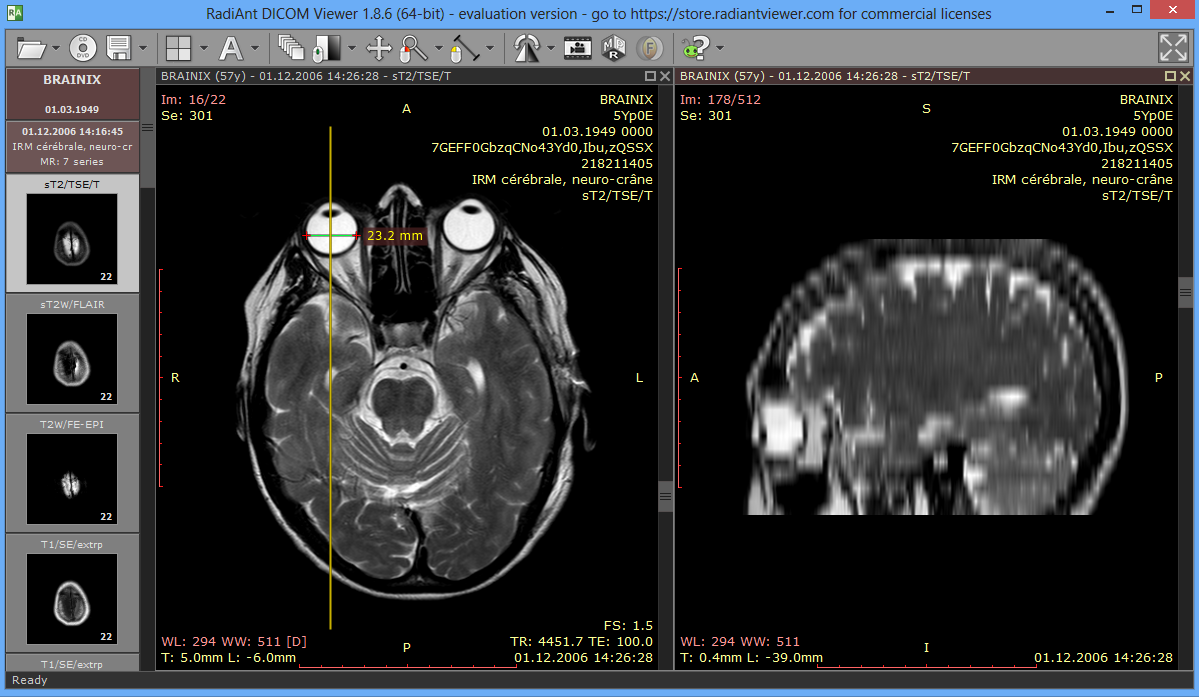
\includegraphics[angle=0,width=9cm]{./img/RadiAnt.png}}
   \caption{RadiAnt - DicomViewer}
  \label{radiant}
  \vspace{0.5cm}
\end{figure}

%\footnotetext{http://www.radiantviewer.com/de/}

% Jetzt eine gleitende Abbildung, die Abbildung wird am oberen 
% Seitenrand positioniert, die Fußnote erhält die Nummer 3
% Der Fußnotenbefehl wird nochmal geschützt

\section{Evaluierung bestehender Software}

Frei verfügbare Software im medizinischen Bereich beschränkt sich oft in den vom Programm vorgegebenen Funktionen und bietet keine Möglichkeit der Erweiterung. Zusätzlich liegt der Fokus auf der Darstellung der Patientenbilder und weniger an den Algorithmen zur Bildverarbeitung. Abbildung \ref{radiant} zeigt den Screenshot des DicomViewers RadiAnt\footnote{http://www.radiantviewer.com/de/}. Die Bilder können einzeln, oder wie auf dem Bild zu sehen, im Bezug zueinander betrachtet werden. Die Werkzeugleiste oben ermöglicht die für DICOM-Bilder typischen Operationen.
Zwar gibt es auf dem Markt auch Open-Source Lösungen mit Schwerpunkt auf Bildverarbeitung, jedoch eigenen sich diese nur bedingt für den Einsatz in der Lehre. Die Programme bieten eine Vielzahl an Funktionen, allerdings benötigt die Entwicklung von Erweiterungen einen erheblichen Zeitaufwand.
 
\begin{figure}[htbp]
  \vspace{0.5cm}
  \centering
  \fbox{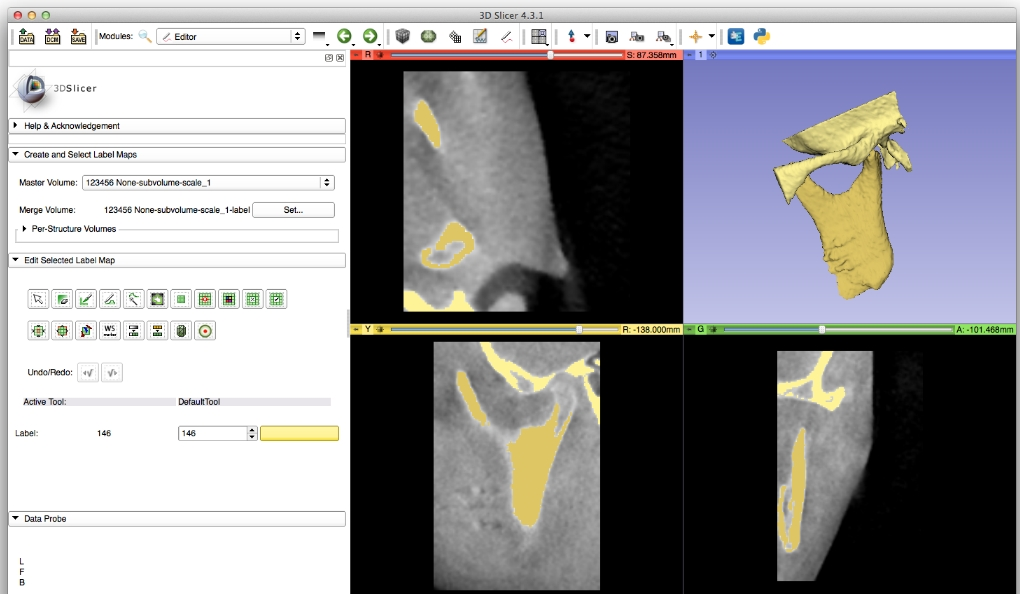
\includegraphics[angle=0,width=9cm]{./img/Screenshot-3DSlicer.png}}
  \floatfoot{Quelle: http://www.linuxlinks.com/portal/content/reviews/Health/Screenshot-3DSlicer.png - abgerufen am 11.01.2014}
  \caption{Screenshot Slicer 3D}
  \label{slicer3d}
  \vspace{0.5cm}
\end{figure}

\section{Slicer 3D}

Slicer 3D\footnote{http://www.slicer.org} (Abbildung \ref{slicer3d}) ist ein umfassendes Werkzeug für die medizinische Bildverarbeitung im zwei- und dreidimensionalen Raum. Die quelloffene Software bietet Möglichkeiten eigene Module zu implementieren. Slicer verwendet als Bibliotheken unter anderem das Insight Toolkit und das Visualization Toolkit\footnote{Insight Toolkit(ITK) und Visualization Toolkit (VTK) sind umfassende Programmbibliotheken zur medizinischen Bildverarbeitung und Visualisierung. Verfasst wurden sie in der Programmiersprache C++}. Das Modul \glqq medizinische Bildverarbeitung\grqq\ baut auf der Programmiersprache Java auf und ist eine weitere Voraussetzung für einen Einsatz im Lehrgebiet. Module in Slicer werden in Python implementiert. Die Studierenden müssten damit eine zusätzliche Sprache lernen.\\

\begin{figure}[htbp]
  \vspace{0.5cm}
  \centering
  \fbox{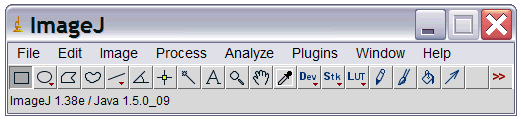
\includegraphics[angle=0,width=9cm]{./img/imagej-window.png}}
  \caption{Die Benutzeroberfläche von ImageJ}
  \floatfoot{ Quelle:  http://rsbweb.nih.gov/ij/features.html - abgerufen am 11.01.2014}
  \label{imagej}
  \vspace{0.5cm}
\end{figure}

\section{ImageJ}

ImageJ ist \glqq State Of The Art\grqq\ im Bereich der Bildverarbeitung in Java\footnote{http://rsbweb.nih.gov/ij/}). Im Grundzustand liefert ImageJ die Standardfunktionen der Bildverarbeitung wie Abbildung \ref{imagej} zeigt. Unter Anderem kann das Bildmaterial analysiert oder mit Filtern bearbeitet werden. ImageJ verarbeitet sowohl Grauwertbilder als auch Farbbilder in den gängigen Formaten wie PNG, JPEG und vielen Anderen. Mit Hilfe der \glqq ImageStacks\grqq\ ist auch eine Bearbeitung im dreidimensionalen Bildraum möglich. Erweiterungen können schnell und zielgerichtet entwickelt werden. Im Modul \glqq Bildverarbeitung\grqq\ der Fakultät Informatik wird ImageJ als Standard zum Bearbeiten der Übungsaufgaben verwendet. Für einen Einsatz im Studiengang Biomedizinische Technik fehlt allerdings die grundlegende Unterstützung von medizinischen Bilddaten im DICOM-Format. Die Funktionalität lässt sich über Plug-ins nachträglich hinzufügen, allerdings fehlt eine Bibliothek die bereits implementierte Algorithmen zur Verfügung stellt, sowie eine Verknüpfung von ImageJ-Klassen wie FloatProcessor oder ByteProcessor in Bildformate der Bibliotheken.

\section{Anforderungen}

Für eine Software die an der Hochschule Landshut für Lehre sowie Forschung im Bereich der medizinischen Bildverarbeitung eingesetzt werden kann ergeben sich folgende Anforderungen:

\begin{itemize}
\item \textbf{Erweiterbarkeit durch den Anwender} \\
	  Anwender sollen die Möglichkeit haben, das Programm mit selbst programmierten Algorithmen zu erweitern. Die eigene Implementierung von Bildverarbeitungsprozessen ist essentiell im Bereich der Lehre.
	  
\item \textbf{Interaktive Benutzereingaben}
	  Aus der Anwendererweiterbarkeit ergibt sich eine weitere Anforderung. Nicht immer können alle Eigenschaften und Werte der Algorithmen während der Implementierung vom Anwender bestimmt werden. Durch die Abhängigkeit von Bilddaten zu Algorithmen muss die Möglichkeit geboten werden, Parameter während der Laufzeit der Anwendung zu bestimmen. Zusätzlich müssen einzelne Bildpunkte interaktiv vom Benutzer ausgewählt und später von Algorithmen benutzt werden können.

\item \textbf{Anwendung der Algorithmen im dreidimensionalen Raum}\\
	  Eine Vielzahl an Bildaufnahmen liegen als dreidimensionaler Datensatz vor. Eine Reihe von Bildern muss folglich zusätzlich zur xy-Ebene auch in z-Richtung zu bearbeiten sein.

\item \textbf{Modularer Aufbau} \\
	  Die Software soll auch in den Grundfunktionen erweiterbar sein, die bei Auslieferung des Programms sofort zur Verfügung stehen (Skalierung, Rotation, etc.). Anders als die von Benutzern erstellten Plug-ins, die abhängig vom Anwender sind, muss eine Möglichkeit zur globalen Erweiterung gegeben werden.

\item \textbf{Unterstützung des Dicom-Standards}\\
	  Medizinische Bilddaten besitzen neben den rohen Pixeldaten noch eine Vielzahl zusätzlicher Information wie Patientendaten oder Seriennummern der Aufnahmen und benötigen eine spezielle Verarbeitung. Anders als übliche Grauwertbilder besitzen DICOM-Daten unter Anderem nicht 255 sondern bis zu $2^{16}$ verschiedene Grauwerte.

\item \textbf{Implementierung in der Programmiersprache Java}\\
	  Das Modul zur Bildverarbeitung der Biomedizinischen Technik findet in Java statt. Dadurch wird die Programmiersprache eine Anforderung, da ein Einsatz für die Lehre sonst nur erschwert möglich ist.

\item \textbf{Grundausstattung an medizinischen Bibliotheken}\\
	  Algorithmen in der Bildverarbeitung sind oft komplex und umfangreich. Nicht jeder benötigte Verarbeitungsprozess eignet sich zum selbst implementieren (Sowohl im Lehr- als auch Forschungsbereich). Durch den Einsatz von Bibliotheken wird ein grundlegender Satz an Algorithmen vorgegeben, auf den der Benutzer zurückgreifen und in den Plug-ins verwenden kann.
\end{itemize}

Da in den vorgestellten Anwendungen keine Lösung verfügbar ist, die alle Voraussetzungen erfüllt, soll eine Software entwickelt werden, die für das Labor für medizinische Bildverarbeitung, Algorithmen und Krankenhaus IT die benötigten Anforderungen erfüllt.

\chapter{Grundlagen medizinischer Daten- und Bildformate} \label{grundlagen}
\addthumb{Grundlagen der medizinischen Bildverarbeitung}{\huge{\textbf{\thechapter.}}}{white}{haw_rot}

\section{Bildgewinnung und bildgebende Verfahren}\label{grundlagen:bildgebung}

\section{DICOM}\label{grundlagen:dicom}
Der Name DICOM steht für \textit{Digital Imaging and COmmunication in Medicine}. Der Umgang mit diesem Standard ist essentieller Bestandteil der zu entwickelnden Software. Pianykh\cite{pianykh:dicom} beschreibt im ersten Kapitel, dass DICOM nicht nur aus Pixel und deren zugehörigen Werten besteht. Wie der Name sagt, ist auch die Kommunikation fest im Standard verankert. Damit ist die Übertragung der Daten von medizinischen Geräten(Modalitäten) zum zentralen Speicher und deren Verteilung gemeint. Des weiteren spielt die dauerhafte Speicherung der digitalen Aufnahmen eine große Rolle. Daher wird im gleichen Zug mit DICOM immer ein PACS genannt. Das Akronym PACS bedeutet \textit{Picture Archiving and Communication System} und besteht sowohl aus Hardware (Server, Speicherung) als auch Software(Verteilung und Kommunikation).\\
Abbildung \ref{communication} illustriert das Zusammenspiel des DICOM-Standards und dem zentralen Datenspeicher. Zuerst wird mittels der Modalitäten(z.B. mit dem Computertomographen oder einem Ultraschallgerät) die digitale Aufnahme erzeugt. Danach wird das Bild vom Gerät an das PACS gesendet. Hier werden die Aufnahmen und Patientendetails in die Datenbank und den Speicher abgelegt. Wird eine Aufnahme benötigt können Clients Anfragen mit beispielsweise dem Patientennamen stellen und erhalten die zugehörige Serie mit der digitalen Aufnahme.

\begin{figure}[htbp]
  \vspace{0.5cm}
  \centering
  \fbox{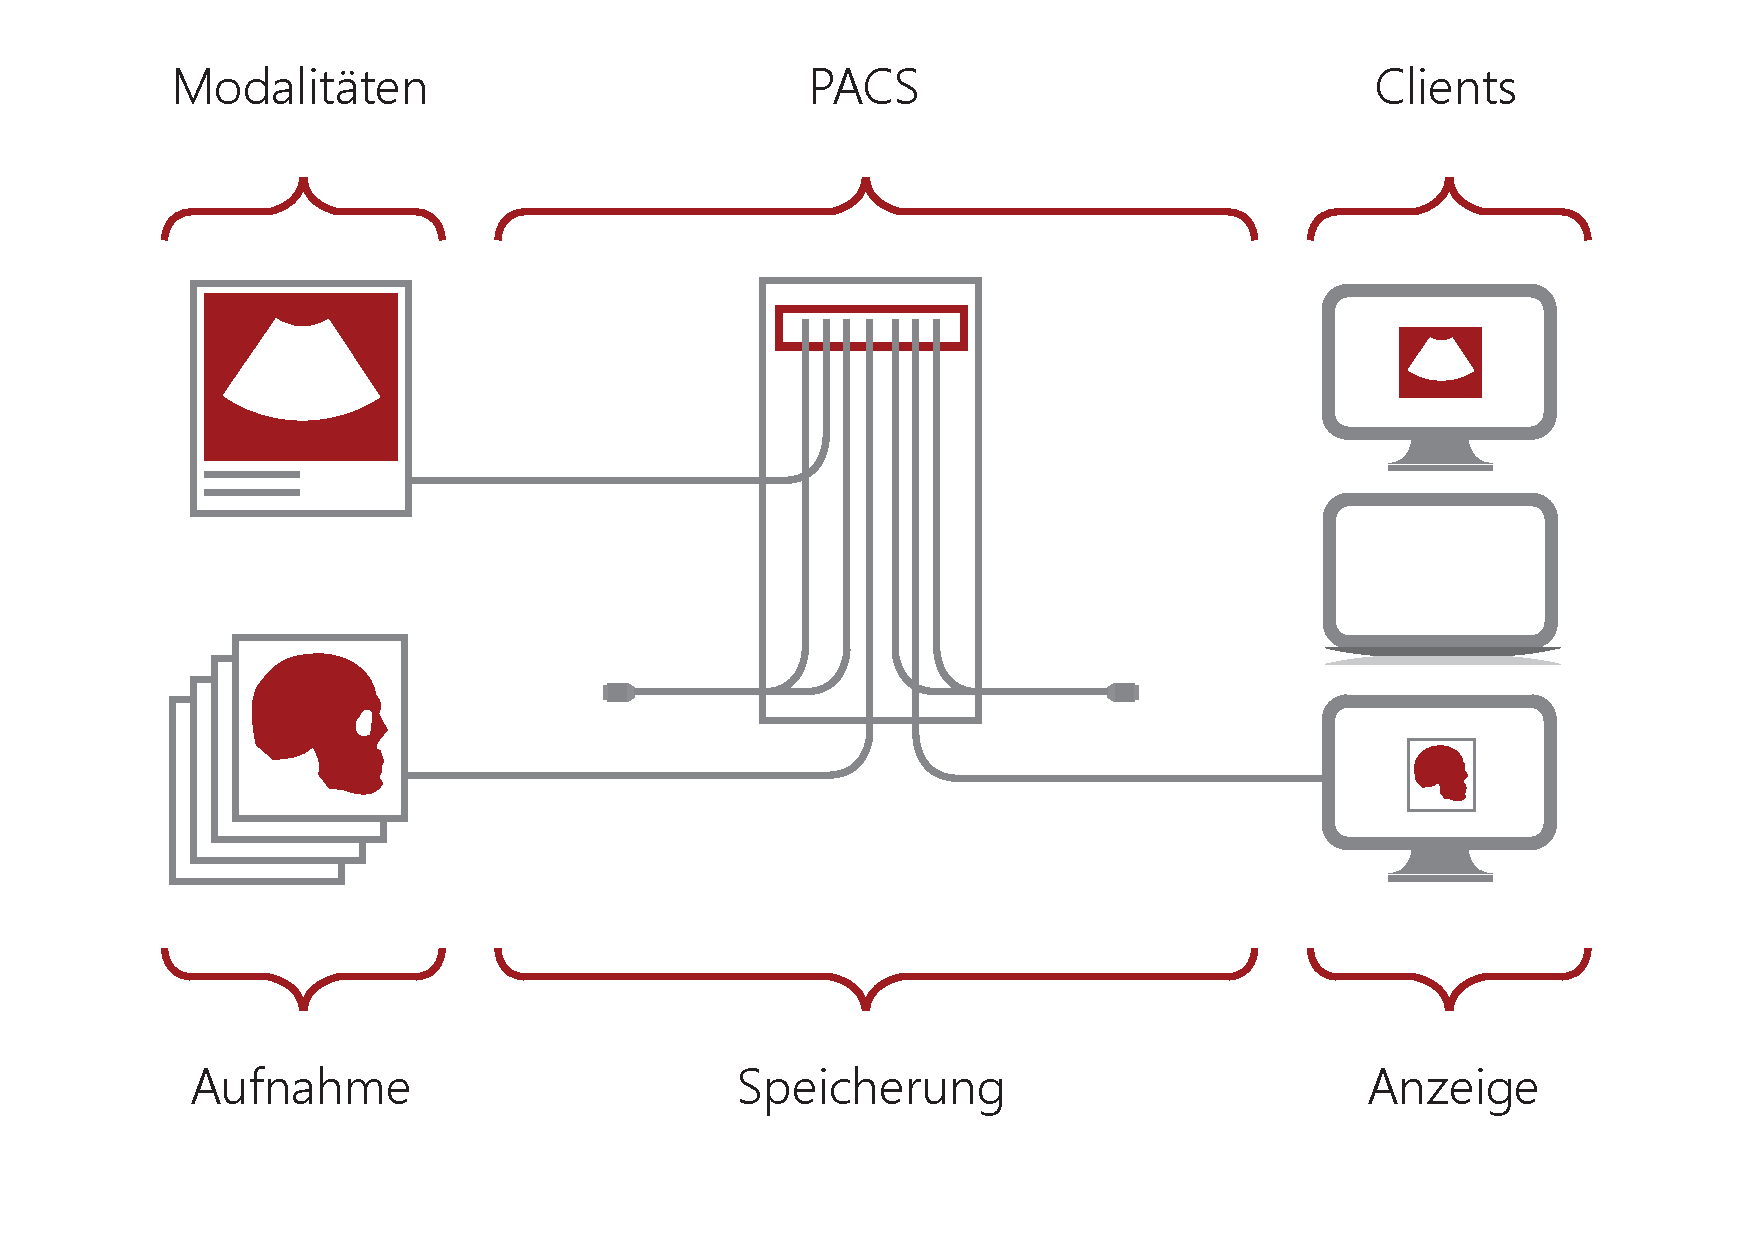
\includegraphics[angle=0,width=12cm]{./img/communication_neu.pdf}}
  \caption{Kommunikationsprozess von Aufnahme zur Verarbeitung}
  \floatfoot{Vorlage für diese Darstellung ist die Grafik in \cite[Fig. 1]{pianykh:dicom}}
  \label{communication}
  \vspace{0.5cm}
\end{figure}

DICOM\footnote{Unter ftp://medical.nema.org/medical/dicom/ lässt sich der aktuelle Standard abrufen. Die Kapitel befinden sich im Ordner zum jeweiligen Jahr der Veröffentlichung. Aktuell sind die Dokumente von 2011.} ist daher nicht nur ein einzelner Standard, sondern verknüpft die standardisierte 
\begin{itemize}
\item Kommunikation,
\item Erzeugung der Bilddaten,
\item und Speicherung.
\end{itemize}
Im Rahmen dieser Abschlussarbeit liegt der Fokus auf den Bilddaten, daher wird auf die Kommunikation- und Speicheraspekte nicht im Detail eingegangen.

\subsection{Die Dicom Information Object Definitionen} \label{grundlagen:iod}
Bevor die Pixeldaten genauer betrachtet werden können, muss der prinzipielle Aufbau der Dicomobjekte beschrieben werden. Teil 3 des Standards\cite[A.1.2]{dicom:iod} zeigt den relationalen Aufbau der Dicomobjekte. Vereinfacht können die elementaren Informationsobjekte in drei Teile aufgeteilt werden.

\begin{itemize}
	\item \textbf{Patient}\\
	Der Patient steht in der Hierarchie an oberster Stelle und ist die Grundlage für eine oder mehrere Studien(Study).
	\item	\textbf{Study}\\
	Study symbolisiert eine medizinische Studie. Eine Studie ist eine Sammlung von mehreren Serien, die von Modalitäten wie CT und MR aufgezeichnet werden. Eine Studie ist exakt einem Patient zugeordnet.
	\item \textbf{Series}\\
	Eine Serie ist ein Folge von Bildern, die von einer Modalität erzeugt wird. Die Aufnahmen eines CT werden einer Serie zugeordnet. Jede Serie gehört zu nur einer Studie.
	\item \textbf{Image, Real World Values}\\
	Auf der unteren Hierarchiestufe stehen Objekte wie Bilddaten oder die Lage des Patienten im Raum während der Aufnahme. Ein Bild wird genau einer Serie zugeordnet.
\end{itemize}

Aus diesen vier elementaren Objekten ergibt sich folgende Informationsstruktur für Dicomobjekte, die in Abbildung \ref{ermodel} als Entity-Relationship-Modell\footnote{Ein ER-Modell beschreibt die Beziehungen der Elemente zueinander. Dieser Diagrammtyp wird unter Anderem häufig beim Entwickeln der Struktur einer relationalen Datenbank verwendet} verdeutlicht wird.

\begin{figure}[htbp]
  \vspace{0.5cm}
  \centering
  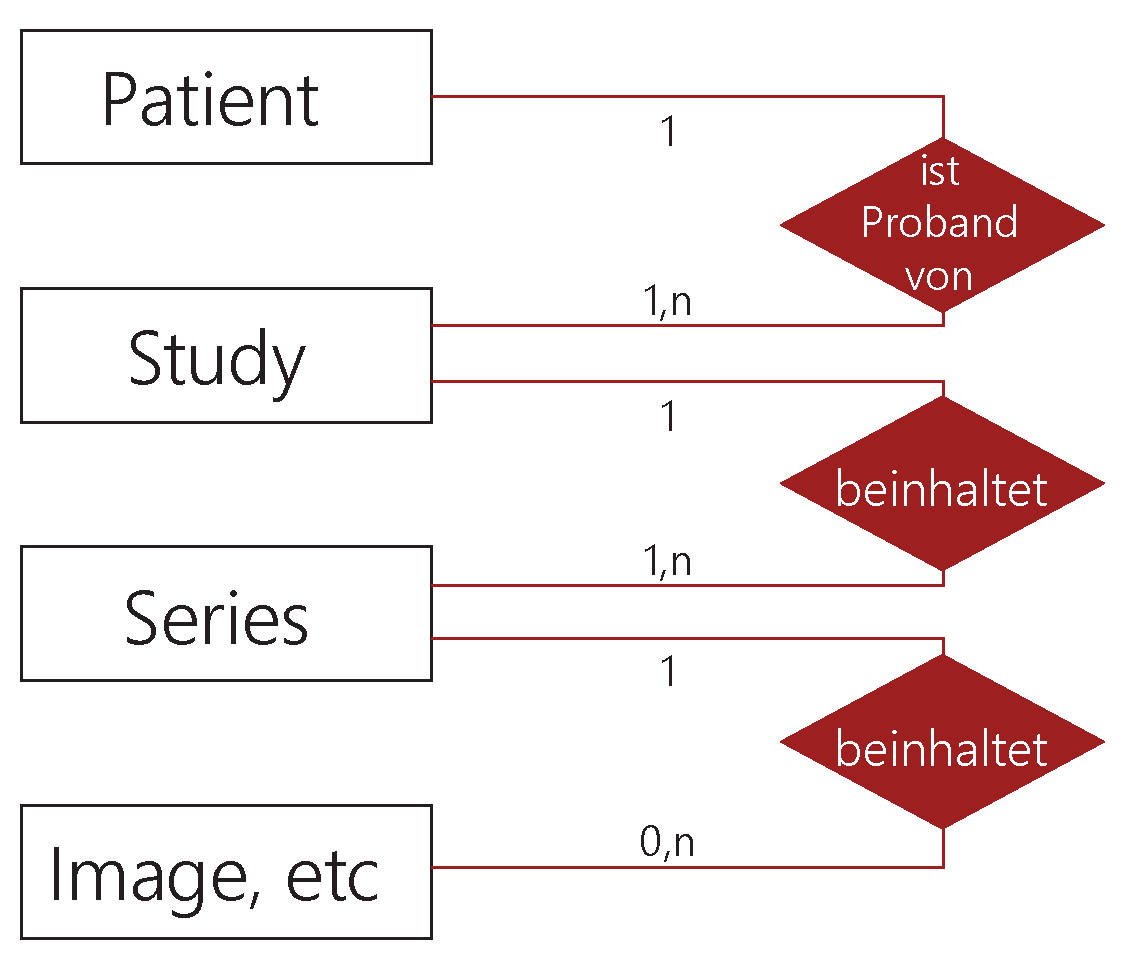
\includegraphics[angle=0,width=8cm]{./img/ermodel.pdf}
  \floatfoot{Vorlage für diese Darstellung ist die Grafik in \cite[A.1.2]{dicom:iod}}
  \caption{Vereinfachte Darstellung der Informationsobjekthierarchie von Dicomelementen}
  \label{ermodel}
  \vspace{0.5cm}
\end{figure}

Der DICOM-Viewer OsiriX bietet auf der Herstellerseite\footnote{http://www.osirix-viewer.com/datasets/} die Möglichkeit Testdaten zu beziehen. Betrachtet man die Repräsentation der Daten auf der Festplatte hält sich die Ordnerstruktur an obiges ER-Modell.\\
Abbildung \ref{filesystemrep} zeigt eine schematische Darstellung der Dateien. Die Beispieldaten von OsiriX bestehen aus einem Patient names \glqq Brebix\grqq\, dem eine Studie sowie zwei Serien à 100 Aufnahmen zugeordnet werden.

\tikzstyle{every node}=[draw=black,thick,anchor=west]
%\tikzstyle{selected}=[draw=red,fill=red!30]
\tikzstyle{optional}=[dashed,fill=gray!50]
\begin{figure}[htbp]
\centering
\caption{Repräsentation der Information Objekte im Dateisystem}
\label{filesystemrep}
\begin{tikzpicture}[%
  grow via three points={one child at (0.5,-0.7) and
  two children at (0.5,-0.7) and (0.5,-1.4)},
  edge from parent path={(\tikzparentnode.south) |- (\tikzchildnode.west)}]
  \node {Dicom Ordner}
    child [missing] {}
    child { node {BREBIX - Patient}
    	child [missing] {}
    	child { node{CT10 ponction foie - Studie}
    		child [missing] {}
    		child { node {DEF FOIE ART. - 107198 - Serie}
    			child{node[optional]{IM-0001-0001.dcm}}
    			child{node[optional]{...}}
    			child{node[optional]{IM-0001-0100.dcm}}
    		}
    		child [missing] {}				
    		child [missing] {}				
    		child [missing] {}
    		child [missing] {}
    		child { node {DEF. VEINEUX - 107205 - Serie}
    		    child{node[optional]{IM-0001-0001.dcm}}
    		    child{node[optional]{...}}
    		    child{node[optional]{IM-0001-0100.dcm}}
    		}
    		child [missing] {}
    	}
    };		
\end{tikzpicture}
\end{figure}

Bei näherem Hinsehen fällt auf, dass die Dateinamen beider Serien des Patienten identisch sind. Eine korrekte Zuordnung von DICOM-Dateien zur Serie ist daher nicht immer garantiert. Unabhängig von einer Repräsentation im Dateisystem oder Pfadangaben in der Datenbank eines PACS ist das Vertrauen auf Dateipfade unsicher, da über eine einfache Dateimanipulation die Zuordnung nicht mehr hergestellt werden kann.\\
Um eine zuverlässige Verknüpfung zu gewährleisten besitzt jeder Patient\footnote{Die Identifikationsnummern von Patienten sind meist nur innerhalb einer Institution oder Krankenhauses einzigartig, da diese manuell vergeben werden können\cite[5.6.2]{pianykh:dicom}.}, jede Studie und jede Serie eine Eindeutige Identifikationsnummer. Diese Art der Informationen wird in den einzelnen Dateien mit Hilfe von Einträgen aus dem DICOM Data Dictionary\cite{dicom:dd} hinterlegt. Die DICOM-Dateien beschreibt Pianykh \cite[S. 47]{pianykh:dicom}
als eine Kopie im Speicher vom tatsächlichen DICOM-Objekt.

\subsection{Der Transfer vom Patienten zu digitalen Dicomobjekten} \label{grundlagen:dicomObjects}
Wie der Name bereits andeutet ist das DICOM Data Dictionary vergleichbar mit einem Wörterbuch. Es enthält alle gültigen Elemente, die zur Beschreibung eines DICOM-Objekts verwendet werden können. Zusätzlich zu dem aus dem Standard bekannten Vokabular können Hersteller medizinischer Geräte ein eigenes Dictionary hinzufügen. Die proprietären Elemente können allerdings nicht standardisiert verarbeitet werden(vgl. \cite[S.45]{pianykh:dicom}, da Software die diese Objekte verarbeitet, nichts von der Existenz dieser Elemente weiß).\\
Mit Hilfe des Wörterbuchs und den ca. 2000 enthaltenen Daten können nun Aussagen des wirklichen Lebens (vorausgesetzt die Aussage ist mit einem Element aus dem Wörterbuch darstellbar) ins Digital übersetzt werden.\\
Tabelle \ref{table:patientname} zeigt das DICOM-Element für den Namen des Patienten aus dem Data Dictionary\cite[S. 14]{dicom:dd}.

\begin{table}
    \begin{tabularx}{\textwidth}{|X|X|X|X|X|}
    \toprule
    \hline
    \textbf{Tag}         & \textbf{Tagname}     & \textbf{VR} & \textbf{Wert}     	& \textbf{VM} \\ \hline
    (0010,0010) 		 & PatientName 			& PN 		  & John\^{}Doe 		& 1  \\  \hline
    \bottomrule
    \end{tabularx}
    \caption {Repräsentation des Patientennamen als DICOM-Element}
    \label{table:patientname}
\end{table}

Betrachtet man den folgenden Satz(vgl. \cite[S.46]{pianykh:dicom}), kann dieser in ein DICOM-Object, wie es Tabelle \ref*{table:translation} darstellt, übersetzt werden:
\begin{center}
\textit{\glqq John Doe, männlich, geboren am 01. Januar 1970\grqq}
\end{center}

Aus den Beispielen von Tabelle \ref{table:patientname} und \ref{table:translation} lässt sich erkennen, dass ein DICOM-Element nochmals in atomare Teile aufgespalten werden kann. Folglich besteht ein Datenelement aus einem beschreibenden \textit{Tag}, einer \textit{VR(Value Representation)}, einem Wert und der \textit{VR (Value Multiplicity)}. Das Element selbst nimmt eine von drei Darstellungsmöglichkeiten ein. Zusätzlich liegt im Speicherabbild des Datenelements die Länge des Wertes\footnote{John\^{}Doe besitzt aufgrund der Zeichenmenge eine Länge von acht}. Abhängig von der Transfersytax\footnote{Unter der Transfersystax verstehn man eine Menge an Kodierungsvorschriften von DICOM-Objekten\cite[S.63 Section 10]{dicom:structure}. Zu diesen Vorschriften gehört zum Beispiel die Reihenfolge der Bytes im DICOM-Element oder die Komprimierung der Bilddaten} des DICOM-Objekts ist der VR-Teil optional. Die weiteren beiden Darstellungen unterscheiden sich in der Kodierung der benötigten Länge des Werts \cite[7.1]{dicom:structure}.  Anhang \ref{appendix:speicher} auf Seite \pageref{appendix:speicher} zeigt wie Datenelemente im Speicher abgelegt werden und wie viel Speicherplatz pro Element reserviert werden muss.

\begin{table}
    \begin{tabularx}{\textwidth}{|p{4cm}|p{4cm}|X|X|X|}
    \toprule
    \hline
    \textbf{Tag\newline \small{(Gruppe, Element)}}         & \textbf{Tagname}     & \textbf{VR} & \textbf{Wert}     	& \textbf{VM} \\ \hline
    (0010,0010) 		 & PatientName 			& PN 		  & John\^{}Doe 		& 1  \\ \hline
    (0010,0030) 		 & PatientBirthDate		& DA 		  & 19700101	 		& 1  \\ \hline
    (0010,0040)			 & PatientSex 			& CS 		  & M			 		& 1  \\ \hline
    (0010,1010) 		 & PatientAge 			& AS 		  & 44			 		& 1  \\ \hline
    \bottomrule
    \end{tabularx}
    \caption {Das erzeugte DICOM-Objekt mit den Elementen zu Patientenname, Geburtsdatum, Geschlecht und Alter}
    \label{table:translation}
\end{table}

\subsection{Tags in Datenelementen}

Ein DICOM-Element wie PatientName kann über ein Tag identifiziert werden. Ein Tag ist in einem DICOM-Objekt einzigartig und darf nur ein mal benutzt werden. Die numerische Darstellung hat die Form (\textit{gggg}, \textit{eeee}) wobei die hexadezimalen Ziffern \textit{g} die Gruppe des DICOM-Elements beschreiben und \textit{e} das Element der Gruppe \textit{g} definiert. Zusätzlich zu diesen Eigenschaften, kann bestimmt werden, ob der Ursprung eines DICOM-Elements im Standard- oder einem privaten Data Dictionary liegt. Eine gerade Gruppen-Ziffer zeigt, dass das Element Teil des Standards ist während ungerade für proprietäre Elemente stehen\footnote{Ausgenommen aus dieser Regel sind folgende Gruppen: (0000, eeee), (0002, eeee), (0004, eeee), (0006, eeee), (0001, eeee), (0003, eeee), (0005, eeee), (0007, eeee), (FFFF, eeee)}\cite[7.1]{dicom:structure}. Die Reihenfolge der Tags ist in numerischer Folge in aufsteigender Form sortiert. Fällt während des Einleseprozesses in eine Datei auf, dass die Reihenfolge nicht korrekt ist, deutet dies auf ein korruptes DICOM-Objekt hin.\\

\subsection{VR - Value Representation}
Dieser Teil eines DICOM-Elements beschreibt den Typ und das Format des Wertes\cite[6.2]{dicom:structure}. Der Umfang an verschiedenen Value Representations reicht von Zeichenketten wie PersonName (PN) im Datenelement (0010,0010) PatientName über Datumsangaben (DA) bis zu numerischen Werten(FL) und Sequenzen (SQ). Eine vollständige Liste ist im Standard unter \cite[Table 6.2.1]{dicom:structure} zu finden.\\
Zwecks Vollständigkeit soll erwähnt werden, dass ein Datenelement mit VR-Typ SQ wiederum ein DICOM-Object enthalten kann und dadurch eine Baumstruktur entsteht.

\subsection{VM - Value Multiplicity}
Value Multiplicity bestimmt die Anzahl an Werten, die in einem DICOM-Element enthalten sind. Die Werte werden durch einen Backslash \textbackslash voneinander getrennt. Der explizite Wert der Value Multiplicity kann aus dem Data Dictionary entnommen werden.\cite[6.4]{dicom:structure}

\section{DICOM Pixeldaten und Bildformate}

Die Abschnitte \ref{grundlagen} - \ref{grundlagen:dicomObjects} zeigen, dass DICOM mehr als ein Bildformat darstellt, ein essentieller Bestandteil bleiben jedoch die Pixel eines DICOM-Objekts (auch wenn diese nur optional vorhanden sein müssen, wie Grafik \ref{ermodel} zeigt). Nach dem DICOM Data Dictionary gehören Bild-abhängige Informationen zur Gruppe (\textit{0028}, \textit{eeee}).
Die Pixeldaten liegen im Bereich (\textit{7fe0}, \textit{0010}) am Ende eines DICOM-Objekts.\\
Das bedeutet, dass die konkreten Werte der Pixel im gleichen DICOM-Objekt liegen und den selben Kodierungsrichtlinien der DICOM-Tags unterliegen.

\subsection{Kodierung der Pixel im Speicherabbild eine DICOM-Objekts} \label{pixelkodierung}

Um die grundlegende Struktur der Pixel im DICOM-Objekt zu beschreiben sind drei Datenelemente notwendig: BitsAllocated, BitsStored und HighBit\ref{table:digitalRep}. BitsAllocated beschreibt, wie viel Speicher für einen singulären Pixelwert reserviert wird. Mit Hilfe von Columns und Rows kann die Bilddimension bestimmt werden. Columns beschreibt die Breite, Rows die Höhe. Die Value Representation des Datenelements PixelData (\textit{7fe0}, \textit{0010}) kann nach DICOM Data Dictionary entweder den Wert \textit{OB} oder \textit{OW} annehmen. OB bedeutet \textit{Other Byte String} während OW für \textit{Other Word String} steht. Nach Section 8.1 des Standards\cite{dicom:structure} besteht der Unterschied zwischen den beiden VRs darin, dass OB abhängig von der Byteordnung ist. Ob die Ordnung Little Endian oder Big Endian entspricht ist abhängig von der Transfersyntax des DICOM-Objekts.
Grafik \ref{byteorder} zeigt die Kodierungsreihenfolge. Little Endian kodiert vom Least Significant Bit (LSB) zum Most Significant Bit (MSB). Big Endian verarbeitet die Byte in umgekehrter Reihenfolge. Ein Element von PixelData (sowohl mit einer VR von OB als auch OW) fasst 16 Bit, was gleichzeitig die maximale Größe an allokiertem Speicher von BitsAllocated darstellt.

\begin{figure}[htbp]
  \vspace{0.5cm}
  \centering
  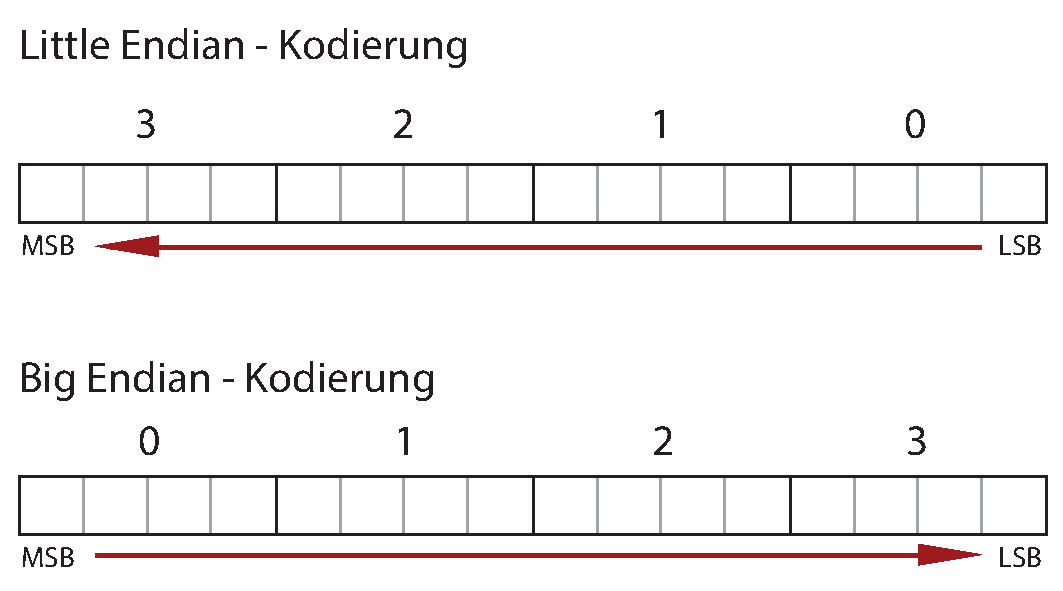
\includegraphics[angle=0,width=10cm]{./img/byteorder.pdf}
  %\floatfoot{Vorlage für diese Darstellung ist die Grafik in \cite[A.1.2]{dicom:iod}}
  \caption{Kodierungsreihenfolge von 4 Byte bei Little Endian- und Big Endian-Darstellung}
  \label{byteorder}
  \vspace{0.5cm}
\end{figure}

BitsStored gibt darüber Auskunft, wie viel Bit pro Wert in Anspruch genommen werden. Schließlich gibt HighBit das in der Reihenfolge ranghöchste Bit von StoredBits an \cite[8.1.1]{dicom:structure}.\\
Abbildung \ref{bits:pixel} verdeutlicht die Repräsentation eines Pixels im Datenelement PixelData. Die Darstellung entspricht einem eindimensionalen Array. Das erste Element ist das erste Pixel in der linken oberen Ecke, das letzte Element stellt den Pixel rechts unten dar. \ref{bits:16} und \ref{bits:8} zeigen die exakte Belegung an Bit bei BitsStored 16 und BitsStored 8. Der graue Hintergrund zeigt die allokierten Bit, während der rote Bereich den tatsächlich benutzten Speicher markiert. Der Pixelwert in Abbildung \ref{bits:8} nimmt den gesamten Speicherplatz pro Pixel ein. Das schwarze Quadrat steht für das HighBit.\\
Das Intervall der Werte ist abhängig von der Anzahl an gespeicherten Bits. Hat das Element StoredBits den Wert 12 kann ein  Pixel einen Wert aus dem Bereich von $[0, 2^{12}-1]$ annehmen. Entspricht StoredBits 8 ist das Intervall $[0, 2^8-1]$. Hier spricht man von einer Grauwerttiefe von 12 beziehungsweise 8 \cite[2.2]{handels:mbv}.
\begin{figure*}[htb]
%\subfigure[Keypoints]{\includegraphics[width=0.49\textwidth]{./img/basmati_keypoints.png}}\hfill
\centering
\fbox{
\subfigure[Pixel im Speicher]{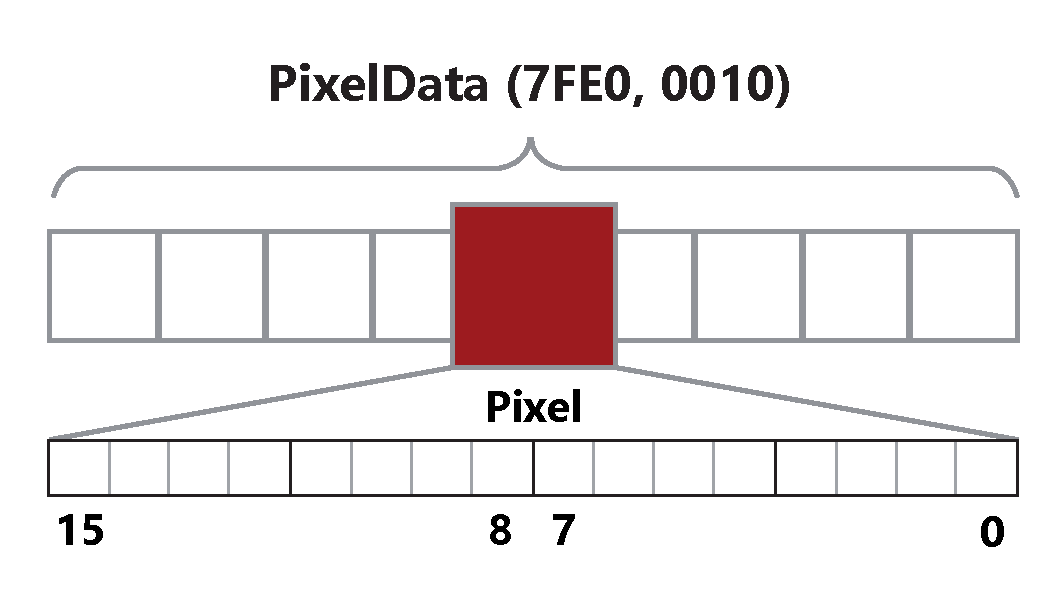
\includegraphics[width=5cm]{./img/bits.pdf} \label{bits:pixel}}
\subfigure[BitsAllocated 16, BitsStored 12, HighBit 11]{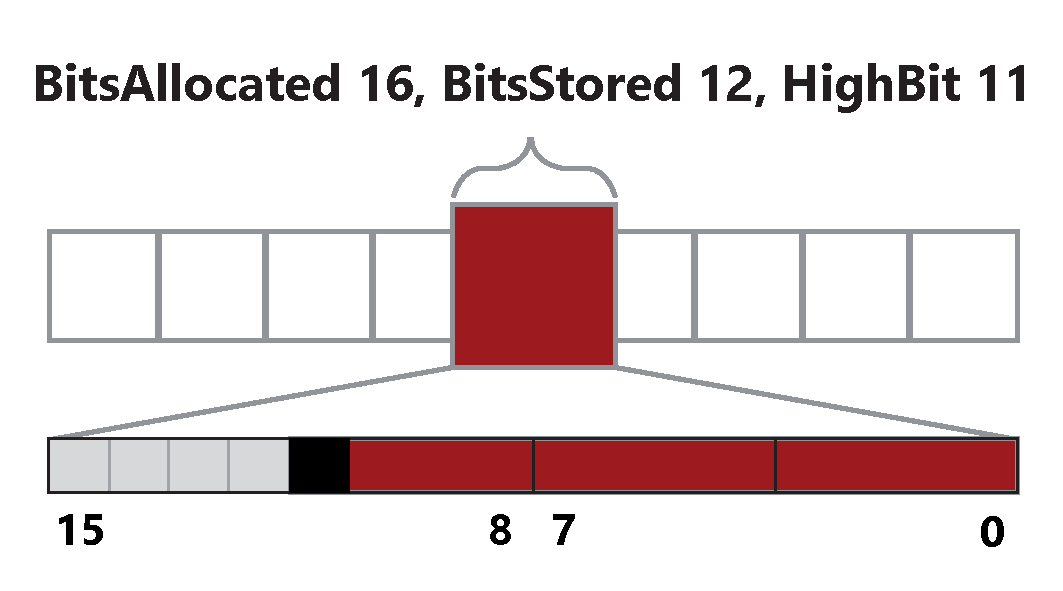
\includegraphics[width=5cm]{./img/bits16.pdf} \label{bits:16}}
\subfigure[BitsAllocated 8, BitsStored 8, HighBit 7]{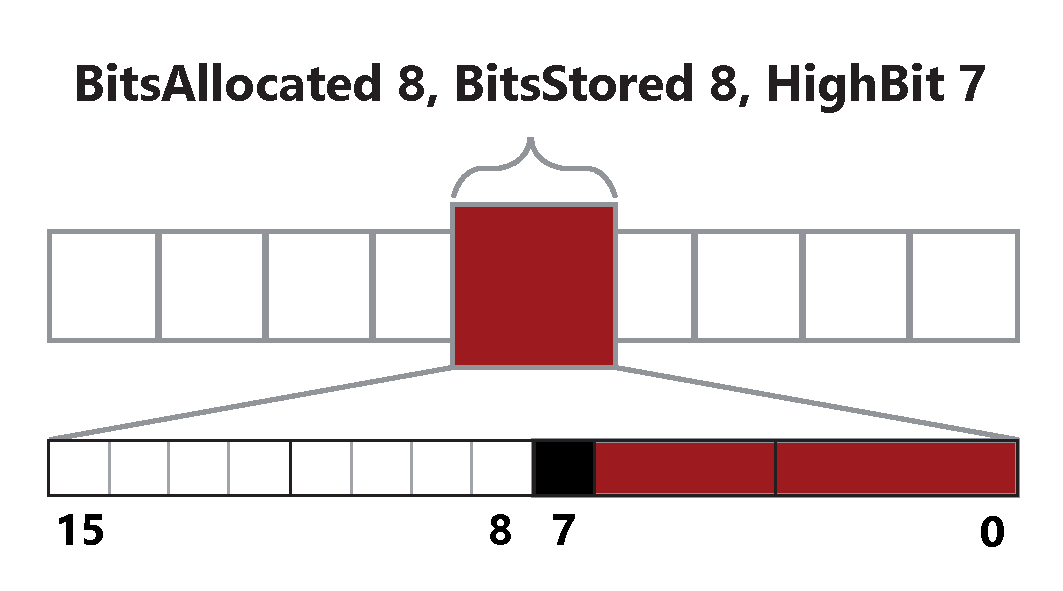
\includegraphics[width=5cm]{./img/bits8.pdf} \label{bits:8}}
}
\caption{Beispiele unterschiedlicher Speicherbelegung}
\label{bits}
\end{figure*}

Verschiedene Datenelemente aus dem DICOM-Standard liefern nähere Informationen zum Bildformat. So gibt das Element SamplesPerPixel (0028,0002) Auskunft darüber, wieviel Teile aus PixelData ein einzelnes Pixel repräsentieren. Hat Samples den Wert 1, so ist jedes Element aus PixelData genau ein Pixel. Daraus folgt, dass ein Grauwertbild vorliegt. 3 bedeutet, dass im DICOM-Objekt ein Farbbild mit den drei Kanälen rot, grün und blau liegt.\\
Die Werte der Pixel sind stark abhängig vom medizinischen Gerät, welches die Bilder aufzeichnet. Ein direkter Vergleich von Bildern, die von unterschiedlichen Geräten einer Modalität aufgezeichnet wurden ist daher nicht möglich. Um Gewebestrukturen von beispielsweise CT-Aufnahmen trotz dieser Abhängigkeiten patienten- und geräteübergreifend zu vergleichen, gibt es unter Anderem die Hounsfield Skala \cite[2.1.3]{handels:mbv}. Mit Hilfe der Datenelemente RescaleSlope und RescaleIntercept lassen sich die ursprünglichen Werte in brauch- und lesbare Pixelwerte konvertieren. RescaleType gibt die Skala an, mit der das Ergebnis interpretiert werden kann. Ein Umrechnung erfolgt mit der Formel aus \cite[C.11-1b Seite 1168]{dicom:iod}\\

\begin{equation}
Output=m*SV+b
\label{rescale}
\end{equation}

mit $m = RescaleSlope$, $b = RescaleIntercept$ und $SV=Pixelwert$.

Fettgewebe zum Beispiel nimmt nach der Hounsfield-Skala Werte zwischen 0 und -100 ein \cite[Abbildung 1.18 Seite 15]{radio:hounsfield}. Ob in einem DICOM-Objekt vorzeichenbehaftete Werte vorhanden sind, sagt das Element PixelRepresentation. Eine 0 bedeutet kein Vorzeichen. Bei einem Wert von 1 können negative Werte enthalten sein.
\begin{table}
    \begin{tabularx}{\textwidth}{|X|X|X|}
    \toprule
    \hline
    \textbf{Tag}         & \textbf{Tagname}     & \textbf{VR} \\ \hline
    (0028,0010) 		 & Rows					& US 		  \\ \hline
    (0028,0011) 		 & Columns				& US 		  \\ \hline
    (0028,0100) 		 & BitsAllocated		& US 		  \\ \hline
    (0028,0101) 		 & BitsStored			& US 		  \\ \hline
    (0028,0102)			 & HighBit				& US 		  \\ \hline
    \bottomrule
    \end{tabularx}
    \caption {Grundlegende Datenelemende für die digitale Repräsentation}
    \label{table:digitalRep}
\end{table}

\subsection{Grauwertbilder} \label{grey_images}

Für Bildverarbeitungsprozesse und Algorithmen bieten Grauwertbilder einige Vorteile im Vergleich zu Farbbildern. Der größte Unterschied liegt beim Verhältnis zwischen Informationsgehalt zu Speicherbedarf. Farben bieten bei Kantenübergängen oder Helligkeitsinformationen keinen Mehrwert. Das führt unter Anderem dazu, dass Industrie oder auch die medizinische Bildverarbeitung vorwiegend auf dieses Format zurückgreifen.\\
Eine Grauwerttiefe von 8 Bit ist Standard in der Bildverarbeitung. Das entspricht dem Intervall von $[0,255]$ und den Werten, die mit handelsüblichen Monitoren darstellbar sind. Medizinische Bilddaten können, wie in Abschnitt \ref{pixelkodierung} beschrieben, eine Tiefe von bis zu 16 Bit annehmen und Grauwerte aus dem Bereich $[0,65535]$ repräsentieren.

\begin{figure*}[htb]
%\subfigure[Keypoints]{\includegraphics[width=0.49\textwidth]{./img/basmati_keypoints.png}}\hfill
\centering
\fbox{
\subfigure[CT]{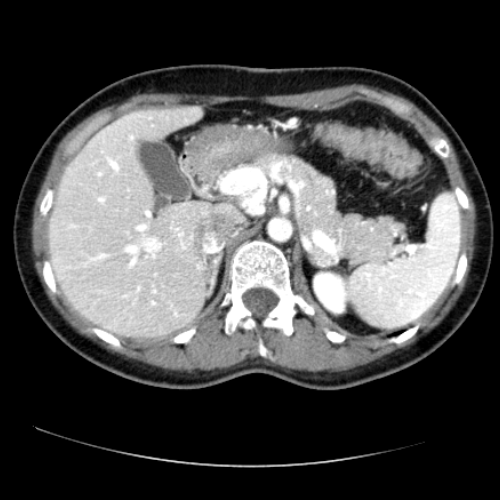
\includegraphics[width=5cm]{./img/ct.png} \label{ct}}
\subfigure[MR]{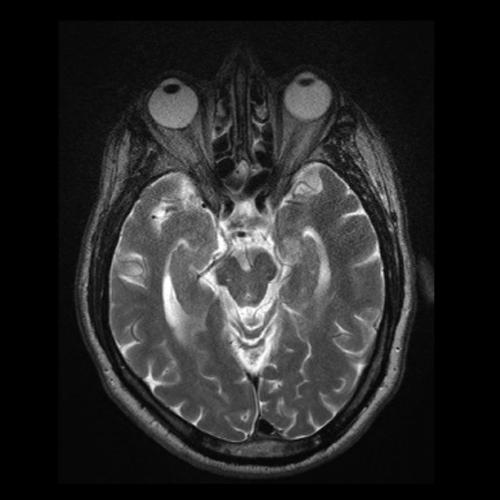
\includegraphics[width=5cm]{./img/mr.png} \label{mr}}
\subfigure[Ultraschall]{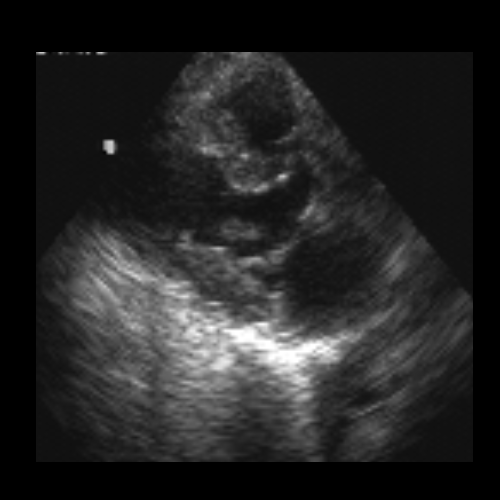
\includegraphics[width=5cm]{./img/sono.png} \label{sono}}
}
\floatfoot{Die Beispieldaten stammen von http://www.osirix-viewer.com/datasets/ - abgerufen am 19.01.2014}
\caption{Verschieden Graustufenbilder}
\label{grey}
\end{figure*}

\subsubsection{Fensterung von Grauwerten} \label{windowing}

Wie bereits in \ref{grey_images} beschrieben, lassen sich auf üblichen Monitoren nicht alle Grauwerte zur gleichen Zeit anzeigen. Dadurch müssen die maximal 65535 verschiedenen Grauwerte auf 255 abgebildet werden können. Dies wird durch die in der Radiologie verwendete Fensterungstechnik möglich\cite[Kapitel 8, Seite 249]{handels:mbv}. Es wird ein Fensterzentrum und eine Fensterbreite gewählt. Alle Werte innerhalb dieses Intervalls werden zwischen 0 und 255 umgerechnet. Abbildung \ref{window_graph} verdeutlicht dieses Prinzip. Ein CT-Bild mit einer Tiefe von 12 Bit besitzt 4096 Grauwerte. Ein Zentrum von 2000 und eine Breite von 500 bildet alle Werte von 1750 bis 2250 auf 0 bis 255 ab. Ist ein Pixeldatum kleiner 1750 wird das Minimum 0 hinterlegt und ist der Wert größer 2250 bekommt das Pixel das Maximum 255.\\
Im DICOM-Standard ist ein Algorithmus gegeben, um die Pixeldaten zu konvertieren\cite[C.11.2.1.2]{dicom:iod}.

\begin{algorithm}
\caption{Berechne den Fensterungswert aus originalem Pixelwert}
\begin{algorithmic}[1] 
\STATE $X \leftarrow input$ - tatsächlicher Pixelwert
\STATE $Y \leftarrow output$ - konvertierter Wert zwischen 0 und 255
\STATE $C \leftarrow windowCenter$
\STATE $W \leftarrow windowWidth$
\IF{$X <= C - 0.5 - (W-1)/2$}
	\STATE  $Y = Y_{min}$
\ELSIF {$X > C - 0.5 + (W-1)/2$}
	\STATE $Y = Y_{max}$
\ELSE
	\STATE $Y = ((X-(C-0.5)) / (W-1)+0.5)*(Y_{max}-Y_{min})+Y_{min}$
\ENDIF
\end{algorithmic}
\end{algorithm}


\begin{figure*}[htb]
%\subfigure[Keypoints]{\includegraphics[width=0.49\textwidth]{./img/basmati_keypoints.png}}\hfill
\centering
\fbox{
\subfigure[Fensterungstechnik]{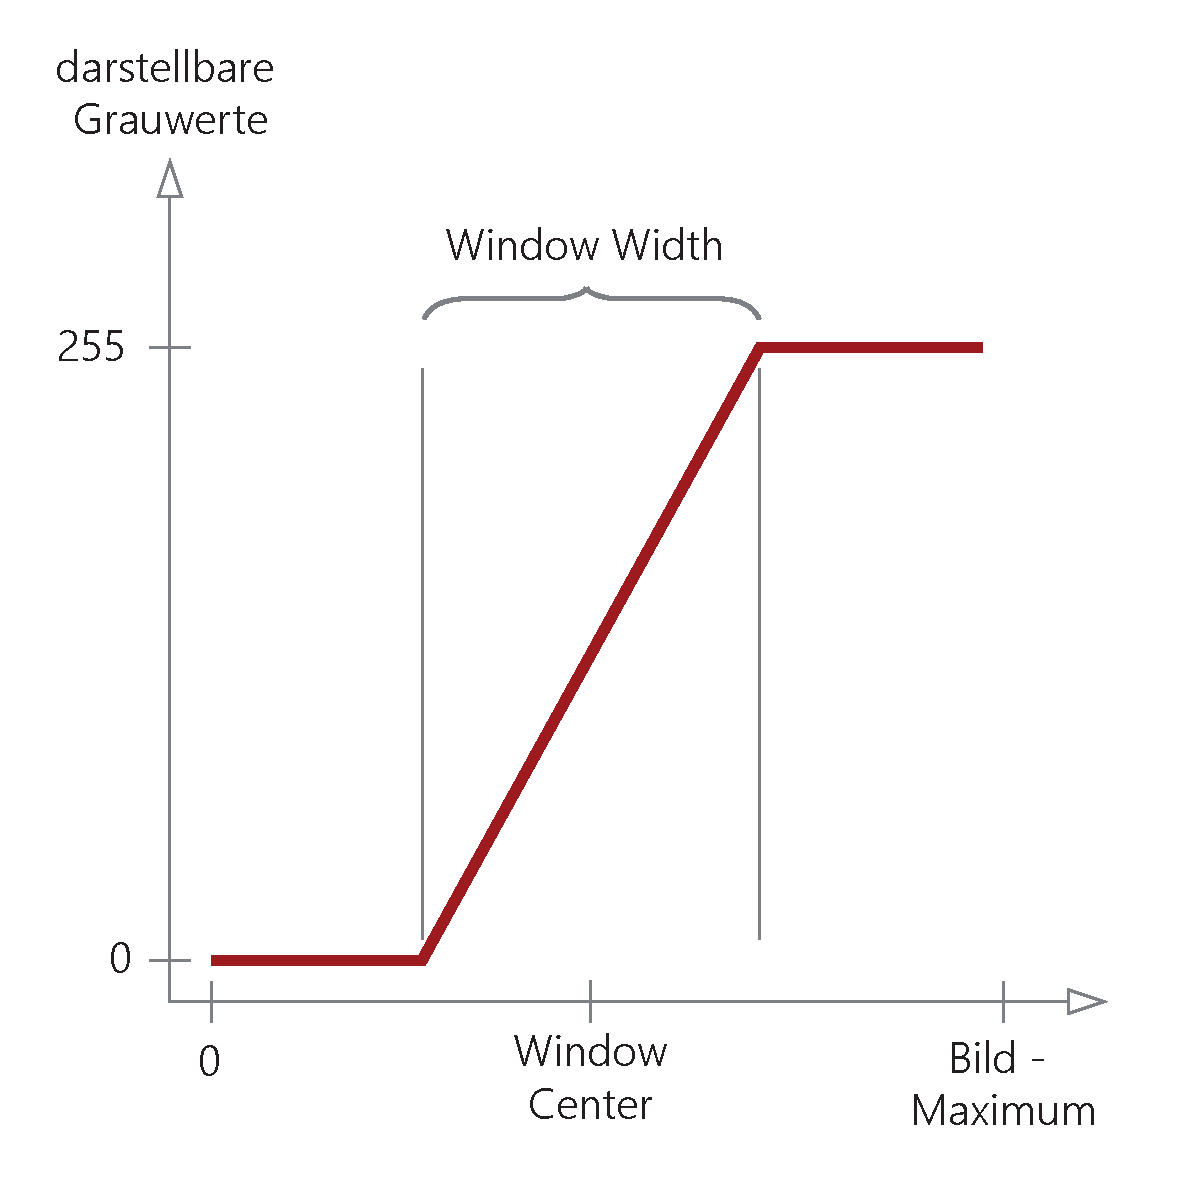
\includegraphics[width=5cm]{./img/fensterung.pdf} \label{window_graph}}
\subfigure[Window Center 50; Window Width 350]{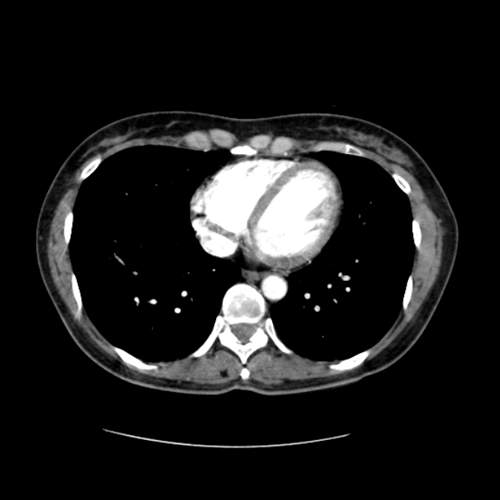
\includegraphics[width=5cm]{./img/window_a.png} \label{window_a}}
\subfigure[Window Center -124; Window Width 3134]{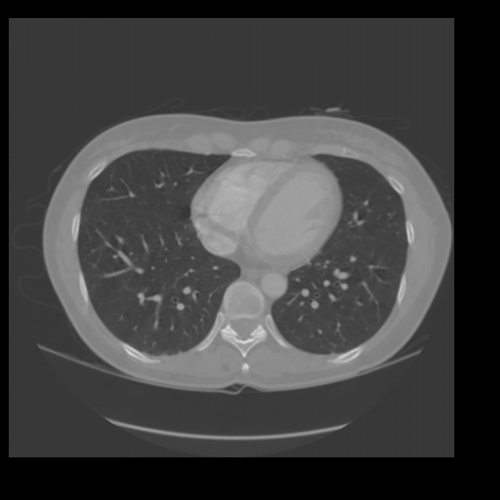
\includegraphics[width=5cm]{./img/window_b.png} \label{window_b}}
}
\floatfoot{Vorlage für die Grafik der Fensterungstechnik ist\cite[Abbildung 8.1]{handels:mbv}; Die Beispieldaten stammen von http://www.osirix-viewer.com/datasets/ - abgerufen am 19.01.2014}
\caption{Fensterungstechnik zur Darstellung medizinischer Bilddaten am handelsüblichen Monitor}
\label{window_sub}
\end{figure*}

\subsection{Farbbilder} \label{color_images}
Obwohl Grauwertbilder das am meisten verwendete Format in der medizinischen Bildverarbeitung darstellen, haben auch Farbbilder die verschiedensten Einsatzgebiete. So wird in der Dermatologie auf Farbdarstellungen zurückgegriffen um Hauterkrankungen zu dokumentieren\cite[2.2.3.2]{handels:mbv}. Des weiteren kann mit Farbultraschallbildern die Fließrichtung und Geschwindigkeit des Blutes visualisiert werden und dienen zur Untersuchung von Venen und Arterien\footnote{http://www.diagnostikum-berlin.de/farbkodierte-duplexsonographie-fkds - abgerufen am 19.01.2014}.\\
Wie bereits beschrieben, ist das Datenelement SamplesPerPixel mit einem Wert von drei der Indikator, dass ein Farbbild vorliegt. Das bedeutet pro Pixel werden 3 Elemente von PixelData belegt mit je einem Element für den roten, grünen und blauen Farbkanal. Daraus resultiert der dreifach Speicherbedarf, $BitsAllocated * SamplesPerPixel$ \cite[C.7.6.3.1.1]{dicom:iod}. Der DICOM-Standard bietet zwei Möglichkeiten, wie diese Information im Speicher hinterlegt werden. Entweder werden die Pixelwerte fortlaufend gespeichert mit R1, G1, B1; R2 ,G2, B2; ...RN, GN, BN; oder nach dem Kanal R1, R2, ...RN; G1, G2, ...GN; B1, B2, ...BN \cite[C.7.6.3.1.3]{dicom:iod}. Das Element dazu aus dem Data Dictionary heißt PlanarConfiguration(0028,0006). Abbildung \ref{planar} macht die beiden Schemata deutlich.

\begin{figure*}[htb]
%\subfigure[Keypoints]{\includegraphics[width=0.49\textwidth]{./img/basmati_keypoints.png}}\hfill
\centering
\fbox{
\subfigure[PlanarConfiguration = 0]{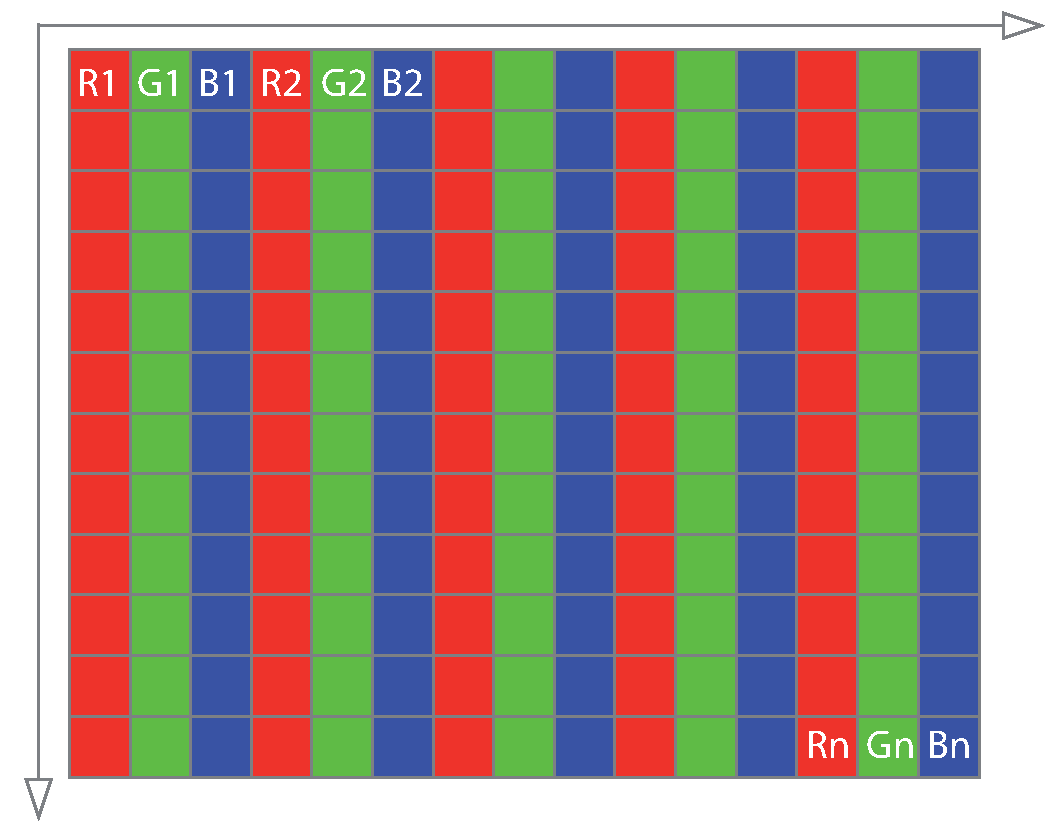
\includegraphics[width=8cm]{./img/planar_b.pdf} \label{planar_a}}
\subfigure[PlanarConfiguration = 1]{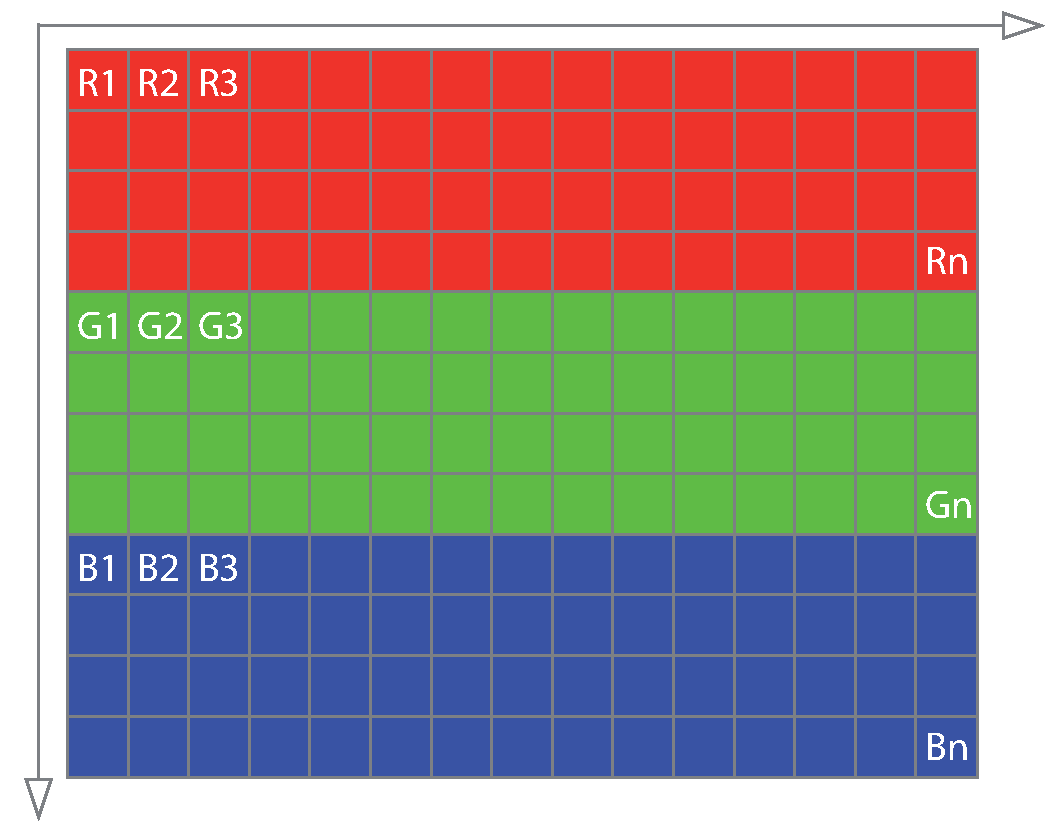
\includegraphics[width=8cm]{./img/planar_a.pdf} \label{plaanr_b}}
}
%\floatfoot{Vorlage für die Grafik der Fensterungstechnik ist\cite[Abbildung 8.1]{handels:mbv}; Die Beispieldaten stammen von http://www.osirix-viewer.com/datasets/ - abgerufen am 19.01.2014}
\caption{Kodierung der RGB-Werte im Datenelement PixelData mit Hilfe der PlanarConfiguration}
\label{planar}
\end{figure*}

\section{3D Bilddaten}
Sowohl die Grauwertdarstellungen, als auch Farbbilder wurden bisher nur als eine zweidimensionale Abbildung behandelt. Computertomographen und Magnetresonanztomographen sind in der Lage Schichten des menschlichen Körpers aufzunehmen. Die Menge der Schichtaufnahmen stellen eine Serie dar (vgl.\nameref{grundlagen:iod} \pageref{grundlagen:iod}). Durch die Verbindung der einzelnen DICOM-Objekte wird der Pixelraum verlassen und der Voxelraum betreten. Ein Voxel ist die dreidimensionale Repräsentation eines Pixels, mit der Tiefe als zusätzliche Dimension zu Breite und Höhe.

\begin{figure*}[htb]
%\subfigure[Keypoints]{\includegraphics[width=0.49\textwidth]{./img/basmati_keypoints.png}}\hfill
\centering
\fbox{
\subfigure[2D Darstellung]{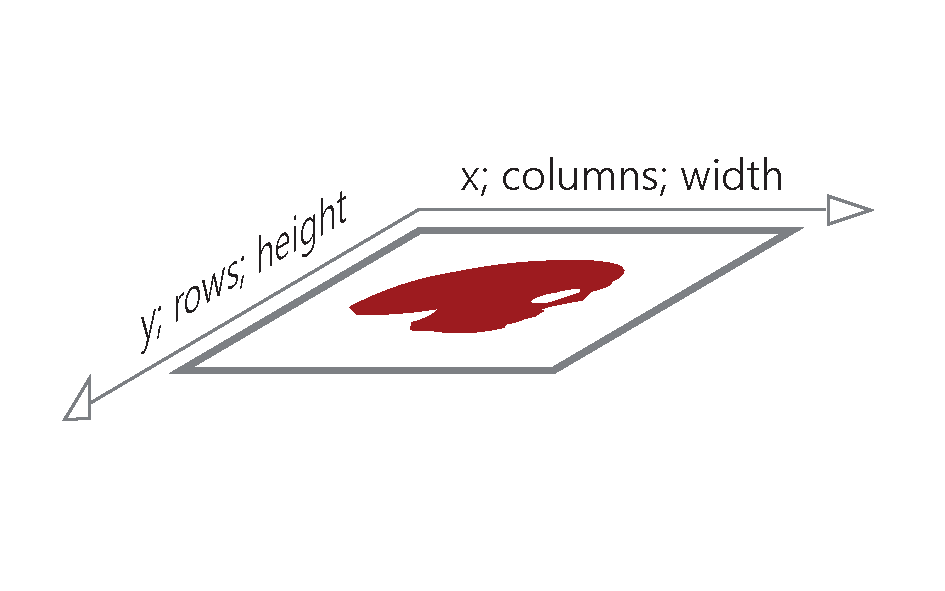
\includegraphics[width=5cm]{./img/2d.pdf} \label{2d}}
\subfigure[3D Bildfolge]{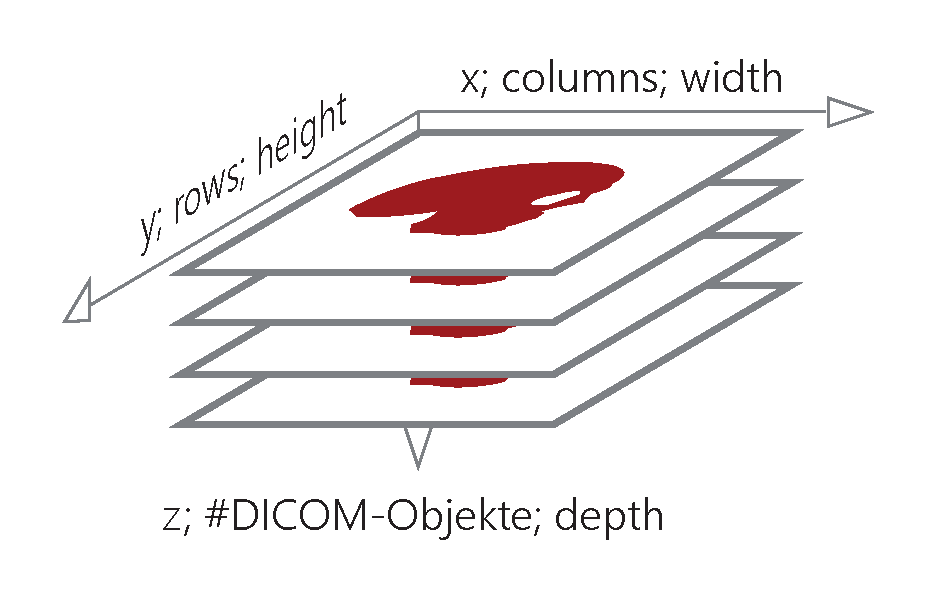
\includegraphics[width=5cm]{./img/3d.pdf} \label{3d}}
\subfigure[zeitlich Abhängige 3D Bildfolge]{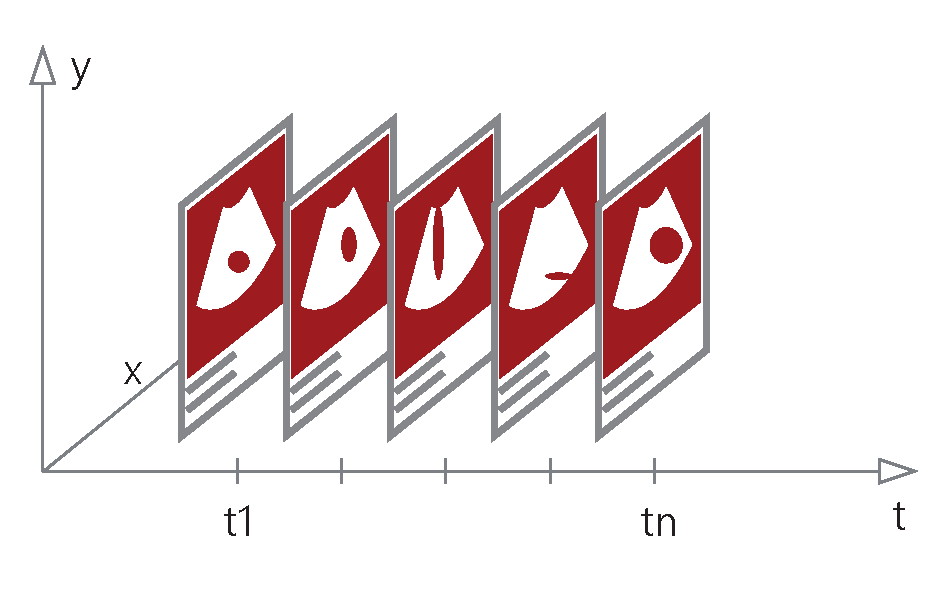
\includegraphics[width=5cm]{./img/time.pdf} \label{time3d}}
}
%\floatfoot{Vorlage für die Grafik der Fensterungstechnik ist\cite[Abbildung 8.1]{handels:mbv}; Die Beispieldaten stammen von http://www.osirix-viewer.com/datasets/ - abgerufen am 19.01.2014}
\caption{Darstellung von 2- und 3-dimensionalen Bilddaten}
\label{dimensions}
\end{figure*}

\section{Bilder mit zeitlicher Abhängigkeit}

Auch Bildaufnahmen zu verschiedenen Zeitpunkten sind dreidimensionale Bildfolgen, wobei die Zeit die dritte Dimension darstellt\cite[2.2.5]{handels:mbv}. Häufige Einsatzgebiete für Bewegtbildfolgen ist die Endoskopie oder Sonographie. Die Abbildung \ref{time3d} macht den Unterschied zwischen zeitlicher und räumlicher Dimension deutlich. Räumliche Darstellungen sind grundsätzlich in mehrere DICOM-Objekte und Dateien aufgeteilt. Zeitlich abhängige Daten sind in einem einzigen Objekt zusammengefasst. NumberOfFrames (0028,0008) gibt die Anzahl an unterschiedlichen Aufnahmen und Zeitpunkten an, die in PixelData enthalten sind.

\part[Entwicklung des Java Medical Imaging Toolkit]{Entwicklung des \\ Java Medical Imaging Toolkit - \\ jMediKit}

\chapter{Softwarearchitektur des Java Medical Imaging Toolkit} \label{architecture}

\section{Die Eclipse Rich Client Platform}

Die Grundlage für eine modulare Entwicklung der Software liefert die Eclipse Rich Client\footnote{Es lässt sich zwischen Rich Clients und Thin Clients unterscheiden. Rich Clients stellen sowohl die Präsentationsschicht als auch die logische Schicht auf dem Client zur Verfügung. Die Applikationsfunktionalität der Thin Clients wird komplett von einem Server bereitgestellt. Die Bedienung erfolgt meist über den Browser.} Platform (RCP). Eclipse, basierend auf der Programmiersprache Java, wird seit 2001 von einer OpenSource-Gemeinde entwickelt\cite{vogel:eclipseoverview}. Während es anfangs rein für die Java-Applikationsentwicklung entworfen wurde, ist es heute eine allgemeine erweiterbare Entwicklungsumgebung. So lässt sich zum einen das Grundprogramm mit Hilfe sogenannter Plug-ins erweitern und zum anderen eigenständige Applikationen erstellen (RCP), die auf dem Eclipse-Framework aufbauen. Das \glqq Aptana Studio\footnote{http://www.aptana.com/}\grqq\ ist beispielsweise ein Plug-in, das der Grundentwicklungsumgebung mehrere Funktionalitäten im Bereich der Webentwicklung (Kommunikation zum Server, Syntaxhighlighting von HTML und CSS) hinzufügt. RSS Owl\footnote{http://www.rssowl.org/}, ein Programm zur Verwaltung von Newsfeeds, ist ein Beispiel für eine eigenständige Rich Client Applikation auf Basis von Eclipse.\\
Eine Kernkomponente des Eclipse-Frameworks ist \textit{Equinox}, eine Implementierung der OSGi-Spezifikation. OSGi bietet die Möglichkeit, modulare Java-Applikationen zu entwickeln und Softwarepakete (nach der Spezifikation \glqq Bundles\grqq\, unter Eclipse \glqq Plug-ins\grqq\ genannt) während der Laufzeit hinzuzufügen, zu entfernen, zu starten oder zu stoppen \cite{vogel:e4overview}. Das Java Medical Imaging Toolkit ist eine Implementierung eines Bundles beziehungsweise Plug-ins.\\
Abbildung \ref{eclipsee4arch} zeigt die Architektur der Eclipse Rich Client Platform.

\begin{figure}[htbp]
  \vspace{0.5cm}
  \centering
  \fbox{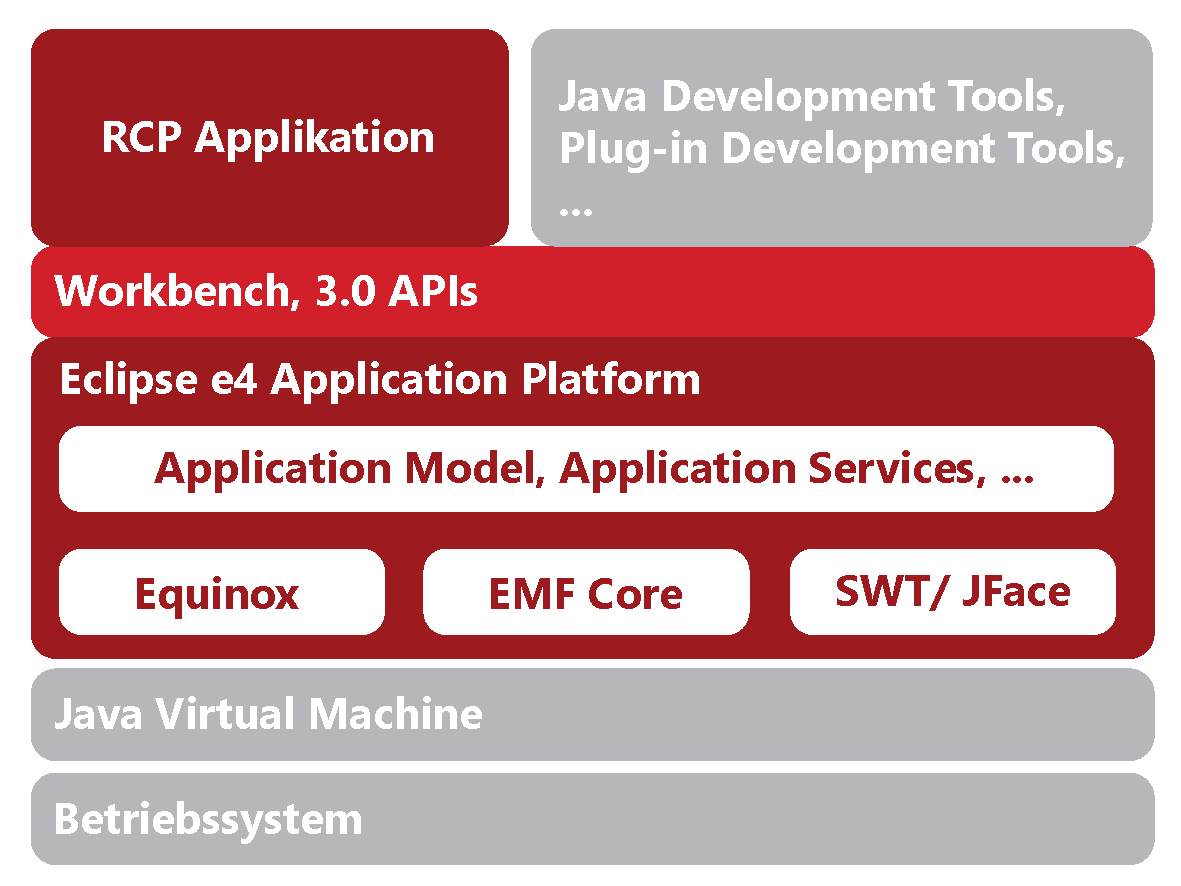
\includegraphics[angle=0,width=10cm]{./img/e4arch.pdf}}
  \caption{Architektur der Eclipse e4 Plattform zur Entwicklung von Rich Client Applikationen}
  \floatfoot{https://wiki.eclipse.org/Eclipse4}
  \label{eclipsee4arch}
  \vspace{0.5cm}
\end{figure}

Die untere Ebene bildet das Betriebssystem. Eclipse kann grundsätzlich plattformunabängig unter Windows, verschiedener Linux Distributionen oder Mac OS eingesetzt werden. Einzige Voraussetzung ist eine installierte Java Virtual Machine. Aufbauend auf Java steht der Eclipse-Kern, bestehend aus dem OSGi-Framework Equinox, dem Eclipse Modeling Framework EMF\footnote{Das EMF dient beispielsweise zur Entwicklung eines Datenmodells, wird allerdings für weitere Ausführungen nicht explizit benötigt.} und dem Standard Widget Toolkit SWT. Das SWT ist eine OpenSource Implementierung verschiedenster grafischer Bedienelemente wie Schaltflächen, Textfelder, Tabellen und vieles mehr.Der Unterschied zu den in Java integrierten grafischen Oberflächen besteht darin, dass das Standard Widget Toolkit auf die Ressourcen des Betriebssystems zugreift und sich in der Darstellung den Betriebssystemstandards anpasst\cite{eclipse:swt}. Aufbauend auf den Grundkomponenten liegt das \textit{Application Model}, das die Struktur der Applikation(Menüs, Fenster, etc.) beschreibt \cite[Kapitel 7]{vogel:e4overview}.\\
Workbench und Eclipse 3.0 APIs bieten noch die Möglichkeit Anwendungen abwärtskompatibel zu entwickeln. Die gesamte Plattform bildet die Basis für das Java Medical Imaging Toolkit. Durch das Application Model kann modular entwickelt und die Programmstruktur in zukünftigen Versionen erweitert werden.

\section{Das Eclipse Application Model}

Damit eine Anwendung strukturiert werden kann stellt das Application Model steuernde und visuelle Elemente zur Verfügung.
\begin{itemize}

\item \textbf{Strukturen zur visuellen Beschreibung der Applikation}\\
	Das Aussehen wird mit Hilfe von Windows, Parts, PartStacks und Anderen beschrieben. Die Elemente enthalten noch keine Logik sondern definieren nur die Struktur der Anwendung.


\item \textbf{Strukturen zur Steuerung des Verhaltens}\\
	 Zu den Komponenten, die das Verhalten der Applikation beeinflussen zählen zum Beispiel Tastatur-Shortcuts, Commands und Handler. Letztere dienen zur Verarbeitung von Benutzereingaben.

\end{itemize}

\subsection{Visuelle Komponenten}

\subsubsection{Window}
Windows sind einfache Repräsentationen eines Fensters der Benutzeroberfläche\cite[org.eclipse.e4.ui.model.application.ui.basic]{eclipse:help}. Sie bilden das Grundgerüst der Applikation und beinhalten Perspectives, PartStacks und andere Elemente. Ein einfaches Fenster ist in Abbildung \ref{rcp_window} zu sehen.

\subsubsection{Menüs}
Ein Menü ist der Container für verschiedene Menü-Elemente und dient dazu Benutzereingaben entgegenzunehmen. Einem Element können Commands hinterlegt werden, damit die Eingaben weiter verarbeitet werden können. Ein Menüpunkt kann selbst ein Menü beinhalten.

\subsubsection{Perspective}
Perspectives beinhalten eine Menge von Elementen der Benutzeroberfläche wie PartStacks und Parts. Perspectives können unabhängig vom Rest der Oberfläche gewechselt werden\cite[org.eclipse.e4.ui.model.application.ui.advanced]{eclipse:help}. So können Perspectives beispielsweise die Anordnung der Parts definieren, oder neue Parts anzeigen, die in einer anderen Perspective nicht zu enthalten sein sollen. Unter Eclipse hat zum Beispiel der Debug-Modul eine eigene Perspective und es kann dynamisch zwischen Debug- und Entwicklungsperspektive gewechselt werden.

\subsubsection{PartSashContainer}
Wie der Name bereits andeutet, ist ein PartSashContainer ein Container für PartStacks und Parts. Die enthaltenen Elemente werden komplett angezeigt. In Abbildung \ref{rcp_partsash} ist eine solche Kombination zu sehen. Die obere Hälfte stellt einen PartStack mit den beiden Parts \textit{TestPart A} und \textit{TestPart B} dar. Der Untere Teil ist ein Stack-unabhängiger Part.

\subsubsection{PartStack}
Auch der PartStack dient als Behälter für einzelne Parts. Der Unterschied zum PartSashContainer liegt darin, dass bei PartStacks nur der aktuell ausgewählte Part angezeigt wird. Die Darstellung des Stacks ist mit üblichen Tabs zu vergleichen, wie Abbildung \ref{rcp_partStack} zeigt. Der Stack enthält die beiden Parts \textit{TestPart A} und \textit{TestPart B}.

\subsubsection{Part}
Ein Part ist die kleinste Einheit des Application Models und ist Kern der Benutzeroberfläche\cite[org.eclipse.e4.ui.model.application.ui.basic]{eclipse:help}. Innerhalb der Parts werden alle weiteren Bedienelemente angezeigt. Jede Abbildung von \ref{rcp_part} - \ref{rcp_partsash} enthält eine oder mehrere Parts. Betrachtet man das Application Model als Baumstruktur, symbolisieren Parts die Blattknoten. Parts können direkt einem Window unterstellt oder tief verschachtelt zwischen Perspectives und Stacks benutzt werden.


\subsection{Steuernde Komponenten}
\subsubsection{Commands}
Commands bilden die abstrakte Schicht zwischen Benutzereingabe und Verarbeitung. Commands besitzen keine eigenen Implementierung. Das ermöglicht dem Entwickler das Verhalten indiviuell zu gestalten. So könnte ein Einfügen-Befehl im Editor ein anderes Verhalten auslösen als im Explorer-Part\cite[org.eclipse.ui.commands]{eclipse:help}.

\subsubsection{Handler}
Handler sind die konkreten Implementierungen der Commands und sind für die Verarbeitung der Benutzereingaben verantwortlich.

\begin{figure*}
%\subfigure[Keypoints]{\includegraphics[width=0.49\textwidth]{./img/basmati_keypoints.png}}\hfill
%\centering

\subfigure[Window]{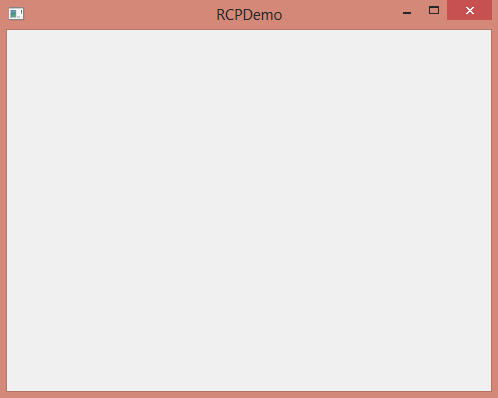
\includegraphics[width=0.40\textwidth]{./img/rcp_window.png} \label{rcp_window}}\hfill
\subfigure[Part]{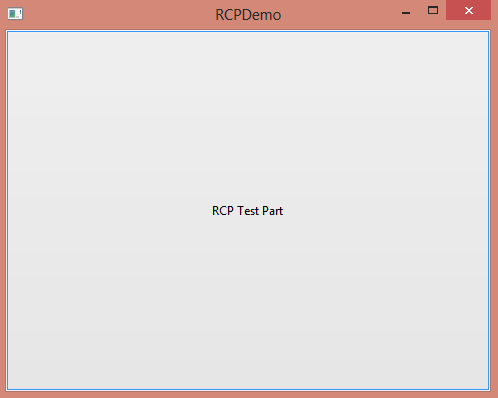
\includegraphics[width=0.40\textwidth]{./img/rcp_part.png} \label{rcp_part}}\\
\subfigure[PartStack]{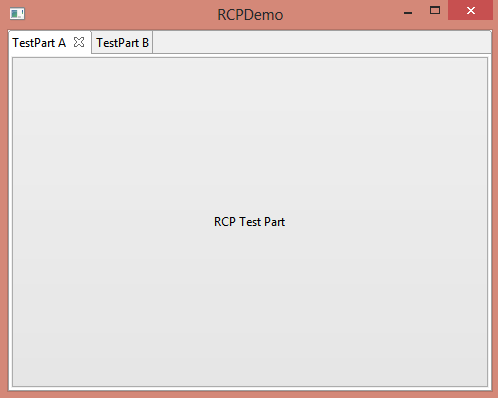
\includegraphics[width=0.40\textwidth]{./img/rcp_partStack.png} \label{rcp_partStack}}\hfill
\subfigure[PartSashContainer]{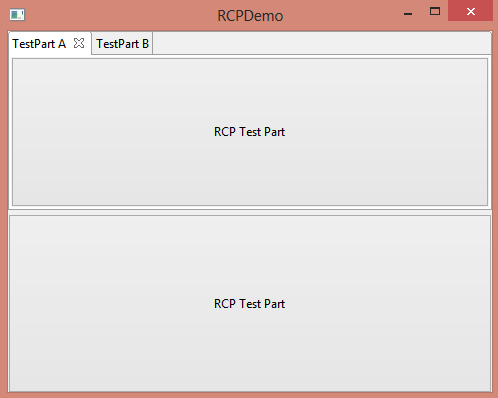
\includegraphics[width=0.40\textwidth]{./img/rcp_partsash.png} \label{rcp_partsash}}

\caption{Verschiedene Elemente des Application Models}
\label{rcp_example}
\end{figure*}

\section{Die Benutzeroberfläche von jMediKit} \label{jmedikit_structure}

Die Oberfläche des Java Medical Imaging Toolkit besteht aus sechs zentralen Elementen.
\begin{enumerate}
\item \textbf{Hauptmenü} \\
	  Das Hauptmenü stellt globale und bildspezifische Operationen zur Verfügung. So werden unter dem Menüpunkt \textit{Erweiterungen} die importierten Plug-ins aufgelistet.
\item \textbf{Werkzeugleiste} \\
	  Dieser Teil der Benutzeroberfläche stellt hauptsächlich Möglichkeiten zur Manipulation der Bilddaten zur Verfügung. Das Kapitel \glqq \ref{implementation}. \nameref{implementation}\grqq\ geht genau auf die verfügbaren Werkzeuge ein.
\item \textbf{DicomBrowser} \\
	  Dieser Part erlaubt die Navigation durch die vom Programm geladenen DICOM-Objekte. Die Anordnung entspricht der Darstellung des ER-Modells aus Kapitel \glqq \ref{grundlagen}. \nameref{grundlagen}\grqq\
\item \textbf{ImageView} \\
	 ImageView übernimmt die Anzeige der Pixeldaten der DICOM-Objekte.
\item \textbf{Console} \\
	Die Konsole dient für die Fehlerausgabe bei der Plug-in-Entwicklung.
\item \textbf{DicomTagView} \\
	Im DicomTagView werden die Tags eines ausgewählten DICOM-Objekts dargestellt.
\end{enumerate}

\begin{figure}[htbp]
  \vspace{0.5cm}
  \centering
  \fbox{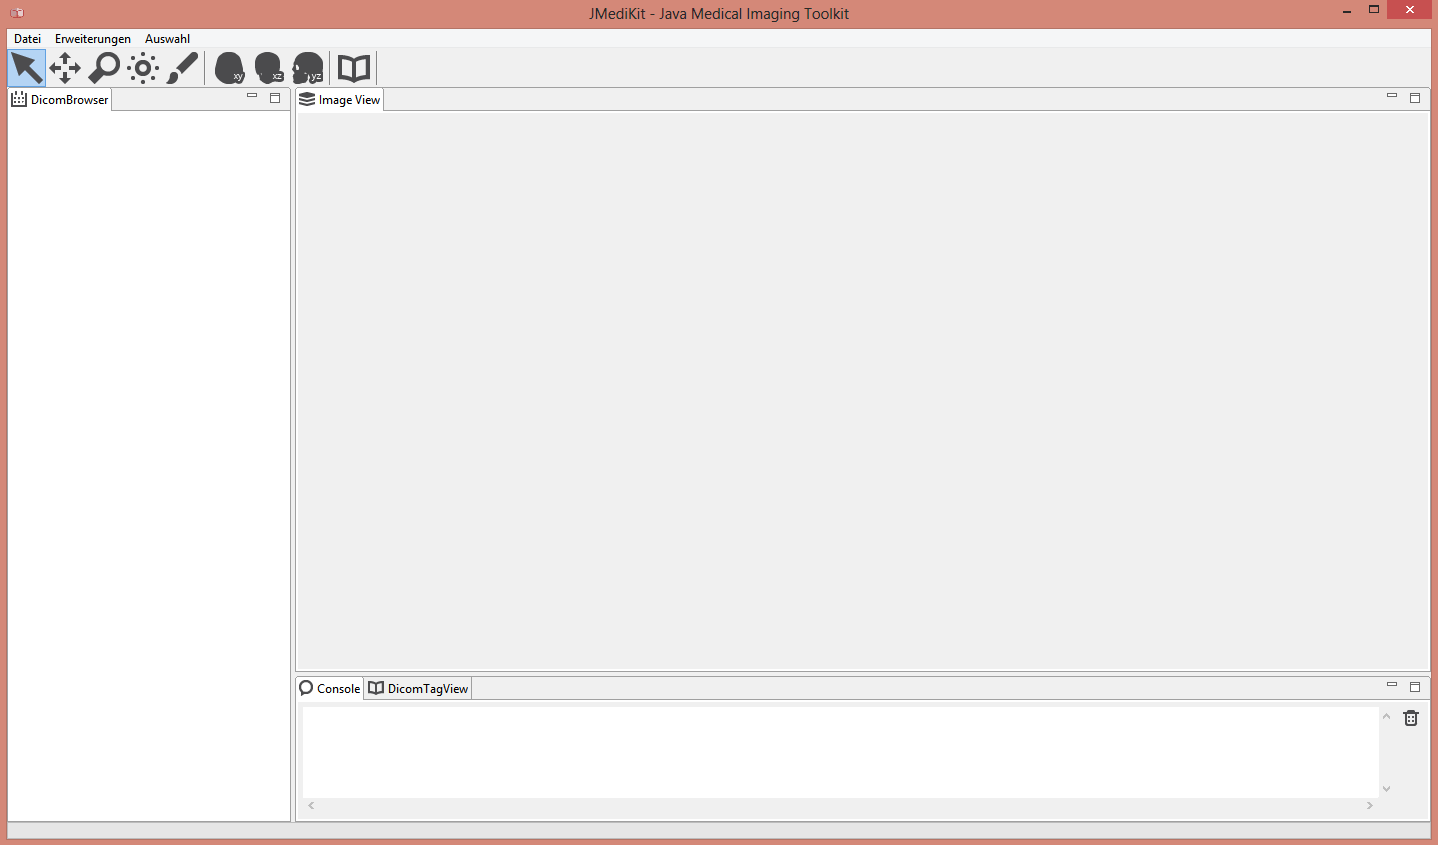
\includegraphics[angle=0,width=12cm]{./img/jmedikit_ui.png}}
  \caption{Die Benutzeroberfläche von jMediKit}
  %\floatfoot{https://wiki.eclipse.org/Eclipse4}
  \label{jmedikitui}
  \vspace{0.5cm}
\end{figure}

Die hierarchische Struktur der Anwendung wird in Abbildung \ref{hierarchy} dargestellt. Die sechs Blattknoten repräsentieren die nach außen für den Benutzer sichtbaren Teil der Anwendung. 


\section{Erweiterbarkeit der Grundstruktur} \label{hierarchyextending}
Die flexible Struktur des Eclipse Application Models und der Rich Client Platform erlauben komfortable Erweiterungen. So können einzelne Parts den schon bestehenden Elementen zugeordnet, oder neue Perspectives eingefügt werden, die eine neue Benutzeroberfläche abbilden könnten. Beispielsweise kann ein neuer Part den FileStack(Abbildung \ref{hierarchy}) damit erweitern, dass DICOM-Objekte von einem PACS geladen werden. Das Kapitel \glqq \ref{extending}. \nameref{extending}\grqq\ zeigt eine Möglichkeit, jMediKit einen neuen Part hinzuzufügen.\\
Durch das Hinzufügen von Elementen des Application Models ist es möglich in die Struktur und vor allem die Benutzeroberfläche einzugreifen. Das bedeutet auch, dass Parts oder andere Strukturen nur in der Lage sind neue Funktionen einzubauen. Es fehlt die Möglichkeit bereits existierende Elemente wie das Hauptmenü (MainMenu) oder die Werkzeugleiste (Toolbar) zu erweitern.
%Damit ist der Teil erfüllt, dass die zu entwickelnde Anwendung für Erweiterungen offen steht. Modulare Werkzeuge %komplettieren die Anforderung der Erweiterbarkeit für Entwickler.

\tikzstyle{every node}=[draw=black,thick,anchor=south, align=center]
%\tikzstyle{selected}=[draw=red,fill=red!30]
\tikzstyle{optional}=[dashed,fill=gray!50]
\begin{figure}[htbp]
\centering
\caption{jMediKit und die hierarchische Anordnung der Elemente des Application Models}
\label{hierarchy}
\begin{tikzpicture}[level distance=1.5cm,
  level 1/.style={sibling distance=3cm},
  level 2/.style={sibling distance=5cm},
  level 4/.style={sibling distance = 6cm, level distance = 2cm},
   level 5/.style={sibling distance=5cm},]
  \node {TrimmedWindow}
  child { node{Mainmenu}}
    child { node{Toolbar}}
    child {node {PerpectiveStack}
      child {node{Perspective}
      	child{node{PartSashContainer}
      	  child{node{PartSashContainer \\ linker Container}
      	    child{node{PartStack \\ FileStack}
      	      child{node{Part \\ DicomBrowser}}
      	    }
      	  }
      	  child{node{PartSashContainer \\ rechter Container}
      	    child{node{PartStack \\ ImageStack}
      	      child{node{Part \\ ImageView}}
      	    }
      	    child{node{PartStack \\ UtilityStack}
      	      child{node{Part \\ Console}}
      	      child{node{Part \\ DicomTagView}}
      	    }
      	  }
      	}
      }
    };
\end{tikzpicture}
\end{figure}

\section{Modulare Werkzeuge}
Ein neuer Eintrag in das Hauptmenü und die Werkzeugleiste ist mit Hilfe der Eclipse RCP-Bordmittel schnell erstellt. Dieser ist allerdings auch unabhängig der bisherigen Menüpunkte. So ist zum Beispiel der Eintrag \textit{Datei öffnen} nicht abhängig vom Menüpunkt \textit{Einstellungen}. Wird ein Eintrag ausgewählt, wird dieser ausgeführt und das Programm wartet auf die nächste Eingabe des Benutzers. Schwierigkeiten gibt es bei den Werkzeugen zur Bildmanipulation. Es kann immer nur ein Werkzeug aktiv ausgewählt sein. Zur Übersetzungszeit ist unklar, welche Werkzeuge wann erzeugt werden müssen. Daraus folgt, dass die verschiedenen Objekttypen der Werkzeuge erst zur Laufzeit erzeugt werden können, abhängig welches Werkzeug vom Benutzer ausgewählt wird. Wie in Abschnitt \ref{fabrikmethod} beschrieben, kann die Fabrik Methode für Anwendungsfälle dieser Art der Objekterzeugung eingesetzt werden. Bei den Klassen wird das Open-Closed-Prinzip beachtet. Die abstrakte Klasse \textit{ATool} gibt ein Grundwerkzeug vor und bietet eine Schnittstelle zur Erweiterung. \textit{AToolFactory} gibt die Vorgehensweise zur Werkzeugerzeugung vor. Abgeleitete Fabriken klassifizieren die Werkzeugkategorien.

\begin{figure}[htbp]
  \vspace{0.5cm}
  \centering
  \fbox{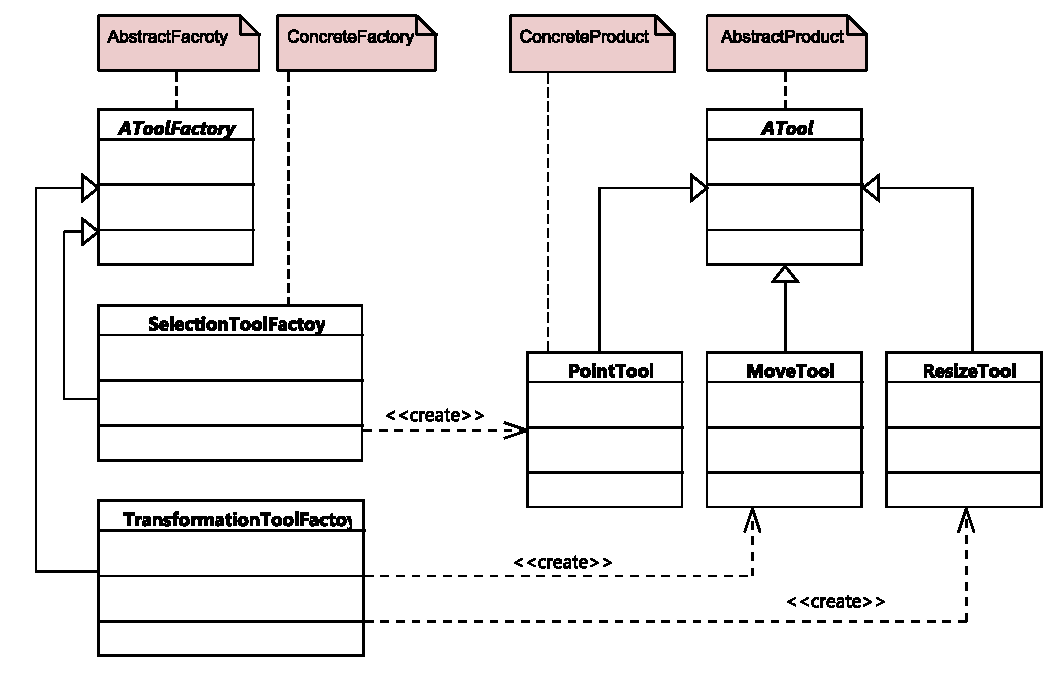
\includegraphics[angle=0,width=12cm]{./img/toolfactory.pdf}}
  \caption{Die Fabrik Methode zur Werkzeugerzeugung}
  %\floatfoot{https://wiki.eclipse.org/Eclipse4}
  \label{toolfactory}
  \vspace{0.5cm}
\end{figure}

Abbildung \ref{toolfactory} zeigt die Umsetzung dieses Erzeugungsmusters. Die Grundversion von jMediKit enthält die zwei konkreten Fabriken \textit{TransformationToolFactory} und \textit{SelectionToolFactory}. Erstere beinhaltet Werkzeuge zur Bildtransformation wie die Skalierung (\textit{ResizeTool}) und letztere enthält ein Werkzeug zur Auswahl von Punkten im Bild(\textit{PointTool}). Sollen weitere Werkzeuge entwickelt werden, können diese von der Superklasse \textit{ATool} abgeleitet werden. Passt das Tool in keine verfügbare Fabrik, kann auch hier eine neue Rubrik erzeugt werden.

\section{Die Plug-in Architektur}

Die Entwicklung von Erweiterungen durch den Anwender spielt eine zentrale Rolle in dieser Abschlussarbeit. Die Entwicklung von zusätzlichen Funktionen und Bedienelemente mittels des Application Models sind erst nach einem erneuten Build-Prozess verfügbar. Es soll den Anwendern eine Möglichkeit geboten werden, eigenständig Erweiterungen zu entwickeln. Der Wirkungsbereich dieser Plug-ins beschränkt sich auf die Manipulation der Bilddaten. Dadurch ist kein explizites Wissen zur Eclipse-Plattform nötig.\\
Die Grundlage der Plug-in Architektur bildet das in Kapitel \ref{swa} vorgestellte Plug-in-Muster. In den Anforderungen ist festgelegt, dass diese Programmerweiterungen sowohl in zwei- als auch dreidimensionaler Richtung arbeiten sollen. Dadurch ist eine Anpassung des Architekturmusters notwendig. Als Ergebnis wird eine Kombination aus Plug-in, Schablonenmethode und Singleton eingesetzt. Das UML-Diagramm in Abbildung \ref{aplugin} zeigt die Architektur und Zusammenarbeit der drei Muster.

%Es ergeben sich verschiedene Probleme bei der Umsetzung Schablone, Singleton, 

\begin{figure}[htbp]
  \vspace{0.5cm}
  \centering
  \fbox{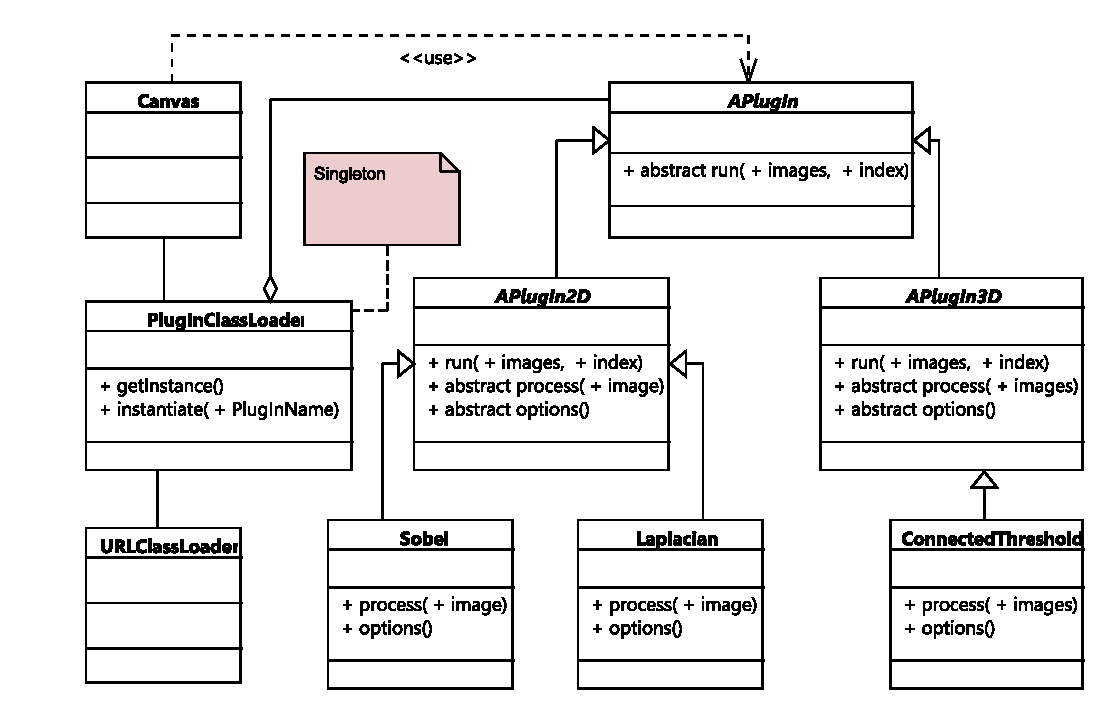
\includegraphics[angle=0,width=12cm]{./img/APlugin.pdf}}
  \caption{Architektur der Plug-in-Struktur}
  %\floatfoot{https://wiki.eclipse.org/Eclipse4}
  \label{aplugin}
  \vspace{0.5cm}
\end{figure}

\subsection{Plug-in als Grundstruktur}
Die Manager-Klasse des Architekturmusters ist \textit{PlugInClassLoader}. Diese Klasse dient sowohl zum Laden der Plug-ins, als auch zum Instantiieren der Plug-in-Objekte. Aufgrund des eingeschränkten Wirkungsbereich der Plug-ins ist die Zeichenfläche der Anwendung(\textit{Canvas}) das einzige Modul, das über den Manager Plug-in-Objekte erzeugen kann.\\
Ein Unterschied zur UML-Darstellung in Abbildung \ref{pluginpattern} besteht darin, dass keine Schnittstelle zur Implementierung, sondern eine abstrakte Klasse \textit{APlugIn} zur Ableitung zur Verfügung gestellt wird. Das bringt den Vorteil, gemeinsame Methoden zu definieren die in allen Plug-ins enthalten sind.
 %jMediKit
%Aufgrund des eingeschränkten Wirkungsbereich der Plug-ins ist die Zeichenfläche der Anwendung das einzige Modul von %jMediKit, das diese Art der Erweiterungen aufrufen ausführen kann. Dadurch besitzt die Manager-Klasse %\textit{PlugInClassLoader} nur eine singuläre Beziehung zur Klasse der Zeichenfläche.

\subsection{Erweiterung mit der Schablonenmethode}
Nach den Anforderungen in Kapitel \ref{anforderungen} ist es nötig, Plug-in-Schnittstellen sowohl für die Entwicklung von zwei- als auch dreidimensionalen Bilddaten anzubieten. Um dies zu erfüllen, stehen dem Benutzer die beiden abstrakten Klassen \textit{APlugIn2D} und \textit{APlugIn3D} zur Verfügung. Beide Varianten repräsentieren die Schablonenmethode. Das Template wird von der Methode \textit{run()} repräsentiert. Der generische Teil des Algorithmus ist \textit{process()}. Die Schablone ist notwendig, da abhängig von 2D und 3D andere Bilddaten an den Benutzer zum Bearbeiten übergeben werden müssen. Nach dem Aufruf von \textit{process()} wird zusätzlich die Rückgabe des Benutzers von der Templatemethode \textit{run()} validiert. Die Schablone ermöglicht dadurch eine Vorverarbeitung und Nachbearbeitung der Bilddaten.
 
\subsection{Singleton als Plug-in Manager}
Der Manager \textit{PlugInClassLoader} ist als Singleton realisiert. Dadurch wird das Problem umgangen, dass mehrere Manager die gleichen Plug-ins laden. Passiert dies, sind gleiche Klassen zueinander inkompatibel und es kann nicht sichergestellt werden, welche Klasse von welchem Manager zur Verfügung gestellt wird.\\
Damit neue Klassen zum Programmstart eingebunden werden können, wird der Java System Classloader über den Manager um einen URL-Classloader erweitert. So werden zu den bisherigen Klassen der Java Virtual Machine alle die Plug-in-Klassen hinzugefügt.

\section{Externe Bibliotheken}

Fremde Bibliotheken werden aus verschiedenen Gründen benötigt. Zum einen für das Lesen von DICOM-Objekten und zum anderen bieten Bildverarbeitungsbibliotheken eine gute Grundlage an Funktionen. Zur Verarbeitung von DICOM-Dateien verwenden jMediKit die freie Bibliothek \glqq dcm4che\grqq. Für die Bildverarbeitung wird \glqq Simple ITK\grqq\ eingesetzt.

\subsection{dcm4che}
Im Kapitel \glqq \nameref{grundlagen}\grqq\ wurden nur die Grundlagen gezeigt. Die Standards zu DICOM-Objekten, Kommunikation und Speicherung sind komplex. Daher wird zur Verarbeitung medizinischer Daten(vor Allem Patienten- und Bilddaten) auf externe Bibliotheken zurückgegriffen. Für eine Implementierung in Java standen folgende zur Auswahl: \textit{Pixelmed}\footnote{http://www.pixelmed.com/} und \textit{dcm4che2}\footnote{http://www.dcm4che.org/}. Beide bieten mit DICOM-Objekt-Verarbeitung und Netzwerkkommunikation ähnliche Dienste.\\
dcm4che.org bietet allerdings eine Software namens \textit{dcm4chee} um ein PACS zu betreiben. Diese wird im Labor für medizische Bildverarbeitung eingesetzt. Das ermöglicht eine leichtere Integration für spätere Erweiterungen von jMediKit in die bestehende Umgebung des Labors.\\
Dcm4che2 wird unter der GNU General Public License. Dies ermöglicht die freie Verwendung der Software. JMediKit setzt die Version 2.028 ein.

\subsubsection{Java Advanced Imaging Image I/O Tools}
Um alle Bildformate (abhängig von der Transfersyntax der DICOM-Objekte werden Bilddaten komprimiert als JPEG oder JPEG200 gespeichert) lesen zu können, verwendet dmc4che2 die Bildverarbeitungsbibliothek \textit{Java Advanced Imaging Image I/O Tools}. Diese ist \textit{nicht} in dcm4che2 integriert und muss vom Anwender selbst auf dem System installiert werden. Die benötigten Dateien und Pakete können unter \textit{http://download.java.net/media/jai-imageio/builds/release/1.1/ - Stand 31.01.2014} bezogen werden.

\subsection{Simple ITK}
Das \textit{Insight Segmentation and Registration Toolkit(ITK)}\footnote{http://www.itk.org/} ist eine umfangreiche Sammlung an Algorithmen zur Segmentierung und Registrierung. Das ITK ist plattformübergreifend einsetzbar und wurde in C++ implementiert. Zwar sind Java- oder Python-Wrapper\footnote{Wrapper machen es möglich, Bibliotheken fremder Sprachen in aktuellen Sprachen einzubinden und zu benutzen. So wäre es möglich, das ITK, welches in C++ implementiert ist, über Wrapper in Java nutzen zu können} verfügbar, für die aktuelle Version 4 war es zum Zeitpunkt der Erstellung dieser Arbeit allerdings nicht möglich zuverlässig einen ITK-Build für eine Verwendung in Java zu erstellen.\\
Das \textit{Simple ITK}\footnote{http://www.simpleitk.org/} bietet eine kompakte Implementierung des ITK. Insgesamt sind 75\% der Klassen aus dem ITK integriert\cite{sitk:filter}. Für einen Einsatz in einer Java Umgebung, kann das Projekt als Java-Bibliothek bezogen werden. Simple ITK steht unter der Apache 2.0 Lizenz und erlaubt eine uneingeschränkte Nutzung.

\subsection{Der Adapter zur Auflösung von Abhängigkeiten}

Eine Nutzung von externen Bibliotheken bedeutet gleichzeitig, dass Abhängigkeiten zwischen dem zu entwickelndem Programm und den fremden Paketen geschaffen werden. Werden bibliotheksspezifische Objekte im Quelltext erzeugt ist man abhängig von einer kontinuierlichen Weiterentwicklung der eingebundenen Projekte. Bei einem Wechsel der Bibliotheken müssen alle referenzierten Objekte angepasst werden und der Code ist nicht mehr ohne erheblichen Mehraufwand wartbar.\\
Mit Hilfe des Adapters werden bei jMediKit die Abhängigkeiten aufgelöst. In Abbildung \ref{dicomo} wird das Klassendiagramm dargestellt. Wie auch das Plug-in Muster wird auch der Adapter mit Anpassungen eingesetzt. Unter jMediKit wird ein DICOM-Objekt aus zwei unterschiedlichen Teilen repräsentiert. Ein Teil (\textit{IDicomData}) beinhaltet den reinen Datenteil. Das bedeutet alle verfügbaren Tags des DICOM-Objekts sind enthalten. Der zweite Teil (IDicomImageData) besteht aus den reinen Pixeldaten. Diese beiden Schnittstellen bilden den Adapter für die externe Bibliothek \textit{dcm4che2}. Durch die Trennung von Daten und Bilddaten bleibt die Flexibilität bei der Bibliothekswahl erhalten. So kann zum Beispiel Simple ITK nur für das Einlesen der Bilddaten verwendet werden, denn es werden keine Methoden zum Auslesen der Tags geboten. Dadurch wäre eine zweite Bibliothek für den Datenteil notwendig. In der Implementierung des Adapters wird in beiden Teilen \textit{dcm4ch2} eingesetzt, da diese Bibliothek sowohl Daten als auch Bilddaten verarbeiten kann. Die beiden Klassen \textit{DicomImageData} und \textit{DicomData} implementieren die Schnittstellten \textit{IDicomImageData} und \textit{IDicomData}. Keine anderen Klassen greifen auf Objekte und Methoden aus den Bibliotheken zu.\\
Um beide Aspekte zu vereinen, stellen die Schnittstellen \textit{IDicomData} und \textit{IDicomImageData} die neuen zu adaptierenden Funktionen dar, die von \textit{ADicomObject} adaptiert werden. Der konkrete Adapter ist \textit{DicomObject}. Um die Abhängigkeiten aufzulösen und die Flexibilität in der Bibliothekswahl zu wahren wird dieser geschachtelte Adapter eingesetzt.

\begin{figure}[htbp]
  \vspace{0.5cm}
  \centering
  \fbox{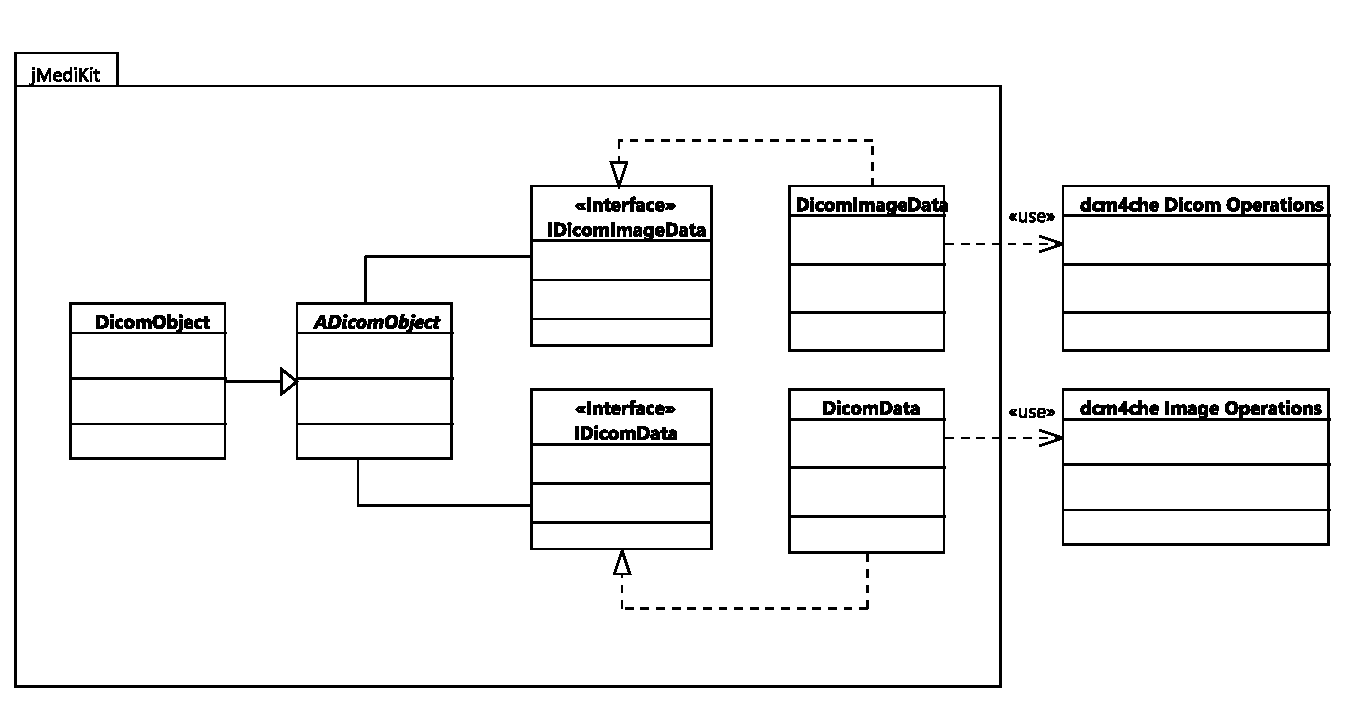
\includegraphics[angle=0,width=12cm]{./img/Dicomo.pdf}}
  \caption{Das Adapter-Muster unter jMediKit}
  %\floatfoot{https://wiki.eclipse.org/Eclipse4}
  \label{dicomo}
  \vspace{0.5cm}
\end{figure}

Zusätzlich wird die Schnittstelle zur Bibliothek vereinfacht, indem nur Funktionen zur Verfügung gestellt werden, die tatsächlich eingesetzt werden. Werden zusätzliche Funktionen benötigt, kann das Interface der Adapter erweitert werden.\\
Soll zukünftig eine Bibliothek getauscht werden, muss nur das Interface neu implementiert werden und die Anwendung kann wie gewohnt eingesetzt werden.

\section{Die Architektur der Bilddaten}

Die Bilddaten sind ein Teil des \textit{ADicomObjects}. Diese werden mit Hilfe der abstrakten Klasse \textit{AImage} dargestellt und enthalten viele zusätzliche Informationen wie Bilddimension, Fensterungsdaten oder die Position des Patienten im Raum. Wie in Kapitel \ref{grundlagen} erläutert, besitzen medizinische Bilder unterschiedliche Grauwert-Tiefen oder Farbdarstellungen. Um die Unterschiedlichen Bildtypen abzubilden stehen die konkreten Klassen \textit{UnsignedByteImage} $\rightarrow$ 8-Bit, \textit{ShortImage} $\rightarrow$ 16-Bit, \textit{UnsignedShortImage} $\rightarrow$ 16-Bit und \textit{IntegerImage} $\rightarrow$ 32-Bit Farbbild zur Verfügung. Ein \textit{ADicomObject} beinhaltet alle Bilddaten der entsprechenden Serie des DICOM-Objekts.\\
Um mit \textit{AImage} zu arbeiten gibt es zwei Möglichkeiten: Die Erste ist das Auslesen über das \textit{ADicomObject}. Hierzu muss ein DICOM-Objekt aus einer Datei eingelesen werden. Im Bereich der Plug-in-Entwicklung ist es sinnvoll leere Bilder zu erzeugen und während der Anwendung des Plug-ins mit neuen Werten zu Füllen. Hierbei hilft die Klasse \textit{SimpleImageFactory}.

\begin{figure}[htbp]
  \vspace{0.5cm}
  \centering
  \fbox{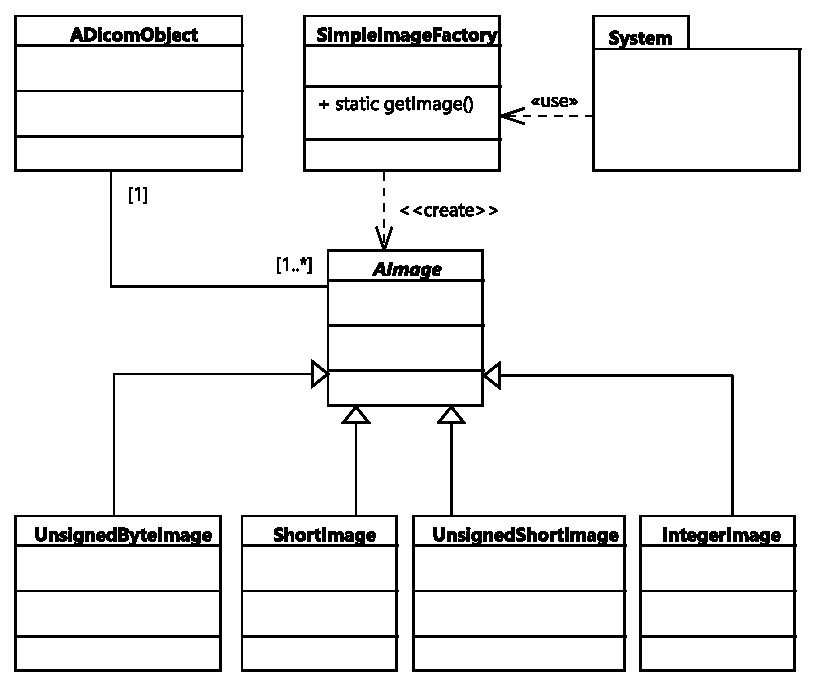
\includegraphics[angle=0,width=12cm]{./img/imagemodel.pdf}}
  \caption{Diagramm zur Klassenstruktur der Bilddaten}
  %\floatfoot{https://wiki.eclipse.org/Eclipse4}
  \label{imagemodel}
  \vspace{0.5cm}
\end{figure}

\subsection{Die einfache Fabrik}

Die einfache Fabrik ist ähnlich der Fabrikmethode, allerdings wird dieses Verfahren der Objekterzeugung nicht den Entwurfsmustern zugeordnet.\\
Beim Entwickeln von Plug-ins können Anwender vor dem Problem stehen, nicht zu wissen, welche Grauwert-Tiefe das aktuell geladene Objekt besitzt. Nur ein mühsames Auslesen über die DICOM-Tags und oder einer Schleife zur Typ-Ermittlung würde Abhilfe schaffen. Der statischen Methode \textit{getImage()} von \textit{SimpleImageFactory} kann der Bildtyp des DICOM-Objekts übergeben werden, worauf ein typgerechtes Bildobjekt erzeugt und zurückgegeben wird.

\subsection{Struktur der Bilder im ImageViewPart}

Da die Struktur der Bilddaten dargestellt wurde, kann nun die Vorgehensweise zur Anzeige dieser vorgestellt werden.\\

\begin{figure}[htbp]
  \vspace{0.5cm}
  \centering
  \fbox{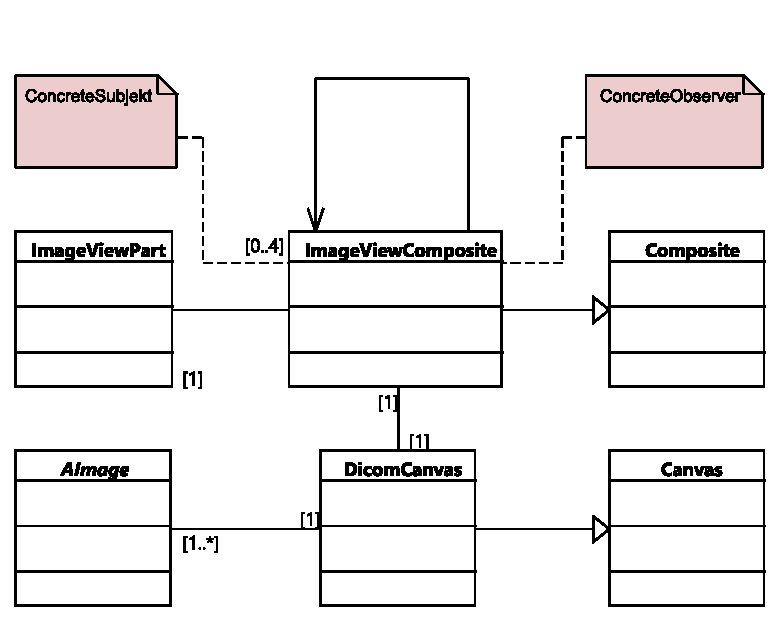
\includegraphics[angle=0,width=12cm]{./img/imageview.pdf}}
  \caption{Organisation der Klassen zur Anzeige der DICOM-Bilddaten}
  %\floatfoot{https://wiki.eclipse.org/Eclipse4}
  \label{imageview}
  \vspace{0.5cm}
\end{figure}

Auf der Benutzeroberfläche findet dieser Vorgang im ImageView Part statt (Abschnitt \ref{hierarchyextending}). Wie in Abbildung \ref{imageview} zu sehen, bildet \textit{ImageViewPart} die Grundlage und dient als Elternelement eines \textit{ImageViewComposites}, von diesen maximal vier zum gleichen Zeitpunkt angezeigt werden können. \textit{ImageViewComposites} erben von der SWT-Klasse \textit{Composite} und enthalten weitere Bedienelemente für den Benutzer. Hierzu zählt die Scrollleiste am rechten Rand wie in Abbildung \ref{iv:1} zu sehen ist. Mit diesem Scrollbalken wird die Schicht aus den dreidimensionalen Bilddaten gewählt, die vom \textit{DicomCanvas} angezeigt werden soll. Die Superklasse von \textit{DicomCanvas} gehört ebenfalls zum Repertoire des SWT und ist das zentrale Element zur Bildanzeige. \textit{DicomCanvas} enthält sämtliche Bilder des DICOM-Objekts.

\begin{figure*}[htb]
%\subfigure[Keypoints]{\includegraphics[width=0.49\textwidth]{./img/basmati_keypoints.png}}\hfill
\centering
\fbox{
\subfigure[Darstellung eines ImageViewComposite]{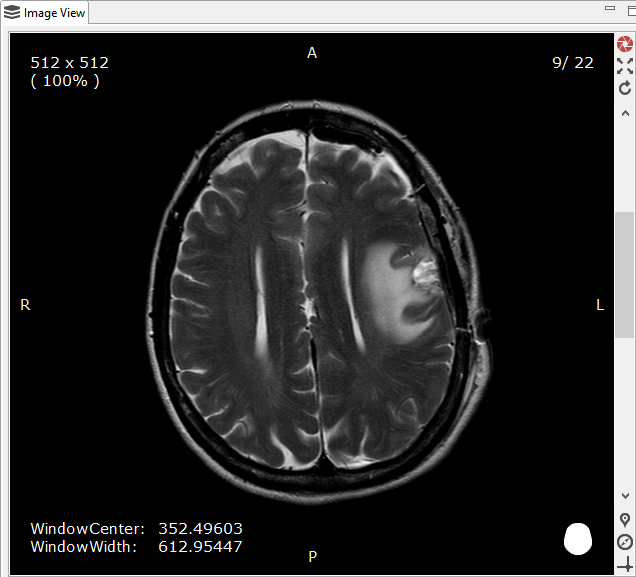
\includegraphics[width=5cm]{./img/ivcomposite.png} \label{iv:1}}
\subfigure[Vier ImageViewComposites im ImageViewPart]{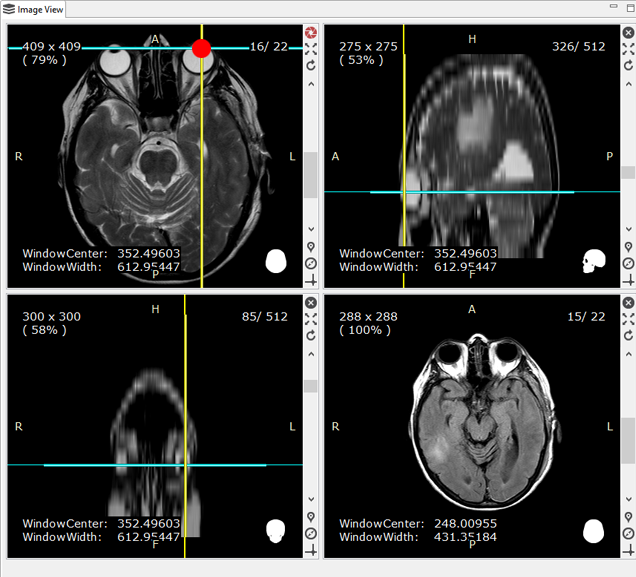
\includegraphics[width=5cm]{./img/ivcomposite4.png} \label{iv:4}}
}
\caption{Benutzeroberfläche der ImageViewComposites}
\label{ivcomposite}
\end{figure*}

Abbildung \ref{iv:4} zeigt vier \textit{ImageViewComposites}, wobei alle außer Composite unten rechts die gleichen DICOM-Objekte anzeigen.
Angenommen ein Benutzer führt einen Klick mit der rechten Maustaste auf den in rot markierten Punkt aus, müssen alle \textit{ImageViewComposites} den gleichen Punkt im dreidimensionalen Raum referenzieren. Dieser wird durch den Schnittpunkt der Linien angezeigt. Eine genaue Beschreibung dazu befindet sich in Kapitel \ref{implementation}.\\
Damit dieses Verhalten von Seiten der Architektur unterstützt wird, muss sichergestellt werden, dass die \textit{ImageViewComposites} untereinander kommunizieren können, dass eine Änderung stattgefunden hat.\\
Aus dem Kapitel \ref{swa} löst das Observer-Muster diese Anforderungen. Der Zyklus in Abbildung \ref{imageview} zeigt die Funktionsweise. Jede ImageViewComposite ist gleichzeitig \textit{ConcreteSubject} als auch \textit{ConcreteObserver}. Das bedeutet, bei jeder Registrierung eines neuen DICOM-Objekts wird geprüft, ob dieses schon im \textit{ImageViewPart} vorhanden ist. Ist dies der Fall, wird es als neuer Observer an bisherigen Subjects angemeldet.\\
Bei diesem Einsatz besteht die Gefahr einer Endlosschleife, wenn der Zyklus nicht beachtet wird. Die Schleife tritt ein wenn ein Subject die Observer benachrichtigt, die Observer ändern den Status und benachrichtigen darauf wiederum ihre Beobachter und so weiter. Bei der Implementierung von jMediKit wird eine Änderung angenommen und das \textit{DicomCanvas} neu gezeichnet und löst keine Rückmeldung einer Änderung aus. \\
Auf dieser Architekturgrundlage findet die im folgenden Kapitel erläuterte Implementierung statt.

\chapter{Implementierung} \label{implementation}

\section{Module}


\chapter{Entwicklung von Erweiterungen} \label{extending}

Das Java Medical Imaging Toolkit bietet sowohl dem Enwickler, als auch dem Anwender Spielraum, die Anwendung zu erweitern. Dieses Kapitel beschreibt die Entwicklung verschiedener Plug-ins in zwei- und dreidimensionalem Raum. Zusätzlich zeigt der Entwurf eines neuen Moduls und eine Implementierung eines Werkzeugs wie die Basisfunktionen von jMediKit erweitert werden.

\section{Entwicklung von Plug-ins}

Die Entwicklung von Plug-ins ermöglicht eine Funktionserweiterung der Anwendung, ohne einen neuen Buildprozess. Bei Programmstart wird der in der Anwendung angegebene Plug-in-Ordner nach allen verfügbaren Erweiterungen durchsucht und eingebunden. Damit Plug-ins vom Programm korrekt gefunden werden können, müssen diverse Konventionen bei der Entwicklung beachtet werden, die im nächsten Abschnitt erläutet werden.

\subsection{Konventionen}
Damit der Importvorgang der Plug-ins ohne Komplikationen verläuft, ist die Anwendung auf die Konsistenz der Plug-ins angwiesen. Die folgenden Konventionen bestimmen diese Konsistenz.

\begin{itemize}
\item \textbf{Generalisierung}\\
Die Basisklasse eines Plug-ins ist entweder \textit{APlugIn2D} oder \textit{APlugIn3D} und muss diese erweitern. 
\item \textbf{Klassenname}\\
Der Name der Klasse des Plug-ins, die von \textit{APlugIn2D} oder \textit{APlugIn3D} erbt, muss mit \textit{zwei Unterstrichen} beginnen. Zusätzlich muss das erste Zeichen ein Buchstabe oder eine Ziffer sein. Listing \ref{regexp} zeigt den regulären Ausdruck zur Beurteilung gültiger Namen. Korrekt sind zum Beispiel \textit{\_\_Test} oder \textit{\_\_3DTest\_Plug\_in}. Ungültig ist beispielsweise \textit{\_Test} oder \textit{\_\_\_TestPlugIn}.
Da ein Plug-in in Beziehung zu anderen Klassen oder Paketen stehen kann, die entweder selbst implementiert oder von Bibliotheken zur Verfügung gestellt werden, wird so die Hauptklasse der Erweiterung kenntlich gemacht.
\item \textbf{Ordnername}\\
Der Ordner, in dem ein Plug-in enthalten ist, muss den identischen Namen wie die Hauptklasse des Plug-ins haben. Ist dieser Name \textit{\_\_Test}, muss der \textit{Wurzelordner} der die Erweiterung enthält ebenfalls \textit{\_\_Test heißen}.
\item \textbf{Ordnerstruktur}\\
Wenn Plug-ins mit Hilfe der Eclipse-Entwicklungsumgebung entwickelt werden, entspricht der bin-Ordner der korrekten Struktur. Ist die Hauptklasse nicht in einem Package organisiert, liegt die Plug-in-Klasse direkt im Plug-in-Ordner und hätte die Struktur \textit{/plugins/\_\_Test/\_\_Test.class}. Erfolgt die Entwicklung mit Packages ist die Struktur \textit{/plugins/\_\_Test/de/korb/\_\_Test.class} wenn die Klasse \_\_Test im Package \textit{de.korb} liegt. \textit{/plugins} ist der Ordner, der die einzelnen Plug-ins enthält. Dieser muss in den Einstellungen der Anwendung spezifiziert werden. Das bedeutet, dass jMediKit alle Plug-ins in \textit{/plugins} findet, wenn die Ordner mit doppeltem Unterstrich beginnen und eine \textit{.class}-Datei mit identischen Namen beinhalten, die APlugIn2D oder APlugIn3D generalisieren. Abbildung \ref{filesystemplugin} zeigt die Ordnerstruktur zweier Plug-ins. \_\_PlugInA ist ohne, während \_\_PlugInB mit Packages organisiert wird. \_\_PlugInB definiert zusätzlich eine eigenen Bibliotheksklasse. Wird der Ordner \textit{plugins} in den Einstellungen angegeben, werden bei Programmstart die beiden Plug-ins initialisiert und können verwendet werden.
\end{itemize}

\lstset{
language=sh,
caption={Der reguläre Ausdruck gültiger Klassennamen},
label=regexp,
xleftmargin=1em,
xrightmargin=1em,
numbers=left,
backgroundcolor=\color{lgrey},
}  
\begin{figure}[htbp]
\begin{lstlisting}[frame=leftline]
^_[A-Za-z0-9].*
\end{lstlisting}
\end{figure}

\tikzstyle{every node}=[draw=black,thick,anchor=west]
%\tikzstyle{selected}=[draw=red,fill=red!30]
\tikzstyle{optional}=[dashed,fill=gray!50]
\begin{figure}[htbp]
\centering
\caption{Beispiel der Ordnerstruktur zwei verschiedener Plug-ins}
\label{filesystemplugin}
\begin{tikzpicture}[%
 grow via three points={one child at (0.5,-0.7) and
  two children at (0.5,-0.7) and (0.5,-1.4)},
  edge from parent path={(\tikzparentnode.south) |- (\tikzchildnode.west)}]
  \node {plugins}
    child[missing]{}
    child{ node{\_\_PlugInA}
      child[missing]{}
      child { node{\_\_PlugInA.class}}
    }
    child[missing]{}
    child[missing]{}
    child[missing]{}
    child { node{\_\_PlugInB}
      child[missing]{}
      child { node{de}
        child{ node{core}
          child{node{\_\_PlugInB.class}} 
        }
        child[missing]{}
        child{ node{lib}
          child{node{Library.class}} 
        }
      }
    };		
\end{tikzpicture}
\end{figure}


    	%child { node{\_\_PlugInA.class}}
    	
    	%child { node{\_\_PlugInB}
    	   %child { node{de}
    	   %  child{ node{core}
    	   %    child{node{\_\_PlugInB.class}} 
    	   %  }
    	   %  child{ node{lib}
    	   %    child{node{Library.class}} 
    	   %  }
    	   %}
    	%}
\FloatBarrier
\subsection{Die Klassenstruktur eines Plug-ins}

Das Java Medical Imaging Toolkit stellt zwei Typen von Plug-ins bereit. Der Anwender kann mit einer Erweiterung von APlugIn2D entweder im zweidimensionalen oder mit APlugIn3D im dreidimensionalen Raum arbeiten. Unabhängig vom Plug-in-Typ müssen zwei abstrakte Methoden der jeweiligen Basisklasse implementiert werden.

\begin{itemize}
\item \textbf{options}\\
Die Methode \textit{options} wird \textit{einmalig} \textit{vor} der Ausführung des Plug-ins aufgerufen. Hier können wahlweise Parameter gesetzt werden, die für weitere Berechnung benötigt werden.
\item \textbf{process}\\
Das Kernelement eines Plug-ins stellt \textit{process} dar. Als Parameter ist entweder das aktuell gewählte Bild im ImageView oder im Fall eines 3D-Plug-ins der Bildstapel übergeben. Beim Rückgabewert muss beachtet werden, dass die Bildanzahl mit der im Parameter übereinstimmt, da sonst weitere Berechnungen wie zum Beispiel die Ebenenrekonstruktionen nicht korrekt ausgeführt werden können.

\end{itemize}

In Listing \ref{zweid} ist die Basisdefinition eines zweidimensionalen Plug-ins dargestellt. Es werden die abstrakten Methoden \textit{process} und \textit{options} implementiert. Mit dem Parameter \textit{img} in \textit{process} können die Pixelwerte manipuliert werden. Das Rückgabebild wird anschließend im ImageView an Stelle des entsprechenden Index angezeigt.

\lstset{
language=Java,
caption={Definition des konkreten 2D-Plug-ins \_\_2dPlugIn.java},
label=zweid,
xleftmargin=1em,
xrightmargin=1em,
numbers=left,
backgroundcolor=\color{lgrey},
}  
\begin{figure}[htbp]
\begin{lstlisting}[frame=leftline]
public class __2dPlugIn extends APlugIn2D{
 @Override
 public AImage process(AImage img){
   return img;
 }
 
 @Override
 public int options(){
   return 0;
 }
}
\end{lstlisting}
\end{figure}

Ein dreidimensionales Plug-in erbt die gleiche Grundstruktur wie das 2D-Plug-in. Wie in Listing \ref{dreid} zu sehen ist, unterscheiden sich die übergebenen Parameter in der Methode \textit{process}. Eine 3D-Erweiterung erhält den gesamten Bildstapel als Liste. Die Variable \textit{index} enthält den Index der Bildschicht, die im  aktiven ImageView angezeigt wird.

\lstset{
language=Java,
caption={Definition des konkreten 3D-Plug-ins \_\_3dPlugIn.java},
label=dreid,
xleftmargin=1em,
xrightmargin=1em,
numbers=left,
backgroundcolor=\color{lgrey},
}  
\begin{figure}[htbp]
\begin{lstlisting}[frame=leftline]
public class __3dPlugIn extends APlugIn2D{
 @Override
 public AImage process(List<AImage> images, int index){
   return images;
 }
 
 @Override
 public int options(){
   return 0;
 }
}
\end{lstlisting}
\end{figure}



\FloatBarrier
\subsection{Nützliche Funktionen}

Neben den Bilddaten stellt jMediKit weitere Funktionen für die Plug-in-Entwicklung zur Verfügung. So können DICOM-Objekte und ganze Bäume zusätzlich geladen werden und Tags und Bilder aus den Objekten zur Verarbeitung gelesen werden. Die dynamische Parameterübergabe stellt eine weitere Funktion dar, die es ermöglicht, eigenen Optionsdialoge für Plug-ins zu erstellen. In folgender Liste werden diese Features genauer erläutert.

\subsubsection{Erstellung eines Bildes vom Typ AImage}
Bilder können unter jMediKit auf zwei Arten erzeugt werden. Mit expliziter Bilderzeugung kann das Objekt entsprechend dem gewünschten Bildtyp direkt instantiiert werden.\\
In vielen Fällen ist der Typ des Parameterbildes in \textit{process} unbekannt und der Anwender ist von einer impliziter Objekterzeugung abhängig. Mit der statischen Methode \textit{getAbstractImage} der Klasse \textit{SimpleImageFactory} kann der Bildtyp eines Referenzbildes übergeben werden. Entsprechend der Referenz wird ein neues Bildobjekt mit passendem Typ zurückgegeben. Listing \ref{ieimg} zeigt jeweils ein Beispiel der Objekterzeugung.

\lstset{
language=Java,
caption={Erzeugung eines AImage},
label=ieimg,
xleftmargin=1em,
xrightmargin=1em,
numbers=left,
backgroundcolor=\color{lgrey},
}  
\begin{figure}[htbp]
\begin{lstlisting}[frame=leftline]
//Explizite Bilderstellung
AImage simg = new ShortImage(800, 600);
System.out.println(simg.getImageType());
//prints 2

//Explizite Bilderstellung
AImage usimg = new UnsignedShortImage(800, 600);
System.out.println(usimg.getImageType());
//prints 3
		
//Implizite Bilderstellung
AImage i_simg = SimpleImageFactory.getAbstractImage(simg.getImageType(), 800, 600);
System.out.println(i_simg.getImageType());
// prints 2
\end{lstlisting}
\end{figure}

\subsubsection{Erzeugung eines SimpleITK-Bildes}

Bildobjekte von jMediKit und SimpleITK sind zueinander inkompatibel. Mit Hilfe von Konvertierungsfunktionen in beide Richtungen wird dieses Problem behoben. Die Anwendung erfolgt ähnlich der \textit{SimpleImageFactory} mit dem Unterschied, dass als Parameter das Bild selbst übergeben wird und eine Kopie als entsprechender Typ und Format zurückgegeben wird. Listing \ref{itkimg} zeigt ein Beispiel einer Konvertierung. Die Klasse \textit{SimpleITKFactory} stellt die Funktionen \textit{getITKImage} und \textit{getAImage} zu einer Konvertierung bereit.

\lstset{
language=Java,
caption={Konvertierung der Bildobjekte zwischen jMediKit und SimpleITK},
label=itkimg,
xleftmargin=1em,
xrightmargin=1em,
numbers=left,
backgroundcolor=\color{lgrey},
}  
\begin{figure}[htbp]
\begin{lstlisting}[frame=leftline]
AImage simg = new ShortImage(800, 600);

Image itk_img = SimpleITKFactory.getITKImage(simg);
String type = itk_img.getPixelIDTypeAsString();
System.out.println(type);
//prints 16-bit signed integer
		
AImage converted_img = SimpleITKFactory.getAImage(itk_img);
System.out.println(converted_img.getImageType());
//prints 2
\end{lstlisting}
\end{figure}

\subsubsection{Saatpunkte und ROIs auslesen}

Die Anwendung stellt die zwei Selektionswerkzeuge \textit{PointTool} und \textit{ROITool} bereit. Zum einen können Punkte gesetzt und zum anderen Bildbereiche markiert werden. Jede Bildinstanz stellt, wie in Listing \ref{select} zu sehen, jeweils einen Getter bereit, der eine Liste der Datenstruktur zurück gibt.

\lstset{
language=Java,
caption={Saatpunkte und Regions Of Interest aus einem AImage ermitteln},
label=select,
xleftmargin=1em,
xrightmargin=1em,
numbers=left,
backgroundcolor=\color{lgrey},
}  
\begin{figure}[htbp]
\begin{lstlisting}[frame=leftline]
@Override
public AImage process(AImage arg0) {
  //doStuff();

  ArrayList<Point2D<Float>> points = arg0.getPoints();
  ArrayList<ROI> rois = arg0.getROIs();
  
  //doThings();
}
\end{lstlisting}
\end{figure}

\subsubsection{Import eines DICOM-Baums}

Ist es notwendig, dass ein zusätzlicher DICOM-Baum in das Plug-in geladen werden muss, gibt es die Klasse \textit{PlugInDicomImporter} mit der statischen Methode \textit{recursiveImport}. Übergibt man ein Verzeichnis, wird dieses rekursiv auf der Suche nach DICOM-Objekten durchlaufen und ein Baum erstellt, der nach den Objekten durchsucht werden kann. Listing \ref{importer} zeigt einen Import und das Auslesen eines DICOM-Objekts.

\lstset{
language=Java,
caption={Saatpunkte und Regions Of Interest aus einem AImage ermitteln},
label=select,
xleftmargin=1em,
xrightmargin=1em,
numbers=left,
backgroundcolor=\color{lgrey},
}  
\begin{figure}[htbp]
\begin{lstlisting}[frame=leftline]
DicomTreeRepository tree = PlugInDicomImporter.recursiveImport(new File("PathToDirectory"));
DicomObject obj = (DicomObject) tree.lookUpDicomTreeItem("UID");
\end{lstlisting}
\end{figure}

\subsubsection{DICOM-Tags aus DICOM-Objekten auslesen}
Neue DICOM-Objekte können entweder durch das Auslesen eines DICOM-Baums erstellt, oder durch die explizite Instantiierung durch Angabe eines Dateipfads. Zuerst wird das Objekt entsprechend der Zeile $5$ oder Zeile $9$ wie in Listing \ref{readObjs} erzeugt. Die Klasse \textit{DicomObject} stellt unter anderem die Methode \textit{getTagData}(in Zeile $14$) zur Verfügung und erhält als Parameter eine Stringrepräsentation des Tags und den Typ des Rückgabewertes. Alle möglichen Typen sind in \textit{DicomObject} als Konstanten festgelegt und müssen entsprechend der Value Representation des Tags gesetzt werden. \textit{PatientName} hat als VR \textit{PN} und wird als Zeichenkette behandelt. Dadurch wird als Rückgabetyp \textit{DicomObject.RETURN\_STRING} gewählt.

\lstset{
language=Java,
caption={Lesen eines Tags aus einem DICOM-Objekt},
label=readObjs,
xleftmargin=1em,
xrightmargin=1em,
numbers=left,
backgroundcolor=\color{lgrey},
}  
\begin{figure}[htbp]
\begin{lstlisting}[frame=leftline]
File d = new File("PathToDirectory");
File f = new File("PathToFile");
		
DicomTreeRepository r = PlugInDicomImporter.recursiveImport(d);
DicomObject obj = (DicomObject) r.lookUpDicomTreeItem("UID");
		
//oder
try {
  DicomObject obj = new DicomObject(f);
} catch (IOException e) {
  e.printStackTrace();
}
		
String name = (String) obj.getTagData("PatientName", DicomObject.RETURN_STRING);
\end{lstlisting}
\end{figure}

\subsubsection{Erstellung eines Dialogfensters}
In Kapitel \ref{implementation} Abschnitt \ref{dynamicParameter} wurden alle Dialogoptionen für eine dynamische Parametervergabe gezeigt. Listing \ref{dynamicex} zeigt die Anwendung eines \textit{GenericPlugInDialog}.\\
Innerhalb des Plug-ins wird der Dialog \textit{dialog} als Datenelement hinterlegt, damit die Werte von \textit{process} ausgelesen werden können. In der Methode \textit{options} wird der Dialog erzeugt und die Dialogelemente hinzugefügt. Die RadioGroup nimmt als Parameter den Namen\footnote{Der Name dient zur eindeutigen Zuordnung, um später die Werte auslesen zu können.}, ein Array von Strings, welche die einzelnen Elemente der Gruppe symbolisieren und einen Standartwert welches Element ausgewählt dargestellt werden soll.\\
Der Slider bekommt ebenfalls einen Namen und den Standardwert, gefolgt von Anfangswert, Endwert, Schrittweite und Nachkommastellen. Im Beispiel können im Slider Werte von $0.0$ - $3.0$ gewählt werden, also $max(\frac{30}{10^1})$. Eine Inkrementierung der Nachkommastelle erhöht die Genauigkeit. Zwei Nachkommastellen des Intervalls $[0,3]$ erlauben Werte zwischen $0.00$ - $3.00$. Ein Intervall $[0,30]$ mit zwei Nachkommastellen kann mit dem Aufruf \textit{dialog.addSlider(\glqq Name\grqq, 1, 0, 3000, 1, 2)} erzeugt werden($max(\frac{3000}{10^2})$).

\lstset{
language=Java,
caption={Erstellung eines eigenen Optionsdialog},
label=dynamicex,
xleftmargin=1em,
xrightmargin=1em,
numbers=left,
backgroundcolor=\color{lgrey},
}  
\begin{figure}[htbp]
\begin{lstlisting}[frame=leftline]
public class __DialogExample extends APlugIn2D{

  GenericPlugInDialog dialog;
	
  @Override
  public AImage process(AImage arg0) {

    String interpolation = (String) dialog.getItemValue("Interpolation");
    float sigma = (float) dialog.getItemValue("Sigma");
	    
    return arg0;	
  }
 
  @Override
  protected int options() {
		
    dialog = new GenericPlugInDialog("Hallo Dialog", "Ein Beispieldialog");	
    dialog.addRadioGroup("Interpolation", new String[]{"NN", "bilinear", "bicubic"},  1);
    dialog.addSlider("Sigma", 1, 0, 30, 1, 1);
    int status = dialog.open();	
    return 0;
  }
}
\end{lstlisting}
\end{figure}

Die Abbildung \ref{dialog_example} zeigt die visuelle Darstellung des individuellen Dialogs, der in \textit{options} zusammengesetzt wurde. 

\begin{figure}[htbp]
  \vspace{0.5cm}
  \centering
  \fbox{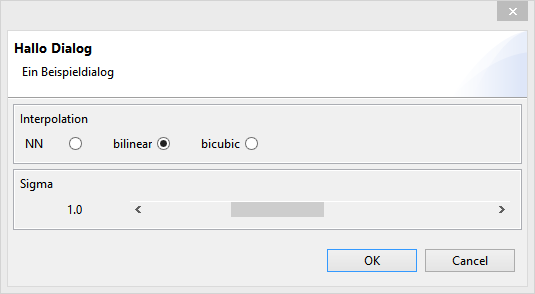
\includegraphics[angle=0,width=8cm]{./img/dialog_example.png}}
   \caption{Die visuelle Darstellung des Dialogs aus Listing \ref{dynamicex}}
  \label{dialog_example}
  \vspace{0.5cm}
\end{figure}

\FloatBarrier
\subsection{Der Laplace Operator}

Der Laplace Operator wird zur Schärfung von Bildern eingesetzt und dient als Beispiel für die Umsetzung eines zweidimensionalen Plug-ins. Die \textit{process}-Methode aus Listing \ref{laplace} zeigt eine Implementierung des Filters. Der Parameter \textit{arg0} enthalt die aktuelle Bildschicht des aktiven ImageViews.\\
In Zeile $6$ wird mit Hilfe der einfachen Fabrikfunktion das Bild für die Filterergebnisse erzeugt, da der Bildtyp von \textit{arg0} nicht explizit bekannt ist. In Zeile $16$ wird das Quellbild \textit{arg0} durchlaufen und gefiltert. In Zeile $31$ wird \textit{copySignificantAttributes} aufgerufen. Damit werden essentielle Bildeigenschaften vom Parameterbild in das aufrufende Bild kopiert. Zu den Eigenschaften zählen zum Beispiel \textit{WindowWidth}, \textit{WindowCenter} oder \textit{ImagePosition}.\\
Sind diese Werte vom Anwender im Rückgabewert von \textit{process} nicht gesetzt, werden die Eigenschaften von \textit{arg0} in das Ergebnisbild kopiert. Damit wird eine korrekte Anzeige im ImageView garantiert.\\
Nach der Rückgabe des geschärften Bildes, wird es von der Anwendung angezeigt.

\lstset{
language=Java,
caption={Implementierung der process-Methode des Laplace Operators},
label=laplace,
xleftmargin=1em,
xrightmargin=1em,
numbers=left,
backgroundcolor=\color{lgrey},
}  
\begin{figure}[htbp]
\begin{lstlisting}[frame=leftline]
@Override
public AImage process(AImage arg0) {
  int width = arg0.getWidth();
  int height = arg0.getHeight();
  //AImage zur Speicherung des Ergebnisses	
  AImage edgeImg = SimpleImageFactory.getAbstractImage(arg0.getImageType(), width, height);

  int[][] filter = new int[3][3];
  filter[0][0] = 1; filter[0][1] = 2;   filter[0][2] = 1; 
  filter[1][0] = 2; filter[1][1] = -12; filter[1][2] = 2;
  filter[2][0] = 1; filter[2][1] = 2;   filter[2][2] = 1;

  int fw = filter.length/2;
  
  //ueber alle Pixel		
  for(int y = 1; y < height-1; y++){
    for(int x = 1; x < width-1; x++){
      int sum = 0;
      //Filterung
      for(int j = -fw; j <= fw; j++){
        for(int i = -fw; i <= fw; i++){
          int value = arg0.getPixel(x+i, y+j);
          int filter_value = filter[j+fw][i+fw];
          sum = sum + value*filter_value;
        }
      }
      //setzen des Ergebniswertes
      edgeImg.setPixel(x, y, sum);
    }
  }
  edgeImg.copySignificantAttributes(arg0);
		
  AImage img = SimpleImageFactory.getAbstractImage(arg0.getImageType(), width, height);
		
  //Differenzbild img = arg0 - edgeImg berechnen
  return img;
}
\end{lstlisting}
\end{figure}
 
\FloatBarrier
\subsection{Der Sobel Operator}

Der Sobeloperator dient als Kantendetektor zur Visualisierung harter Intensitätsübergänge in Bildern. Listing \ref{sobel} zeigt die Implementierung von \textit{process}\footnote{Zur Übersichtlichkeit wurde ein Teil des Quelltextes ausgelassen. Der vollständige Code befindet sich auf dem beiliegenden Datenträger}.

\lstset{
language=Java,
caption={Implementierung der process-Methode des Sobel Operators},
label=sobel,
xleftmargin=1em,
xrightmargin=1em,
numbers=left,
backgroundcolor=\color{lgrey},
}  
\begin{figure}[htbp]
\begin{lstlisting}[frame=leftline]
@Override
public List<AImage> process(List<AImage> arg0, int arg1) {
		
  //Variablenbelegung
		
  //Filter in x- und y-Richtung
  int[][] x_dir = new int[3][3]; int[][] y_dir = new int[3][3];
  	
  for(int z = 0; z < arg0.size(); z++){

    AImage img = arg0.get(z);
    AImage edgeImg = SimpleImageFactory.getAbstractImage(img.getImageType(), width, height);

    for(int y = 1; y < height-1; y++){
      for(int x = 1; x < width-1; x++){
        for(int j = -1; j <= 1; j++){
          for(int i = -1; i <= 1; i++){
            //Filterung
          }
        }
        //Kantenstaerke
					
        //nach Pruefung auf Ueberschreitung von min und max durch E_xy
        //Pixel setzen
      }
    }
    edge.add(edgeImg);
  }
  return edge;
}
\end{lstlisting}
\end{figure}

Sobel wird im Beispiel als 3D-Plug-in realisiert, wie die Parameter der Methode zeigen. Der wesentliche Unterschied zur Laplace-Implementierung liegt in Zeile $9$, indem der gesamte Bildstapel durchlaufen wird und der Filter auf den Ebenen x, y und z arbeitet.

\FloatBarrier
\subsection{Der ConnectedThresholdImageFilter aus dem SimpleITK}

Der ConnectedThresholdImageFilter ist ein Filter aus der SimpleITK-Bibliothek und wird zur Segmentierung von Bildstrukturen eingesetzt. Für eine Anwendung des Filters müssen Saatpunkte mit dem \textit{PointTool} im Bild definiert werden. Anhand dieser Punkte wird mit einem oberen und unteren Schwellwert bestimmt, ob ein Pixel zu der zu segmentierenden Struktur gehört. Die Eingabe der Schwellwerte wird mit Hilfe eines \textit{GenericPlugInDialogs} implementiert(Listing \ref{connopt}).Der Dialog besteht aus den zwei Integerwerten \textit{upperThreshold} und \textit{lowerThreshold}.

\lstset{
language=Java,
caption={Die options-Methode von ConnectedThresholdImageFilter},
label=connopt,
xleftmargin=1em,
xrightmargin=1em,
numbers=left,
backgroundcolor=\color{lgrey},
}  
\begin{figure}[htbp]
\begin{lstlisting}[frame=leftline]
@Override
  protected int options() {
  //Dialog erzeugen
  dialog.addIntegerItem("Lower Threshold", 0);
  dialog.addIntegerItem("Upper Threshold", 0);
  dialog.open();
		
  lowerThreshold = (int) dialog.getItemValue("Lower Threshold");
  upperThreshold = (int) dialog.getItemValue("Upper Threshold");

  return 0;
}
\end{lstlisting}
\end{figure}

Listing \ref{connproc} zeigt die Implementierung des Filters. Die Liste in Zeile $2$ dient zur Speicherung der segmentierten Bilder. Da der ConnectedThresholdImageFilter ein 3D-Plug-in ist, wird in Zeile $4$ der Bildstapel durchlaufen. Folgend werden, falls vorhanden, die Saatpunkte der aktuellen Schicht gelesen(Zeile $5$) und anschließend aus dem Bild ein SimpleITK-Bild erzeugt(Zeile $7$). In Zeile $8$ erfolgt die Instantiierung des Filters selbst. Damit der Filter arbeiten kann, müssen einige Werte gesetzt werden. Die Zeilen $10-12$ legen die Schwellwerte aus dem Dialog fest und es wird ein Wert bestimmt, den zu ersetzende Pixel zugewiesen bekommen. $14-23$ dienen dem Auslesen der Saatpunkte. Jeder definierte Punkt wird dem Filter zugewiesen. Innerhalb des SimpleITK werden die Punkte als \textit{VectorUInt32} repräsentiert. Mit dem zweidimensionalen Vektor werden die Saatpunkte konvertiert. Zeile $23$ führt den Algorithmus mit der \textit{execute}-Methode aus. Nach einer Konvertierung in ein \textit{AImage} in $24$, wird das Ergebnisbild der Liste hinzugefügt. Ist der komplette Bildstapel abgearbeitet, werden die segmentierten Daten im aktiven ImageView angezeigt.
\lstset{
language=Java,
caption={Implementierung der process-Methode des ConnectedThresholdImageFilters},
label=connproc,
xleftmargin=1em,
xrightmargin=1em,
numbers=left,
backgroundcolor=\color{lgrey},
}  
\begin{figure}[htbp]
\begin{lstlisting}[frame=leftline]
@Override
public List<AImage> process(List<AImage> arg0, int arg1) {
  List<AImage> images = new ArrayList<AImage>(arg0.size());
  for(int z = 0; z < arg0.size(); z++){
    ArrayList<Point2D<Float>> selection = arg0.get(arg1).getPoints();
			
    Image source = SimpleITKFactory.getITKImage(arg0.get(z));
    ConnectedThresholdImageFilter segmentationFilter = new ConnectedThresholdImageFilter();
			
    segmentationFilter.setLower(lowerThreshold);
    segmentationFilter.setUpper(upperThreshold);
    segmentationFilter.setReplaceValue((short) 255);
			
    for(Point2D<Float> seed : selection){
      int x = (int) (seed.x*source.getWidth());
      int y = (int) (seed.y*source.getHeight());
				
      VectorUInt32 seed_v = new VectorUInt32(2);
      seed_v.set(0, x);
      seed_v.set(1, y);
				
      segmentationFilter.addSeed(seed_v);
    }
    Image out = segmentationFilter.execute(source);
    images.add(SimpleITKFactory.getAImage(out));
  }
  return images;
}
\end{lstlisting}
\end{figure}

\FloatBarrier
\section{Erweiterung der Anwendungsstruktur mit dem Eclipse Application Model}
Anders als die Plug-ins werden Erweiterungen der Anwendung mit dem Application Model erst nach einem erneuten Buildprozess integriert. Dadurch richtet sich die Kategorie der Modularisierung an Entwickler, die jMediKit gezielt erweitern.\\
Als Beispiel für eine modulare Erweiterung soll im \textit{PartStack} des \textit{DicomBrowsers} ein neuer \textit{Part} hinzugefügt werden der theoretisch alle verfügbaren PACS im Netzwerk anzeigt. Implementiert wird nur eine minimale Oberfläche.\\
Bevor die Struktur erweitert werden kann, muss entsprechend der Anleitung in Anhang \ref{install_eclipse} die Eclipse-Installation vorbereitet sein. Sind die drei Projekte im \textit{Project Explorer} vorhanden, kann mit der Erweiterung begonnen werden.\\
Im Projekt \textit{org.jmedikit.plugin} befindet sich die Datei \textit{Application.e4xmi}\footnote{Die XML-Datei Application.e4xmi kann auch direkt im Quelltext bearbeitet werden. Die Darstellung in Eclipse erhöht die Benutzerfreundlichkeit zur Anpassung der Werte}. Darin sind alle strukturellen Informationen zu der Anwendungsoberfläche, Menüs, Handler, Commands und die Referenzen auf die implementierenden Klassen hinterlegt. Mit einem Doppelklick kann diese geöffnet werden und es zeigt sich ein Fenster wie in Abbildung \ref{e4xmi}. Die linke Spalte zeigt die Applikationsstruktur und rechts sind die entsprechenden Eigenschaften des gewählten Elements zu sehen. Ab dem Element \textit{Windows} im Strukturbaum werden die Anwendungsteile angezeigt. Dieser Teilbaum entspricht der Abbildung \ref{hierarchy} aus Kapitel \ref{architecture}. Da der \textit{PartStack} in dem der \textit{DicomBrowser} liegt erweitert werden soll, muss bis zu diesem Knoten navigiert werden. Der richtige \textit{PartStack} hat die Id \textit{org.jmedikit.plugin.dicombrowserStack}.
\begin{figure}[H]
  \vspace{0.5cm}
  \centering
  \fbox{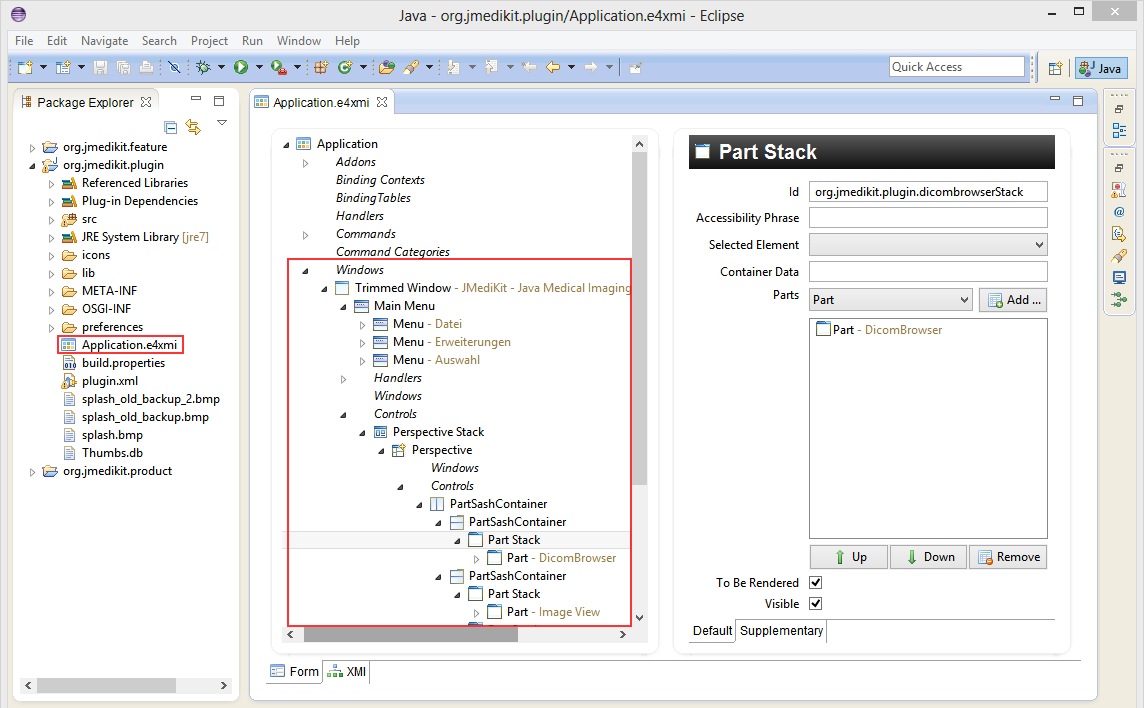
\includegraphics[angle=0,width=8cm]{./img/part_exmi.png}}
   \caption{Die Datei Application.e4xmi}
  \label{e4xmi}
  \vspace{0.5cm}
\end{figure}

Nach der Auswahl des \textit{PartStack}-Elements sind rechts dessen Eigenschaften inklusive einer Liste aller enthaltenen \textit{Parts} zu sehen(Abbildung \ref{partadd}). Über das Formularfeld \textit{Parts} kann mit einem Klick auf \textit{Add} ein neuer Kindknoten eingefügt werden. Im diesem Beispiel wird dem Stack ein neuer \textit{Part} untergeordnet.

\begin{figure}[H]
  \vspace{0.5cm}
  \centering
  \fbox{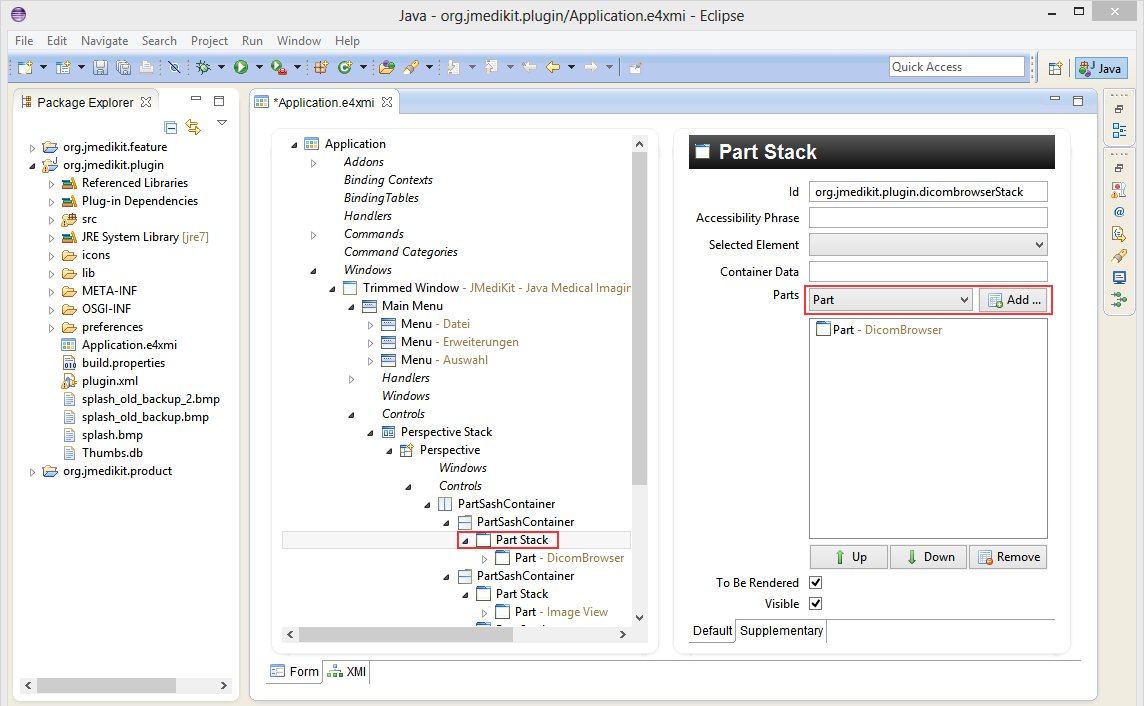
\includegraphics[angle=0,width=8cm]{./img/part_add.png}}
   \caption{Einfügen der Part-Struktur}
  \label{partadd}
  \vspace{0.5cm}
\end{figure}

Folgend öffnen sich rechts die Eigenschaften des neu angelegten Parts. Wichtige Einstellungen sind \textit{Id}, \textit{Label} und \textit{ClassURI}. Mit Hilfe der Id kann der Part im Quelltext referenziert werden und das Label ist der sichtbare Titel des \textit{Parts} in der Anwendung. Noch ist keine Klasse für das neue Strukturelement definiert worden. Dies kann mit einem Klick auf \textit{ClassURI} erledigt werden. Soll ein Icon neben dem Titel erscheinen, muss zuvor eine Bilddatei nach der Anleitung in Anhang \ref{importicon} importiert werden\footnote{Grundsätzlich ist es ausreichend die Bilddateien im \textit{icon}-Ordner zu speichern, aufgrund einer durchgehenden Konsistenz ist es allerdings besser das Bild komplett zu importieren}.

\begin{figure}[H]
  \vspace{0.5cm}
  \centering
  \fbox{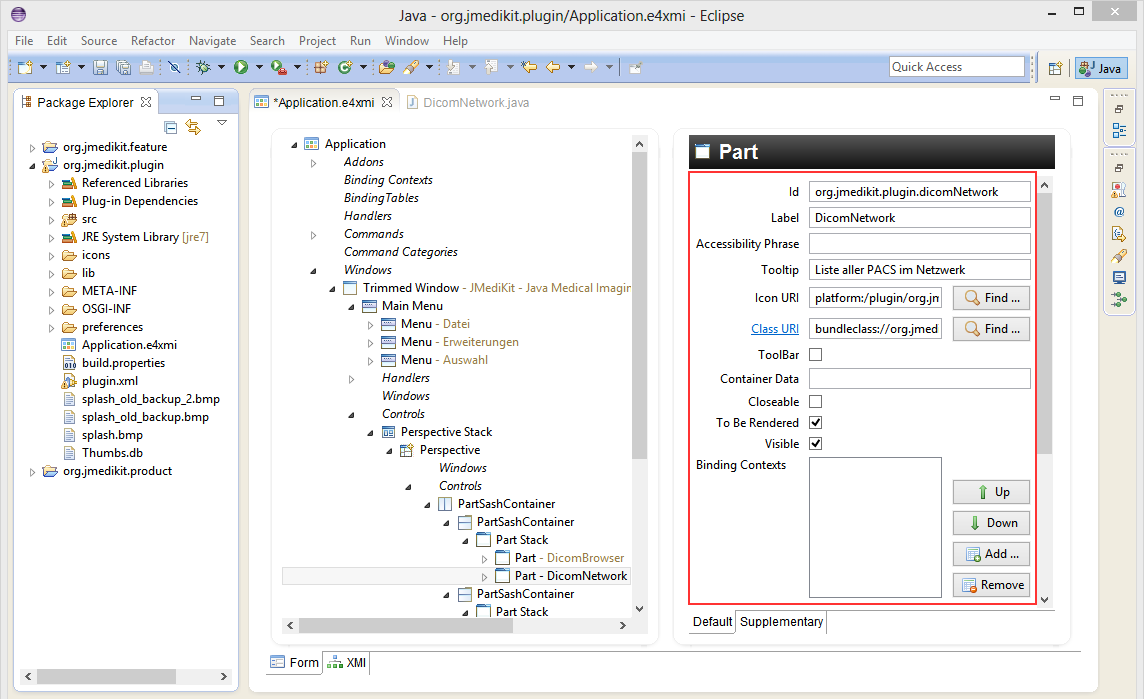
\includegraphics[angle=0,width=8cm]{./img/part_part.png}}
   \caption{Einfügen der Part-Struktur}
  \label{partpart}
  \vspace{0.5cm}
\end{figure}

Die zu erstellende Klasse repräsentiert neben der Benutzeroberfläche auch die Logik hinter dem \textit{Part}. Abbildung \ref{partclass} zeigt den Dialog zum Erstellen dieser Klasse. Alle \textit{Part}-Implementierungen befinden sich im Package \textit{org.jmedikit.plugin.gui}. Der Name ist frei wählbar. Neben Package und Klassenname kann aus vier vordefinierten Methoden gewählt werden.

\begin{figure}[H]
  \vspace{0.5cm}
  \centering
  \fbox{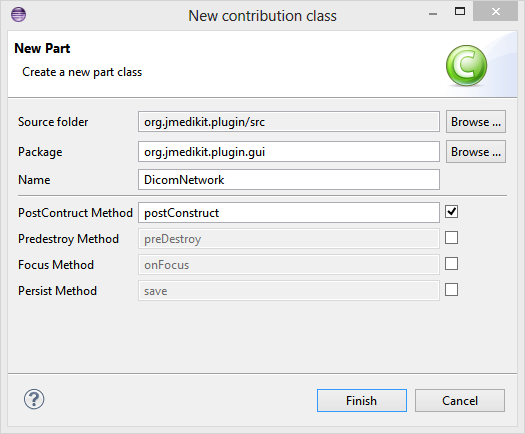
\includegraphics[angle=0,width=6cm]{./img/part_class.png}}
   \caption{Erstellen der Klasse}
  \label{partclass}
  \vspace{0.5cm}
\end{figure}

Listing \ref{partexample} zeigt eine Beispielimplementierung des \textit{Parts}. Die Annotation \textit{@PostConstruct} sorgt dafür, dass die Methode automatisch nach dem Instantiieren des Objekts ausgelöst wird. Diese enthält als Paramter ein \textit{Composite} und stellt den Einhängepunkt für die weitere Benutzeroberfläche dar.

\lstset{
language=Java,
caption={Erweiternder Eintrag einer Konstanten in der Klasse \textit{ImageProvider}},
label=partexample,
xleftmargin=1em,
xrightmargin=1em,
numbers=left,
backgroundcolor=\color{lgrey},
}  
\begin{figure}[htbp]
\begin{lstlisting}[frame=leftline]
//imports

public class DicomNetwork {

  @PostConstruct
  public void postConstruct(Composite parent) {
	
    //definiert das Layout des Elternelements
    //2 Spalten mit gleicher Breite
    GridLayout pGrid = new GridLayout(2, true);
    GridData parentData = new GridData(GridData.FILL_HORIZONTAL);
    
    parent.setLayout(pGrid);
    parent.setLayoutData(parentData);

    //GUI

    //Suchfeld
    Text search = new Text(parent, SWT.BORDER);
    
    //Suchbutton
    Button button = new Button(parent, SWT.NONE);
    button.setText("Suche PACS");	
  }	
}
\end{lstlisting}
\end{figure}

Abbildung \ref{partfinal} zeigt den neuen \textit{Part} in der linken Spalte der Anwendung. Damit wurde dem \textit{PartStack} in dem der \textit{DicomBrowser} enthalten ist das neue \textit{DicomNetwork} eingefügt.

\begin{figure}[H]
  \vspace{0.5cm}
  \centering
  \fbox{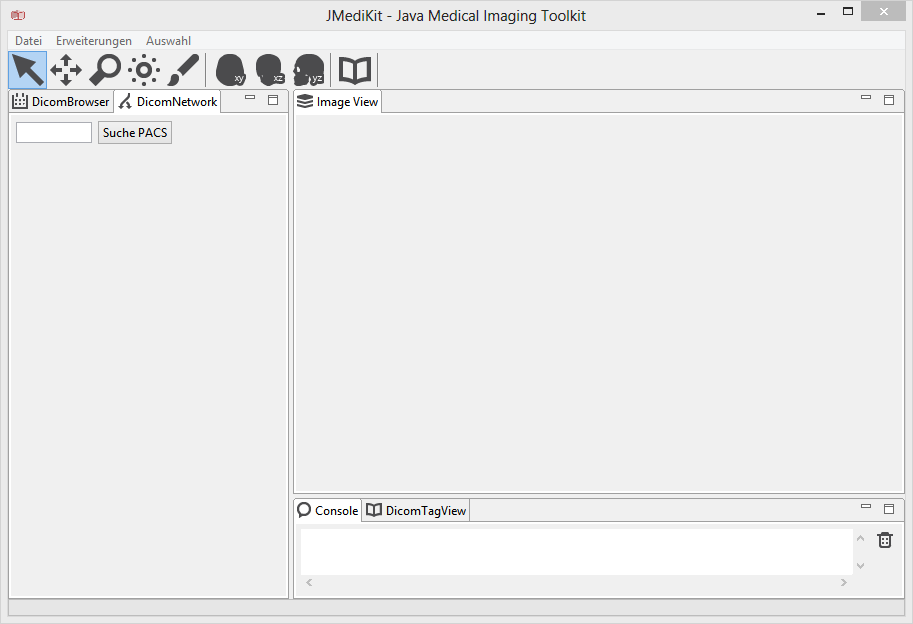
\includegraphics[angle=0,width=8cm]{./img/part_final.png}}
   \caption{Anzeige des Parts im PartStack}
  \label{partfinal}
  \vspace{0.5cm}
\end{figure}

\section{Erweiterung der Werkzeuge}
Im folgenden Abschnitt wird der Werkzeugleiste ein weiteres Tool hinzugefügt. Ähnlich dem \textit{PointTool} sollen Bildbereiche ausgewählt werden. Der Unterschied besteht darin, dass keine Punkte bestimmt werden, sondert ein rechteckiger Bildbereich als \textit{Region Of Interest}(ROI) markiert werden kann. Damit werden die Selektionswerkzeuge um das \textit{ROITool erweitert}.\\

\subsection{Hinzufügen eines Menüpunktes}

Das Menü selbst befindet sich im Applikationsbaum \textit{Window} unter dem Element \textit{TrimBars} $\rightarrow$ \textit{WindowTrim - Top} $\rightarrow$ \textit{ToolBar} und enthält \textit{HandledToolItems}-Strukturen des Application Models als Menüpunkte (Abbildung \ref{toolmenu}). Das bedeutet, dass zu jedem Eintrag ein \textit{Command} mit dem zugehörigen \textit{Handler} erstellt werden muss.

\begin{figure}[H]
  \vspace{0.5cm}
  \centering
  \fbox{\includegraphics[angle=0,width=8cm]{./img/tool_menu.png}}
   \caption{Die Werkzeugleiste im Application Model}
  \label{toolmenu}
  \vspace{0.5cm}
\end{figure}

Die \textit{Commands} sind im Strukturbaum direkt unter \textit{Application} zu finden. Wird das Element ausgewählt, erscheint auf der rechten Seite eine Liste bisher verfügbarer \textit{Commands}. Mit einem Klick auf \textit{Add} kann ein neuer hinzugefügt werden. In den nun angezeigten Einstellungen bekommt die \textit{Id} den Wert \textit{org.jmedikit.plugin.command.toolRoi} und als \textit{Name} wird \textit{toolRoi} eingetragen.\\
Die Implementierung der Befehle finden in den \textit{Handlern} statt. Diese sind im Baum unter \textit{Window} angesiedelt. Nach der Auswahl erscheint die Liste der erstellten \textit{Handler}. Wie schon bei den \textit{Commands} wird ein neuer \textit{Handler} hinzugefügt und \textit{Id} sowie \textit{Name} vergeben. Unter dem Punkt \textit{Command} wird der zuvor erstellte Befehl angegeben. Mit einem Klick auf \textit{ClassURI}, wie in Abbildung \ref{tool_handlerclass} dargestellt, kann die entsprechende Klasse erstellt werden. Üblicherweise liegen Handlerklassen im Package \textit{org.jmedikit.plugin.gui.handler} und haben den Namen \textit{ToolNameHandler}.

\begin{figure}[H]
  \vspace{0.5cm}
  \centering
  \fbox{\includegraphics[angle=0,width=6cm]{./img/tool_handlerclass.png}}
   \caption{Erstellung einer Klasse für die Handlerimplementierung}
  \label{tool_handlerclass}
  \vspace{0.5cm}
\end{figure}

Im nächsten Schritt erfolgt das Hinzufügen eines \textit{HandledToolItem} zu dem Element unter \textit{Window} $\rightarrow$ \textit{TrimBars} $\rightarrow$ \textit{WindowTrim - Top} $\rightarrow$ \textit{ToolBar}. Die Reihenfolge der Liste entspricht der Darstellung in der Anwendung. Unter den Einstellungen muss \textit{Id}, \textit{Label} und \textit{Command} mit Werten belegt werden. Als \textit{Type} muss die Option \textit{Radio} gewählt werden, da genau ein Werkzeug aktiv ausgewählt sein darf. Unter dem Punkt \textit{IconURI} wird bei Bedarf ein Bild angegeben. Abbildung \ref{tool_handleditem} zeigt die gesetzten Einstellungen.

\begin{figure}[H]
  \vspace{0.5cm}
  \centering
  \fbox{\includegraphics[angle=0,width=8cm]{./img/tool_handleditem.png}}
   \caption{Einstellungen des neuen Menüpunktes}
  \label{tool_handleditem}
  \vspace{0.5cm}
\end{figure}

Abbildung \ref{tool_menunew} zeigt die neue Werkzeugleiste mit dem \textit{ROITool} als erweiterten Eintrag.

\begin{figure}[H]
  \vspace{0.5cm}
  \centering
  \fbox{\includegraphics[angle=0,width=8cm]{./img/tool_menunew.png}}
   \caption{Anzeige der erweiterten Werkzeugleiste}
  \label{tool_menunew}
  \vspace{0.5cm}
\end{figure}

\subsection{Hinzufügen der Funktionalität}

Nach der Erweiterung der Werkzeugleiste kann die grundlegende Klasse des Werkzeugs erstellt werden. Wichtig ist die Generalisierung von \textit{ATool}, wie in Listing \ref{toolclass} zu sehen ist.

\lstset{
language=Java,
caption={Erweiterung des Basiswerkzeugs},
label=toolclass,
xleftmargin=1em,
xrightmargin=1em,
numbers=left,
backgroundcolor=\color{lgrey},
}  
\begin{figure}[htbp]
\begin{lstlisting}[frame=leftline]
public class RoiTool extends ATool{

  public RoiTool(DicomCanvas c) {
    super(c);
    System.out.println("Hello ROITool");
  }
  
  //weitere Implementierungen abstrakter Methoden
  //der Klasse ATool
}
\end{lstlisting}
\end{figure}

Wird der Menüpunkt in der Werkzeugleiste betätigt, werden Events ausgelöst. In der Klasse \textit{EventConstants} sind diese jeweils in Gruppen definiert. Die Wurzel einer Gruppe hat die in Listing \ref{groups} dargestellte Struktur. \textit{TOOL\_CHANGED} ist der Gruppenname der Events, die Werkzeuge betreffen. Der Zusatz \textit{/*} symbolisiert die Wurzel. Ein spezifisches Werkzeug hat die Form \textit{TOOL\_CHANGED/TOOLNAME}. Durch die Gruppenmechanik ist es möglich, dass eine spezielle Funktion auf alle Werkzeug-Events lauscht und abhängig vom Event die Aufgaben delegiert.

\lstset{
language=Java,
caption={Eventkonstanten der Klasse EventConstants},
label=groups,
xleftmargin=1em,
xrightmargin=1em,
numbers=left,
backgroundcolor=\color{lgrey},
}  
\begin{figure}[htbp]
\begin{lstlisting}[frame=leftline]
public final static String TOOL_CHANGED_ALL = "TOOL_CHANGED/*";
public final static String TOOL_CHANGED_ALL = "TOOL_CHANGED/POINT";
public final static String TOOL_CHANGED_ALL = "TOOL_CHANGED/ROI";
\end{lstlisting}
\end{figure}

Nachdem die Tool-Klasse und das Event kreiert wurden, kann das neue Werkzeug der Fabrik, die für die Erzeugung der Objekte zuständig ist, bekannt gemacht werden. Da das \textit{ROITool} zum Bereich der Selektion gehört, wird die Klasse \textit{SelectionToolFactory} angepasst. In Listing \ref{factory} werden die Modifikationen dargestellt. Innerhalb der Fabrik werden die zugehörigen Events in einer Konstante gespeichert. Die Methode \textit{produce} regelt die Objekterzeugung. Klickt der Anwender auf den Menüpunkt \textit{ROITool} wird das Event ausgelöst und der Werkzeugname an die Fabrik übergeben. Aufgrund des \textit{toolname} wird das richtige Werkzeug erstellt.

\lstset{
language=Java,
caption={Modifikation der SelectionToolFactory},
label=groups,
xleftmargin=1em,
xrightmargin=1em,
numbers=left,
backgroundcolor=\color{lgrey},
}  
\begin{figure}[htbp]
\begin{lstlisting}[frame=leftline]

public final static String ROI_TOOL = 
  EventConstants.TOOL_CHANGED_ROI;
//weitere Konstanten

@Override
protected ATool produce(String toolname, DicomCanvas c) {
  //Pruefung vorheriger Werkzeuge
  else if(toolname.equals(ROI_TOOL)){
    return new RoiTool(c);
  }
  //Pruefung folgender Werkzeuge
  //Werkzeug wurde nicht gefunden
  else throw new IllegalArgumentException("ERROR");
}
\end{lstlisting}
\end{figure}

Im aktuellen Zustand reagiert das Werkzeug und der neue Menüpunkt noch nicht auf die Eingaben des Benutzers. Es fehlt die Implementierung des \textit{Handlers} und die Kommunikation mit dem \textit{ImageView}. Listing \ref{roihandler} zeigt die Umsetzung der Klasse \textit{ToolRoiHandler}. Das Interface \textit{IEventBroker} regelt die Kommunikation unter den \textit{Parts}. Die Annotation \textit{@Execute} bedeutet, dass die Methode automatisch aufgerufen wird, sobald der Menüpunkt betätigt wird. Sowohl \textit{@Inject} als auch \textit{@Execute} sind Teile des \textit{Dependency Injection Frameworks} von Eclipse. Ein umfassender Artikel ist unter \cite{vogel:di} zu finden.\\
In der Methode \textit{execute} wird dem Werkzeug entsprechend die Fabrik instantiiert. Die Variable \textit{tool} enthält das auszulösende Event. Mit Hilfe des \textit{eventBroker} wird die Benutzereingabe an die lauschenden Methoden der Applikation geleitet. Die Methode \textit{post} erwartet die Event-Konstante und ein ToolEvent, welches die erzeugte Fabrik und den Werkzeugtyp als Parameter erhält.

\lstset{
language=Java,
caption={Implementierung des ToolRoiHandler},
label=roihandler,
xleftmargin=1em,
xrightmargin=1em,
numbers=left,
backgroundcolor=\color{lgrey},
}  
\begin{figure}[htbp]
\begin{lstlisting}[frame=leftline]
@Inject
IEventBroker eventBroker;

@Execute
public void execute() {

  AToolFactory factory = new SelectionToolFactory();
  String tool = EventConstants.TOOL_CHANGED_ROI;

  eventBroker.post(EventConstants.TOOL_CHANGED_ROI, new SelectionToolEvent(factory, tool));
}
\end{lstlisting}
\end{figure}

Klickt der Benutzer auf den Menüpunkt nachdem der \textit{Handler} implementiert wurde, erfolgt die Ausgabe \glqq Hello ROITool\grqq\ auf der Standardausgabe. Das bedeutet, das Werkzeug wurde korrekt erzeugt und kann verwendet werden. Der nächste Schritt ist die Implementierung der Logik.

\subsection{Hinzufügen der Werkzeuglogik}

Ziel des \textit{ROITools} ist es, beliebige rechteckige Flächen innerhalb des Bildes zu markieren, um diese später in Plug-ins benutzen zu können. So können Algorithmen auf ausgewählten Bildbereichen angewendet werden. Folgende Events werden von dem neuen Werkzeug behandelt:

\begin{itemize}
\item \textbf{MouseMove} \\
Bei jeder Mausbewegung wird geprüft, ob eine Maustaste gedrück wird. Ist dies der Fall, wird die Startposition und die Aktuelle solange in Datenelementen der Klasse gespeichert, bis die Taste gelöst wird.
\item \textbf{MouseDown} \\
Wird die Maustaste betätigt, werden die Koordinaten auf $0$ zurückgesetzt, damit eine neue Berechnung beginnen kann. Ohne Zurücksetzung wird die zuletzt markierte ROI nochmal auf die Zeichenfläche gemalt und bleibt bis zur ersten Mausbewegung sichtbar.
\item \textbf{MouseUp} \\
 Befindet sich nach dem Loslassen der Maustaste der Start- und Endpunkt des Cursors innerhalb des Bildes, wird eine \textit{Region Of Interest} berechnet. Dazu werden zuerst die Bildkoordinaten der beiden Punkte ermittelt. Darauf folgt eine Normalisierung der Koordinaten und ein Eintrag der im Anschluss erzeugten ROI im Bild.
\item \textbf{PostCalculation} \\
Nach der Werteberechnung wird das Rechteck der potentiellen ROI auf der Zeichenfläche dargestellt.
\end{itemize}


Ist die Logik implementiert, kann das Werkzeug in vollem Umfang eingesetzt werden. Das Erstellen von Transformationstypen erfolgt analog zu den Selektionswerkzeugen. Eine erweiterte Implementierung des \textit{ROITools} könnte zum Beispiel eine dynamische Größenanpassung der Fläche mit dem Mausrad realisieren.
%Nachdem dem Erstellen des Menüeintrags kann die Fabrik, die für die Erzeugung der Werkzeuge verantwortlich %ist, erweitert werden.

\chapter{Diskussion}
\addthumb{Diskussion}{\huge{\textbf{\thechapter.}}}{white}{haw_rot} 

Für eine erfolgreiche Umsetzung der Arbeit stehen die Anforderungen an die Modularität und Erweiterbarkeit der zu entwickelnden Software und die Methoden zur Bildanzeige und Manipulation im Fokus. 

\section*{Modularität}

Mit dem Einsatz der \glqq Eclipse Rich Client Platform\grqq\ und dem zugehörigen OSGi-Framework \glqq Equinox\grqq\ wird eine modulare Anwendungsstruktur geschaffen. Durch das Hinzufügen von neuen Strukturelementen des Application Models und deren Implementierung kann jMediKit um neue Module erweitert werden. Dadurch wird die Tiefe der Anwendung mit den zur Verfügung stehenden Grundfunktionen erweitert. So ist es zum Beispiel möglich, die Anwendung um einen Bereich zu erweitern, der aus den Voxeldaten dreidimensionale Darstellungen berechnet.\\
Um neue Module zu entwickeln, ist neben der Kenntnis der Struktur von jMediKit auch eine Einarbeitung in die Architektur der Eclipse-Plattform notwendig. Die Werkzeuge sind zum Beispiel fest mit der jMediKit-Architektur durch das Fabrikmuster verankert. Für eine Erweiterung benötigt ein Entwickler das Wissen zu Werkzeugleisten der Eclipse-Plattform und zur Werkzeugentwicklung von jMediKit. Zusätzlich können neue Funktionen ausschließlich nach einem erneuten Buildprozess der Anwendung hinzugefügt werden. Dadurch ist keine dynamische Modulerweiterung des aktuellen Systems möglich.

\pagebreak

\section*{Erweiterbarkeit}
Das Architekturmuster Plug-in stellt diesen dynamischen Aspekt der Anwendungserweiterung zur Verfügung. Das bedeutet, Klassen können auch nach der Kompilierung zu dem System hinzugefügt werden. Dadurch wird eine Erweiterung möglich, ohne genaue Kenntnis des Systems und seine interne Funktionsweise besitzen zu müssen. Trotz des dynamischen Charakters sind die vom Anwender entwickelten Erweiterungen auf die Aspekte der Bildverarbeitung beschränkt und können keine Beiträge zur Anwendungsstruktur leisten.

\section*{Bildanzeige und Manipulation}
Mit der Verwendung der externen Bibliothek \glqq dcm4che\grqq\ als Werkzeug zur Verarbeitung der DICOM-Daten, können medizinsche Bilddaten entsprechend der Anforderungen angezeigt und manipuliert werden.Da Algorithmen sowohl in der initialen Ebenendarstellung, als auch in den rekonstruierten Darstellungen angewendet werden sollen, wird der gesamte Datensatz beim Einlesen in den Speicher geladen. Dadurch hat jMediKit einen hohen Speicherbedarf. So benötigt allein die Anzeige von vier Datensätzen mit 512 Schichten und einer Auflösung von 512 $\times$ 512 Pixel und einer Tiefe von 16-Bit ca. 1 Gigabyte Speicherplatz rein an Daten der Pixelwerte.

\begin{equation}
(312^3 \cdot 16)\cdot 4  = 8589934592 bit = 1 GB
\end{equation}

In der initialen Ebenendarstellung könnten Bildschichten problemlos bei Bedarf nachgeladen werden. Ein dreidimensionaler Algorithmus ist zur Berechnung allerdings abhängig von den restlichen Schichten. Auch Ebenenrekonstruktionen benötigen den gesamten Datensatz. Ein dynamisches Nachladen bei der Algorithmenanwendung und Rekonstruktion verlängert die Ausführungszeit des Programms und es musste die Wahl zwischen einem hohen Speicherbedarf und schneller Bedienung oder geringem Speicherbedarf bei verzögerter Bedienung getroffen werden.\\
So könnten zukünftige Weiterentwicklungen einen Kompromiss zwischen Speicher und Ausführungszeit finden, um eine verbesserte Lösung zur Verfügung zu stellen. Caching-Algorithmen wären in der Lage den Ladevorgang und die Speicherung effizient zu verwalten.



\chapter{Fazit}
\addthumb{Fazit}{\huge{\textbf{\thechapter.}}}{white}{haw_rot} 
Die qualitativen Anforderungen der Modularität und Erweiterbarkeit an Architektur und Programmeigenschaften werden mit Hilfe einer überaus flexiblen Anwendungsstruktur umgesetzt, die eine Erweiterung an den entscheidenden Stellen zulässt. So ist sowohl eine statische Erweiterung durch Module und Werkzeuge, als auch eine dynamische durch Plug-ins in zwei- und dreidimensionalem Raum möglich.\\
Die funktionalen Anforderungen an die Software decken im Besonderen die Anzeige und Manipulation der Bilder sowie die dynamische Parameterübergabe ab. Die Bildanzeige kann zur Navigation und Orientierung im 3D-Datensatz verwendet werden und bietet typische Operationen wie die Translation und die Skalierung. Mit Hilfe der Selektionswerkzeuge können zusätzlich für den Anwender wichtige Bereiche markiert und in Plug-ins interpretiert werden.\\
JMediKit setzt die Anforderungen an die Software und deren Architektur um und liefert eine solide Grundlage für zukünftige Erweiterungen. Denkbar wäre eine Anbindung an das Picture Archiving and Commnication System des Labors, um medizinische Bilder direkt aus dem Netzwerk beziehen zu können. Zusätzlich könnte ein 3D-Renderer integriert werden, der eine dreidimensionale Darstellung des Voxelraums bietet.
Das Java Medical Imaging Toolkit bietet dazu sowohl das Potential, als auch die Schnittstellen und stellt damit eine modulare und erweiterbare Anwendung zur medizinischen Bildverarbeitung dar.


\pagebreak

\bookmarksetup{startatroot}

\setcounter{page}{1}
\renewcommand{\thepage}{\Roman{page}}

%Literatur
%\addcontentsline{toc}{section}{Literaturverzeichnis}
%\setcounter{lofdepth}{2}
\stopthumb
%\bibliographystyle{alpha}
\bibliographystyle{alphadin}  
\bibliography{literature}

%\addcontentsline{toc}{section}{Abbildungsverzeichnis}
\listoffigures
\listoftables

\lstlistoflistings

\part{Anhang}

\appendix
\chapter{Darstellung der DICOM-Elemente im Speicher} \label{appendix:speicher}
\section{Explizite VR mit [ OB \textpipe\ OW \textpipe\ OF \textpipe\ SQ \textpipe\ UT \textpipe\ UN ]}

Bei expliziter VR-Struktur besteht das Element aus vier konsekutiven Feldern. Ist die VR vom Typ OB, OW, OF, SQ, UT oder UN wird das Datenelement wie in Tabelle \ref{table:appendix_explizit} im Speicher abgelegt. Die reservierten 2 Byte im VR-Teil sind für zukünftige Weiterentwicklungen des DICOM-Standards.\cite[7.1.2]{dicom:structure}

\begin{sidewaystable}
    \begin{tabularx}{\textwidth}{|X|X|p{5cm}|X|X|p{8cm}|}
    \toprule \hline
   \multicolumn{2}{|l|}{\textbf{Tag}} 	&	\multicolumn{2}{l|}{\textbf{VR}} 		&		\textbf{Value Length}   	& 	\textbf{Value} \\ \hline
    Group \# 16-bit unsigned integer & Element \# 16-bit unsigned integer  &  VR 2-byte character String [OB | OW | OF | SQ | UT | UN ] & Reservierter
    Bereich & 32-bit unsigned integer  &  Gerade Anzahl an Byte. Enthält den Wert des Datenelements. Kodierung abhängig von VT-Typ und Transfersyntax. Wenn die Länge nicht definiert ist wird diese auf \glqq Sequence Delimitation\grqq\ limitiert. \\ \hline
	
	2 Byte & 2 Byte & 2 Byte & 2 Byte & 4 Byte & Anzahl an Byte entsprechend der \glqq Value Length\grqq\, wenn von explizieter Länge \\ \hline
	
	\bottomrule
    \end{tabularx}
    \caption {Darstellung des Datenelements im Speicher wenn VR vom Typ OB, OW, OF, SQ, UT oder UN}
    \label{table:appendix_explizit}
\end{sidewaystable}

\section{Explizite VR}

Diese Darstellung wird gewählt wenn VR \textit{nicht} vom Typ OB, OW, OF, SQ, UT oder UN ist. Der Unterschied besteht im Feld \glqq Value Length\grqq\. Bei der Form von Tabelle \ref{table:appendix_explizit} ist dieses Feld 32 Bit lange. Hier beträgt es lediglich 16 Bit \cite[7.1.2]{dicom:structure}. Der Grund liegt am erhöhten Speicherbedarf von \ref{table:appendix_explizit}, da die Länge des Wertes eine undefinierte Länge haben kann.

\begin{sidewaystable}
	\begin{tabularx}{\textwidth}{|X|X|X|X|p{12cm}|}
	\toprule \hline
	\multicolumn{2}{|l|}{\textbf{Tag}} & \textbf{VR} 2 & \textbf{Value Length} & \textbf{Value} 4 \\ \hline
	Group \# 16-bit unsigned integer & Element \# 16-bit unsigned integer & VR 2-byte character String 2 & 16-bit unsigned integer & Gerade Anzahl an Byte. Enthält den Wert des Datenelements. Kodierung abhängig von VT-Typ und Transfersyntax. \\ \hline
	2 Byte & 2 Byte & 2 Byte & 2 Byte & \glqq Value Length\grqq\ Byte \\ \hline
	\bottomrule
	\end{tabularx}
    \caption {Darstellung des Datenelements für alle anderen VR-Typen}
    \label{table:appendix_explizit_else}
\end{sidewaystable}

\section{Implizite VR}

Bei einer impliziten VR Darstellung besteht das Datenelement aus den drei konsekutive Feldern Tag, Value Length und dem Wert selbst \cite[7.1.3]{dicom:structure}.

\begin{sidewaystable}
	\begin{tabularx}{\textwidth}{|X|X|X|p{12cm}|}
	\toprule \hline
	\multicolumn{2}{|l|}{\textbf{Tag}} & \textbf{Value Length} 2 & \textbf{Value} \\ \hline
	Group \# 16-bit unsigned integer & Element \# 16-bit unsigned integer & 32-bit unsigned integer & Gerade Anzahl an Byte. Enthält den Wert des Datenelements. Kodierung abhängig von VT-Typ spezifiziert in \cite{dicom:dd} und Transfersyntax. Wenn die Länge nicht definiert ist wird diese auf \glqq Sequence Delimitation\grqq\ limitiert. \\ \hline
	2 Byte & 2 Byte & 2 Byte & \glqq Value Length\grqq\ Byte oder undefinierte Länge \\ \hline
	
	\bottomrule
	
	\end{tabularx}
    \caption {Darstellung des Datenelements für implizite VR.}
    \label{table:appendix_implizit}
\end{sidewaystable}



\end{document}